% !TeX program = xelatex
\documentclass[11pt,a4paper]{article}

% -------------------------------------------------
% Packages
% -------------------------------------------------
\usepackage{kotex}
\usepackage{fontspec}
\usepackage{amsmath,amssymb,bm,mathtools}
\usepackage[left=24mm,right=24mm,top=23mm,bottom=25mm]{geometry}
\usepackage{booktabs,array}
\usepackage{enumitem}
\usepackage{setspace}
\usepackage{xcolor}
\usepackage{colortbl}
\usepackage{tikz}
\usepackage{pifont}
\usetikzlibrary{positioning,arrows.meta,calc,fit,decorations.pathreplacing}
\usepackage[most]{tcolorbox}
\usepackage{listings}
\usepackage{hyperref}
\usepackage{fancyhdr}

\setstretch{1.14}
\setlength{\parindent}{0pt}
\setlength{\parskip}{0.55em}

% -------------------------------------------------
% Colors and boxes
% -------------------------------------------------
\definecolor{deepblue}{RGB}{34,71,120}
\definecolor{softblue}{RGB}{239,246,253}
\definecolor{softgray}{RGB}{246,247,249}
\definecolor{softgreen}{RGB}{239,249,242}
\definecolor{softyellow}{RGB}{255,249,229}
\definecolor{codegray}{RGB}{248,248,248}

\newtcolorbox{keybox}[1][]{
  colback=softblue,
  colframe=deepblue,
  boxrule=0.7pt,
  arc=2mm,
  title=#1,
  fonttitle=\bfseries
}

\newtcolorbox{thinkbox}[1][]{
  colback=softyellow,
  colframe=orange!70!black,
  boxrule=0.6pt,
  arc=2mm,
  title=#1,
  fonttitle=\bfseries
}

\newtcolorbox{remarkbox}[1][]{
  colback=softgray,
  colframe=black!45,
  boxrule=0.5pt,
  arc=2mm,
  title=#1,
  fonttitle=\bfseries
}

\newtcolorbox{mlbox}[1][]{
  colback=softgreen,
  colframe=green!45!black,
  boxrule=0.6pt,
  arc=2mm,
  title=#1,
  fonttitle=\bfseries
}

% -------------------------------------------------
% Code style
% -------------------------------------------------
\lstdefinestyle{pythonstyle}{
  language=Python,
  backgroundcolor=\color{codegray},
  basicstyle=\ttfamily\small,
  keywordstyle=\bfseries,
  commentstyle=\itshape\color{black!60},
  stringstyle=\color{black!75},
  numbers=left,
  numberstyle=\tiny\color{black!55},
  numbersep=8pt,
  frame=single,
  rulecolor=\color{black!25},
  breaklines=true,
  showstringspaces=false,
  tabsize=4,
  columns=fullflexible,
  keepspaces=true
}
\lstset{style=pythonstyle}

% -------------------------------------------------
% Math commands
% -------------------------------------------------
\newcommand{\R}{\mathbb{R}}
\newcommand{\grad}{\nabla}
\newcommand{\vect}[1]{\bm{#1}}
\newcommand{\T}{^{\mathsf T}}
\newcommand{\loss}{\mathcal{L}}
\newcommand{\sigmoid}{\sigma}
\newcommand{\pd}[2]{\frac{\partial #1}{\partial #2}}
\newcommand{\softmax}{\operatorname{softmax}}

% -------------------------------------------------
% Header / footer
% -------------------------------------------------
\pagestyle{fancy}
\fancyhf{}
\lhead{Introduction to Deep Learning and Practice}
\rhead{Techniques for Training}
\cfoot{\thepage}
\renewcommand{\headrulewidth}{0.4pt}
\setlength{\headheight}{14pt}

\hypersetup{
  colorlinks=true,
  linkcolor=deepblue,
  urlcolor=deepblue
}

% =================================================
\begin{document}
% =================================================

\begin{center}
{\LARGE\bfseries 학습 관련 기술}\\[0.35em]
{\large 매개변수 갱신 $\cdot$ 가중치의 초깃값 $\cdot$ 배치 정규화 $\cdot$ 바른 학습을 위해 $\cdot$ 하이퍼파라미터}\\[0.35em]
{\normalsize SGD $\rightarrow$ Momentum $\rightarrow$ AdaGrad $\rightarrow$ RMSProp $\rightarrow$ Adam $\rightarrow$ Xavier $\cdot$ He 초기화 $\rightarrow$ Batch Norm $\rightarrow$ Weight Decay $\cdot$ AdamW $\cdot$ Dropout}\\[0.8em]
\end{center}

\vspace{0.4em}

\begin{keybox}[이번 주의 핵심 질문]
지난주에는 역전파로 손실의 gradient $\pd{L}{W}$를 계산하고,
\[
W\leftarrow W-\alpha\pd{L}{W}
\]
로 매개변수를 갱신하여 MNIST를 학습시켰다.
그런데 이 갱신 규칙이 최선일까?
gradient가 가리키는 방향이 늘 최솟값을 향하는 것은 아니고,
학습률 $\alpha$ 하나로 모든 매개변수를 같은 비율로 움직이는 것도 비효율적일 수 있다.
\textbf{같은 gradient 정보를 쓰되, 더 빠르고 안정적으로 최솟값을 찾아가는 방법}은 무엇일까?
\end{keybox}

\subsection*{학습목표}

이 주차가 끝나면 다음을 설명하고 직접 계산할 수 있어야 한다.

\begin{enumerate}[label=\arabic*.]
\item 신경망 학습을 최적화 문제로 보고, 매개변수 갱신 규칙의 역할을 설명한다.
\item 확률적 경사하강법(SGD)이 방향에 따라 곡률이 다른 함수에서 지그재그로 움직이는 이유를 설명한다.
\item 모멘텀이 과거 gradient를 누적하여 진동을 줄이고 가속하는 원리를 설명한다.
\item AdaGrad와 RMSProp이 매개변수마다 학습률을 다르게 조절하는 원리를 설명한다.
\item Adam의 갱신 규칙과 편향 보정(bias correction)을 설명한다.
\item 각 최적화 기법을 \texttt{update(params, grads)} 형태의 코드로 구현한다.
\item 초기 가중치가 은닉층의 활성화값 분포와 학습에 주는 영향(기울기 소실, 표현력 제한)을 설명한다.
\item Xavier 초깃값과 He 초깃값을 분산이 유지되는 조건으로부터 유도한다.
\item 배치 정규화의 순전파 식과 계산 그래프를 이해하고, 역전파를 유도하여 구현한다.
\item 학습할 때와 추론할 때 배치 정규화가 다르게 동작하는 이유를 설명한다.
\item 오버피팅을 훈련 정확도와 시험(검증) 정확도의 차이로 확인하고, 그 원인을 설명한다.
\item 가중치 감소(L2 규제, AdamW)와 드롭아웃의 원리를 설명하고 구현한다.
\item 훈련 / 검증 / 시험 데이터의 역할을 구분하고, 하이퍼파라미터를 시험 데이터로 고르면 안 되는 이유를 설명한다.
\item 로그 눈금의 무작위 탐색으로 하이퍼파라미터를 찾는다.
\end{enumerate}

% =================================================
\section{매개변수 갱신: 최적화 문제}
% =================================================

\subsection{신경망 학습은 최적화 문제이다}

신경망의 학습은 손실함수 $L(W)$를 가장 작게 만드는 매개변수 $W$를 찾는 문제,
즉 \textbf{최적화(optimization)} 문제이다.
매개변수의 개수는 MNIST의 작은 network만 해도 수만 개이고, 손실함수의 모양은 매우 복잡하여
최솟값을 식으로 한 번에 구할 수 없다.
그래서 지금까지 우리는 gradient를 단서로 하여 조금씩 매개변수를 고쳐 나가는 방법을 썼다.
이번 주에는 이 \textbf{갱신 규칙}을 개선하는 방법들을 살펴본다.

이 절 전체에서 다음 기호를 사용한다.
\begin{center}
\begin{tabular}{@{}ll@{}}
\toprule
기호 & 의미 \\
\midrule
$W$ & 갱신할 매개변수 (행렬이어도 된다) \\
$g_k=\pd{L}{W}\big|_{W=W_k}$ & $k$번째 단계의 gradient ($W$와 같은 shape) \\
$\alpha$ & 학습률 (learning rate) \\
$\odot$, $\sqrt{\cdot}$, $\dfrac{\cdot}{\cdot}$ & 성분별 곱, 성분별 제곱근, 성분별 나눗셈 \\
\bottomrule
\end{tabular}
\end{center}

\subsection{예제 함수: $f(x,y)=\frac{1}{20}x^2+y^2$}\label{sec:example}

여러 기법을 눈으로 비교하기 위해, 매개변수가 두 개뿐인 다음 함수의 최솟값을 찾는 문제를 생각하자.
\[
\boxed{
f(x,y)=\frac{1}{20}x^2+y^2,
\qquad
\nabla f(x,y)=\left(\frac{x}{10},\ 2y\right)
}
\]
최솟값은 $(0,0)$에서 $0$이다. 시작점은 모든 기법에서 $(x_0,y_0)=(-7,\ 2)$로 같게 둔다.

\IfFileExists{figures/opt_function.png}{%
\begin{center}
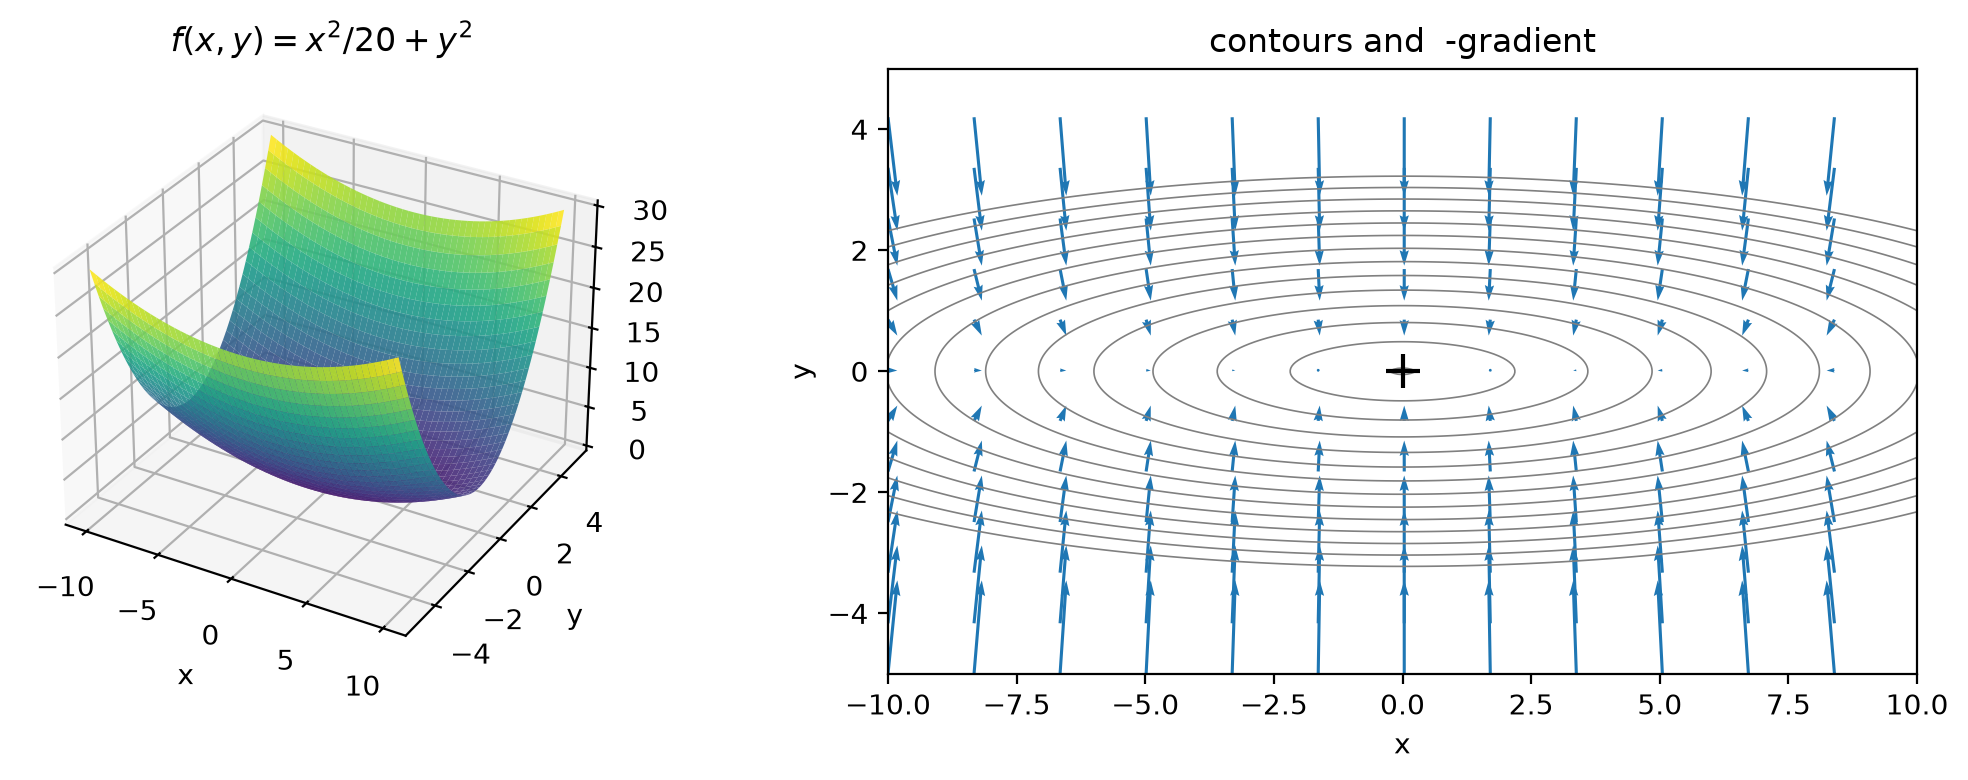
\includegraphics[width=\textwidth]{figures/opt_function.png}

\small $f(x,y)=x^2/20+y^2$의 그래프(왼쪽)와 등고선 및 $-\nabla f$의 방향(오른쪽)
\end{center}
}{%
\begin{center}
\fbox{\parbox{0.8\textwidth}{\centering\small
[그림 자리] \texttt{figures/opt\_function.png}\\
\texttt{optimizers\_2d.py}를 실행하면 생성된다.}}
\end{center}
}

이 함수는 $x$ 방향으로 아주 완만하고 $y$ 방향으로 가파른 \textbf{길고 좁은 골짜기} 모양이다.
두 방향의 곡률(이계도함수)은
\[
\frac{\partial^2 f}{\partial x^2}=\frac{1}{10},
\qquad
\frac{\partial^2 f}{\partial y^2}=2
\]
로 $20$배나 차이가 난다.
그래서 오른쪽 그림처럼 대부분의 점에서 $-\nabla f$는 최솟값 $(0,0)$이 아니라 거의 $y$축 방향(골짜기의 벽 쪽)을 가리킨다.
실제 딥러닝의 손실함수에서도 이처럼 방향마다 곡률이 크게 다른 경우가 흔하다.

이 예제에서 각 기법은 모두 같은 일을 반복한다.
현재 위치의 gradient $g_k=\nabla f(x_k,y_k)$를 계산하고, 갱신 규칙에 따라 다음 위치 $(x_{k+1},y_{k+1})$로 이동한다.
\textbf{달라지는 것은 오직 갱신 규칙뿐}이다.

\subsection{코드의 구조}

모든 최적화 기법을 같은 모양의 클래스로 만든다.
매개변수와 gradient를 같은 key를 가진 dictionary로 받아, \texttt{update} 메서드가 매개변수를 \textbf{제자리에서} 고친다.

\begin{lstlisting}
def f(x, y):
    return x ** 2 / 20.0 + y ** 2

def grad_f(x, y):
    return x / 10.0, 2.0 * y

def minimize(optimizer, start=(-7.0, 2.0), steps=30):
    """Run `steps` updates from `start`; return the path as an array of shape (steps+1, 2)."""
    params = {"x": np.array(start[0]), "y": np.array(start[1])}
    path = [(float(params["x"]), float(params["y"]))]
    for _ in range(steps):
        gx, gy = grad_f(params["x"], params["y"])
        grads = {"x": gx, "y": gy}
        optimizer.update(params, grads)
        path.append((float(params["x"]), float(params["y"])))
    return np.array(path)
\end{lstlisting}

\texttt{params}, \texttt{grads}는 지난주 \texttt{mnist\_lab.py}의 \texttt{network.params}, \texttt{grads}와 같은 형태이다.
따라서 이번 주에 만드는 optimizer는 MNIST 학습 루프의
\begin{lstlisting}
for key in network.params:
    network.params[key] -= learning_rate * grads[key]
\end{lstlisting}
부분을 \texttt{optimizer.update(network.params, grads)} 한 줄로 바꾸어 그대로 쓸 수 있다.

\paragraph{코드를 모듈로 나누기.}
optimizer 클래스는 2변수 예제에서도, MNIST 학습에서도 똑같이 쓰인다.
그래서 같은 코드를 파일마다 복사하지 않고, 공통 부분을 \textbf{모듈}(별도의 \texttt{.py} 파일)로 저장해 두고
필요한 곳에서 \texttt{import}하여 쓴다.
이번 주 코드는 모두 \texttt{code} 폴더에 있으며 다음과 같이 구성되어 있다.
어느 위치에서 실행하든 그림은 강의 노트 옆의 \texttt{figures} 폴더에 저장된다.

\begin{center}
\begin{tabular}{@{}lp{0.55\textwidth}@{}}
\toprule
파일 & 내용 \\
\midrule
\texttt{optimizers.py} & SGD, Momentum, AdaGrad, RMSProp, Adam 클래스 \\
\texttt{layers.py} & Affine, ReLU, Sigmoid, softmax 손실 계층, \texttt{MultiLayerNet} (지난주 코드) \\
\texttt{mnist\_data.py} & MNIST 불러오기, 정규화, one-hot, 훈련/검증 분할 \\
\midrule
\texttt{optimizers\_2d.py} & 2변수 예제 실험 (\texttt{optimizers.py} 사용) \\
\texttt{mnist\_optimizer\_compare.py} & MNIST 비교 실험 (\ref{sec:mnistopt}절, 세 모듈 모두 사용) \\
\bottomrule
\end{tabular}
\end{center}

예를 들어 2변수 예제 코드의 첫머리는 다음과 같다.
\begin{lstlisting}
import os
import numpy as np
import matplotlib.pyplot as plt

from optimizers import SGD, Momentum, AdaGrad, RMSProp, Adam   # optimizers.py
\end{lstlisting}
이후 각 기법을 설명할 때 보이는 클래스 코드는 모두 \texttt{optimizers.py}에 들어 있다.

% -------------------------------------------------
\subsection{확률적 경사하강법 (SGD)}\label{sec:sgd}
% -------------------------------------------------

\paragraph{갱신 규칙.}
지금까지 사용한 방법이다.
\[
\boxed{
W_{k+1}=W_k-\alpha\,g_k
}
\]
``\textbf{확률적}(stochastic)''이라는 이름은 $g_k$를 전체 데이터가 아니라
\textbf{무작위로 고른 미니배치}의 평균 손실로 계산하기 때문에 붙었다 (지난주 미니배치 학습).
예제 함수에는 데이터가 없으므로 정확한 gradient를 쓰지만, 갱신 규칙은 같다.

\begin{lstlisting}
class SGD:
    """W <- W - lr * dL/dW"""
    def __init__(self, lr=0.01):
        self.lr = lr

    def update(self, params, grads):
        for key in params:
            params[key] -= self.lr * grads[key]
\end{lstlisting}

\paragraph{예제에서의 움직임.}
$\nabla f=(x/10,\ 2y)$이므로 SGD의 갱신은 좌표마다 따로 쓸 수 있다.
\[
x_{k+1}=x_k-\alpha\frac{x_k}{10}=\Bigl(1-\frac{\alpha}{10}\Bigr)x_k,
\qquad
y_{k+1}=y_k-\alpha\cdot2y_k=(1-2\alpha)\,y_k
\]
즉 매 단계 $x$는 $\bigl(1-\frac{\alpha}{10}\bigr)$배, $y$는 $(1-2\alpha)$배가 된다.
(``Gradient Descent와 Newton's method'' 시간에 본 수렴 조건 $|1-\alpha f''|<1$이 방향마다 따로 적용되는 것이다.)

\begin{itemize}[leftmargin=1.8em]
\item $y$ 방향이 발산하지 않으려면 $|1-2\alpha|<1$, 즉 $\alpha<1$이어야 한다.
\item 그런데 $\alpha<1$이면 $x$ 방향의 비율은 $1-\frac{\alpha}{10}>0.9$로, $x$는 한 단계에 $10\%$도 줄지 않는다.
\end{itemize}
곡률이 큰 방향($y$) 때문에 학습률을 키울 수 없고,
그 작은 학습률로는 곡률이 작은 방향($x$)이 아주 느리게 수렴하는 것이다.

\IfFileExists{figures/opt_sgd_lr.png}{%
\begin{center}
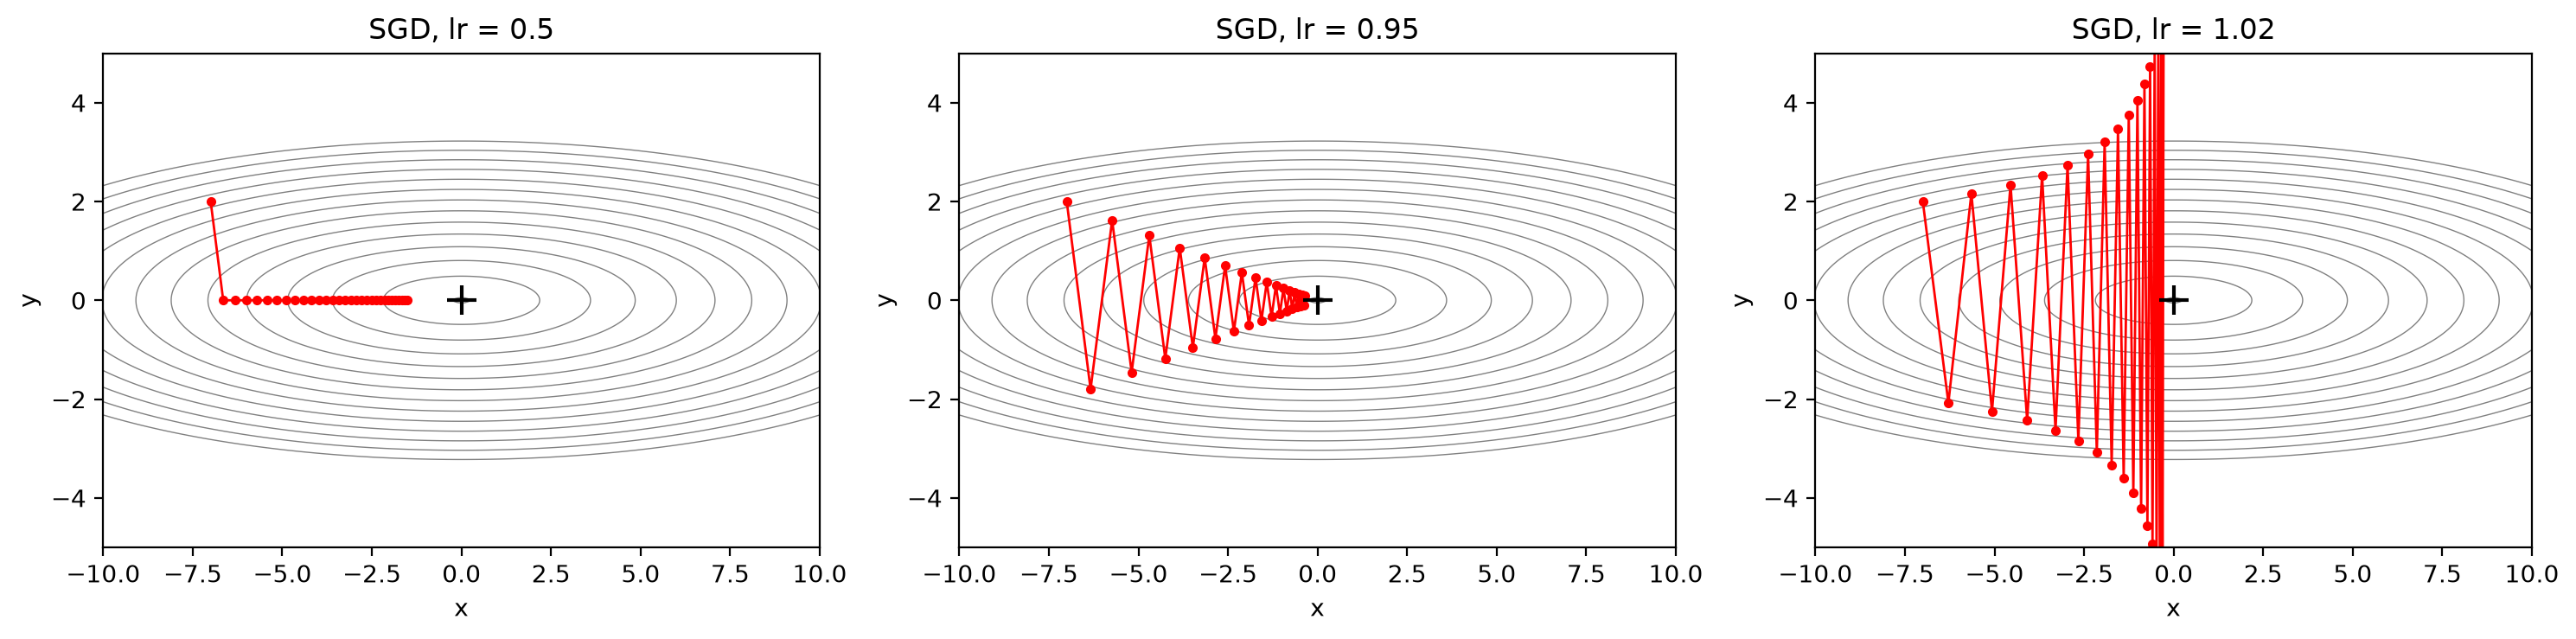
\includegraphics[width=\textwidth]{figures/opt_sgd_lr.png}

\small 학습률에 따른 SGD의 경로 (시작점 $(-7,2)$, $30$단계)
\end{center}
}{%
\begin{center}
\fbox{\parbox{0.8\textwidth}{\centering\small
[그림 자리] \texttt{figures/opt\_sgd\_lr.png}\\
\texttt{optimizers\_2d.py}를 실행하면 생성된다.}}
\end{center}
}

\begin{itemize}[leftmargin=1.8em]
\item $\alpha=0.5$: $y$의 비율이 $1-2\alpha=0$이라 한 번에 $y=0$이 되지만,
$x$는 매번 $0.95$배씩만 줄어 $30$단계 뒤에도 $x\approx-1.5$이다.
\item $\alpha=0.95$: $y$의 비율이 $-0.9$로 부호가 매번 바뀌어 골짜기 양쪽 벽을 오가며 \textbf{지그재그}로 움직인다.
\item $\alpha=1.02$: $y$의 비율이 $|1-2.04|=1.04>1$이 되어 \textbf{발산}한다.
\end{itemize}

\begin{remarkbox}[SGD의 약점]
SGD의 이동 방향은 언제나 현재 위치의 $-g_k$이다.
그런데 방향마다 곡률이 다른 함수에서는 $-g_k$가 최솟값을 향하지 않는다.
게다가 학습률 $\alpha$ 하나가 모든 방향의 보폭을 정하므로,
가파른 방향에 맞추면 완만한 방향이 느리고, 완만한 방향에 맞추면 가파른 방향이 발산한다.
이후의 기법들은 이 두 문제, 즉 \textbf{방향의 문제}와 \textbf{보폭의 문제}를 각각 개선한다.
\end{remarkbox}

% -------------------------------------------------
\subsection{모멘텀 (Momentum)}\label{sec:momentum}
% -------------------------------------------------

\paragraph{아이디어: 공을 굴린다.}
경사면에 공을 놓으면, 공은 그 순간의 경사만 따라 움직이지 않는다.
이미 가지고 있는 \textbf{속도}가 있어서, 같은 방향으로 계속 내려가면 점점 빨라지고
방향이 자꾸 바뀌는 쪽의 움직임은 서로 상쇄된다.
모멘텀은 이 \textbf{속도} $v$를 도입한다.

\paragraph{갱신 규칙.}
\[
\boxed{
v_{k+1}=\beta\,v_k-\alpha\,g_k,
\qquad
W_{k+1}=W_k+v_{k+1}
}
\qquad(v_0=0)
\]
$\beta\in[0,1)$ (보통 $0.9$)는 이전 속도를 얼마나 유지할지를 정하며, 마찰의 역할을 한다.
$\beta=0$이면 SGD와 같다.

\paragraph{속도는 과거 gradient의 가중 합이다.}
점화식을 풀면
\[
v_{k+1}=-\alpha\left(g_k+\beta\,g_{k-1}+\beta^2g_{k-2}+\cdots+\beta^k g_0\right)
=-\alpha\sum_{j=0}^{k}\beta^{\,k-j}g_j
\]
이다. 즉 모멘텀은 \textbf{최근 gradient일수록 크게, 오래된 gradient일수록 작게} 더한 방향으로 움직인다.
\begin{itemize}[leftmargin=1.8em]
\item 예제의 $y$ 방향처럼 gradient의 부호가 매번 바뀌는 방향에서는 더한 값이 서로 \textbf{상쇄}되어 진동이 줄어든다.
\item $x$ 방향처럼 gradient가 계속 같은 부호인 방향에서는 더한 값이 \textbf{누적}되어 점점 빨라진다.
같은 gradient $g$가 계속되면 속도는 $-\alpha(1+\beta+\beta^2+\cdots)g\to-\dfrac{\alpha}{1-\beta}g$이므로,
$\beta=0.9$일 때 보폭이 최대 $10$배까지 커진다.
\end{itemize}

\begin{lstlisting}
class Momentum:
    """v <- beta * v - lr * dL/dW,   W <- W + v"""
    def __init__(self, lr=0.01, beta=0.9):
        self.lr = lr
        self.beta = beta
        self.v = None

    def update(self, params, grads):
        if self.v is None:                          # velocity starts at 0
            self.v = {key: np.zeros_like(val) for key, val in params.items()}
        for key in params:
            self.v[key] = self.beta * self.v[key] - self.lr * grads[key]
            params[key] += self.v[key]
\end{lstlisting}

\paragraph{예제: 첫 두 단계.}
$\alpha=0.1$, $\beta=0.9$, $(x_0,y_0)=(-7,2)$이면 $g_0=(-0.7,\ 4)$이므로
\[
v_1=-0.1\,(-0.7,\ 4)=(0.07,\ -0.4),
\qquad
(x_1,y_1)=(-6.93,\ 1.6).
\]
다음 단계에서 $g_1=(-0.693,\ 3.2)$이므로
\[
v_2=0.9\,(0.07,\ -0.4)-0.1\,(-0.693,\ 3.2)=(0.1323,\ -0.68),
\qquad
(x_2,y_2)=(-6.7977,\ 0.92).
\]
$x$ 방향의 속도가 $0.07\to0.1323$으로 거의 두 배가 되었다. 속도가 쌓이고 있는 것이다.

% -------------------------------------------------
\subsection{AdaGrad}\label{sec:adagrad}
% -------------------------------------------------

\paragraph{아이디어: 매개변수마다 학습률을 다르게.}
SGD의 두 번째 문제는 학습률 하나가 모든 방향의 보폭을 정한다는 것이었다.
AdaGrad(Adaptive Gradient)는 지금까지 \textbf{gradient가 크게 나왔던 매개변수는 학습률을 줄이고},
작게 나왔던 매개변수는 상대적으로 크게 유지한다.

\paragraph{갱신 규칙.}
\[
\boxed{
h_{k+1}=h_k+g_k\odot g_k,
\qquad
W_{k+1}=W_k-\alpha\,\frac{g_k}{\sqrt{h_{k+1}}+\varepsilon}
}
\qquad(h_0=0)
\]
$h$는 지금까지의 gradient \textbf{제곱의 합}이며, 모든 연산은 성분별이다.
$\varepsilon$ (예: $10^{-7}$)은 $0$으로 나누는 것을 막는 작은 수이다.
매개변수 $w$ 하나의 실제 학습률은
\[
\frac{\alpha}{\sqrt{g_0^2+g_1^2+\cdots+g_k^2}}
\]
이므로, gradient가 컸던 매개변수일수록 보폭이 작아진다.

\paragraph{예제에서의 효과.}
첫 단계에서는 $h_1=g_0\odot g_0$이므로
\[
W_1=W_0-\alpha\,\frac{g_0}{|g_0|}
\]
즉 \textbf{각 좌표가 gradient의 크기와 관계없이 정확히 $\alpha$만큼} 움직인다.
$\alpha=1.5$, $g_0=(-0.7,\ 4)$이면
\[
(x_1,y_1)=(-7+1.5,\ 2-1.5)=(-5.5,\ 0.5)
\]
이다. SGD에서는 $x$ 방향 gradient가 $y$ 방향의 $\frac{1}{20}$도 안 되어 $x$가 거의 움직이지 않았지만,
AdaGrad는 두 방향의 보폭을 비슷한 수준으로 맞추어 준다.
곡률의 차이를 학습률로 보정하는 셈이다
(Newton's method가 $H^{-1}$로 방향마다 보폭을 조절했던 것과 비슷한 효과이다).

\begin{lstlisting}
class AdaGrad:
    """h <- h + g*g,   W <- W - lr * g / (sqrt(h) + eps)"""
    def __init__(self, lr=0.01, eps=1e-7):
        self.lr = lr
        self.eps = eps
        self.h = None

    def update(self, params, grads):
        if self.h is None:
            self.h = {key: np.zeros_like(val) for key, val in params.items()}
        for key in params:
            self.h[key] += grads[key] * grads[key]           # sum of squared gradients
            params[key] -= self.lr * grads[key] / (np.sqrt(self.h[key]) + self.eps)
\end{lstlisting}

\paragraph{AdaGrad의 약점과 RMSProp.}
$h$는 제곱을 \textbf{계속 더하기만} 하므로 학습이 진행될수록 커지기만 하고,
실제 학습률 $\alpha/\sqrt{h}$는 계속 작아져 결국 거의 움직이지 않게 된다.
\textbf{RMSProp}은 과거 gradient를 모두 똑같이 더하는 대신 \textbf{지수이동평균}으로 오래된 것을 서서히 잊는다.
\[
\boxed{
h_{k+1}=\rho\,h_k+(1-\rho)\,g_k\odot g_k,
\qquad
W_{k+1}=W_k-\alpha\,\frac{g_k}{\sqrt{h_{k+1}}+\varepsilon}
}
\qquad(\rho\approx0.9)
\]
$h$는 최근 gradient 제곱의 \textbf{평균} 정도로 유지되므로 학습률이 $0$으로 줄어들지 않는다.

\begin{lstlisting}
class RMSProp:
    """h <- rho * h + (1 - rho) * g*g,   W <- W - lr * g / (sqrt(h) + eps)"""
    def __init__(self, lr=0.01, rho=0.9, eps=1e-7):
        self.lr = lr
        self.rho = rho
        self.eps = eps
        self.h = None

    def update(self, params, grads):
        if self.h is None:
            self.h = {key: np.zeros_like(val) for key, val in params.items()}
        for key in params:
            self.h[key] = self.rho * self.h[key] + (1 - self.rho) * grads[key] * grads[key]
            params[key] -= self.lr * grads[key] / (np.sqrt(self.h[key]) + self.eps)
\end{lstlisting}

\IfFileExists{figures/opt_adagrad_rmsprop.png}{%
\begin{center}
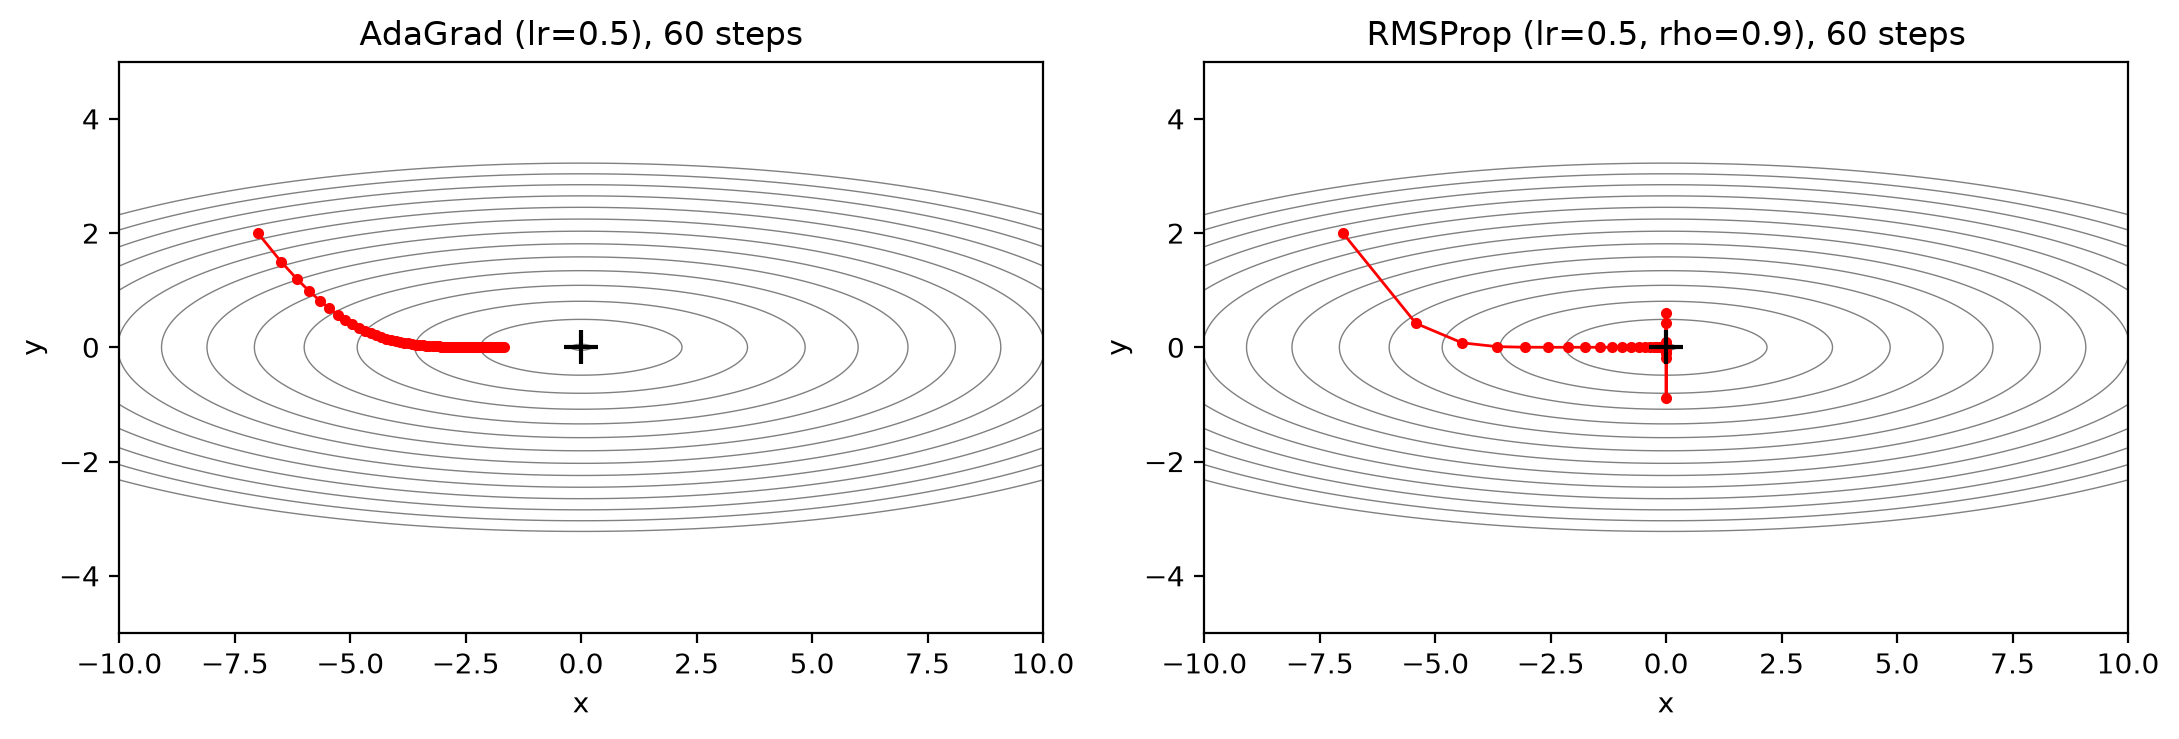
\includegraphics[width=\textwidth]{figures/opt_adagrad_rmsprop.png}

\small 같은 학습률 $\alpha=0.5$로 $60$단계: AdaGrad는 점점 느려져 멈추고, RMSProp은 최솟값 근처까지 간다.
\end{center}
}{%
\begin{center}
\fbox{\parbox{0.8\textwidth}{\centering\small
[그림 자리] \texttt{figures/opt\_adagrad\_rmsprop.png}\\
\texttt{optimizers\_2d.py}를 실행하면 생성된다.}}
\end{center}
}

RMSProp의 경로 끝에서 $y$가 $0$ 근처에서 위아래로 흔들리는 것도 보인다.
gradient를 그 크기로 나누면 gradient가 아주 작아져도 보폭이 대략 $\alpha$로 유지되기 때문이다.
그래서 실제 학습에서는 학습이 진행될수록 학습률을 줄이기도 한다.

% -------------------------------------------------
\subsection{Adam}\label{sec:adam}
% -------------------------------------------------

\paragraph{아이디어: 모멘텀 + RMSProp.}
모멘텀은 \textbf{방향}을, RMSProp은 \textbf{매개변수별 보폭}을 개선하였다.
Adam(Adaptive Moment Estimation)은 두 가지를 합친 방법이다.
gradient의 지수이동평균 $m$ (모멘텀의 역할)과 gradient 제곱의 지수이동평균 $v$ (RMSProp의 역할)를 함께 사용한다.

\paragraph{갱신 규칙.}
$k=1,2,\ldots$번째 갱신에서 ($g_k$는 $W_{k-1}$에서의 gradient, $m_0=v_0=0$)
\[
\boxed{
\begin{aligned}
m_k&=\beta_1\,m_{k-1}+(1-\beta_1)\,g_k,
&\qquad
v_k&=\beta_2\,v_{k-1}+(1-\beta_2)\,g_k\odot g_k,\\[4pt]
\hat m_k&=\frac{m_k}{1-\beta_1^{\,k}},
&\qquad
\hat v_k&=\frac{v_k}{1-\beta_2^{\,k}},\\[4pt]
W_k&=W_{k-1}-\alpha\,\frac{\hat m_k}{\sqrt{\hat v_k}+\varepsilon}
\end{aligned}
}
\]
보통 $\beta_1=0.9$, $\beta_2=0.999$, $\varepsilon=10^{-8}$을 사용한다.
\begin{itemize}[leftmargin=1.8em]
\item $m$: gradient의 평균 $\approx$ ``어느 방향으로 가야 하는가'' (1차 moment)
\item $v$: gradient 제곱의 평균 $\approx$ ``이 매개변수의 gradient는 보통 얼마나 큰가'' (2차 moment)
\item $\hat m/\sqrt{\hat v}$: 평균 방향을 그 크기로 나누어, 매개변수마다 보폭을 비슷한 수준으로 맞춘다.
\end{itemize}

\paragraph{편향 보정 (bias correction).}
$m$과 $v$를 $0$에서 시작하므로 초기에는 실제 평균보다 작게 치우친다.
예를 들어 첫 단계에서 $m_1=(1-\beta_1)g_1=0.1\,g_1$로, 실제 gradient의 $\frac{1}{10}$밖에 되지 않는다.
이를 $1-\beta_1^{\,k}$로 나누면
\[
\hat m_1=\frac{0.1\,g_1}{1-0.9}=g_1
\]
로 바로잡힌다. $k$가 커지면 $\beta_1^{\,k}\to0$이므로 보정의 효과는 사라진다.
$v$도 같은 방식으로 보정한다.

\paragraph{예제: 첫 단계.}
편향 보정 덕분에 $\hat m_1=g_1$, $\hat v_1=g_1\odot g_1$이므로
\[
W_1=W_0-\alpha\frac{g_1}{|g_1|}
\]
이고, AdaGrad처럼 각 좌표가 정확히 $\alpha$만큼 움직인다.
$\alpha=0.3$이면 $(x_1,y_1)=(-6.7,\ 1.7)$이다.

\begin{lstlisting}
class Adam:
    """m <- b1*m + (1-b1)*g,   v <- b2*v + (1-b2)*g*g,
       W <- W - lr * m_hat / (sqrt(v_hat) + eps)   (m_hat, v_hat: bias-corrected)"""
    def __init__(self, lr=0.001, beta1=0.9, beta2=0.999, eps=1e-8):
        self.lr = lr
        self.beta1 = beta1
        self.beta2 = beta2
        self.eps = eps
        self.k = 0
        self.m = None
        self.v = None

    def update(self, params, grads):
        if self.m is None:
            self.m = {key: np.zeros_like(val) for key, val in params.items()}
            self.v = {key: np.zeros_like(val) for key, val in params.items()}
        self.k += 1
        for key in params:
            self.m[key] = self.beta1 * self.m[key] + (1 - self.beta1) * grads[key]
            self.v[key] = self.beta2 * self.v[key] + (1 - self.beta2) * grads[key] ** 2
            m_hat = self.m[key] / (1 - self.beta1 ** self.k)     # bias correction
            v_hat = self.v[key] / (1 - self.beta2 ** self.k)
            params[key] -= self.lr * m_hat / (np.sqrt(v_hat) + self.eps)
\end{lstlisting}

% -------------------------------------------------
\subsection{네 가지 기법의 비교}\label{sec:compare}
% -------------------------------------------------

같은 시작점 $(-7,2)$에서 $30$단계씩 갱신한 결과이다.
학습률은 각 기법이 잘 동작하도록 따로 정하였다
(SGD $0.95$, 모멘텀 $0.1$ ($\beta=0.9$), AdaGrad $1.5$, Adam $0.3$).

\begin{lstlisting}
optimizers = {
    "SGD (lr=0.95)":                SGD(lr=0.95),
    "Momentum (lr=0.1, beta=0.9)":  Momentum(lr=0.1, beta=0.9),
    "AdaGrad (lr=1.5)":             AdaGrad(lr=1.5),
    "Adam (lr=0.3)":                Adam(lr=0.3),
}
paths = {name: minimize(opt) for name, opt in optimizers.items()}
\end{lstlisting}

\IfFileExists{figures/opt_compare.png}{%
\begin{center}
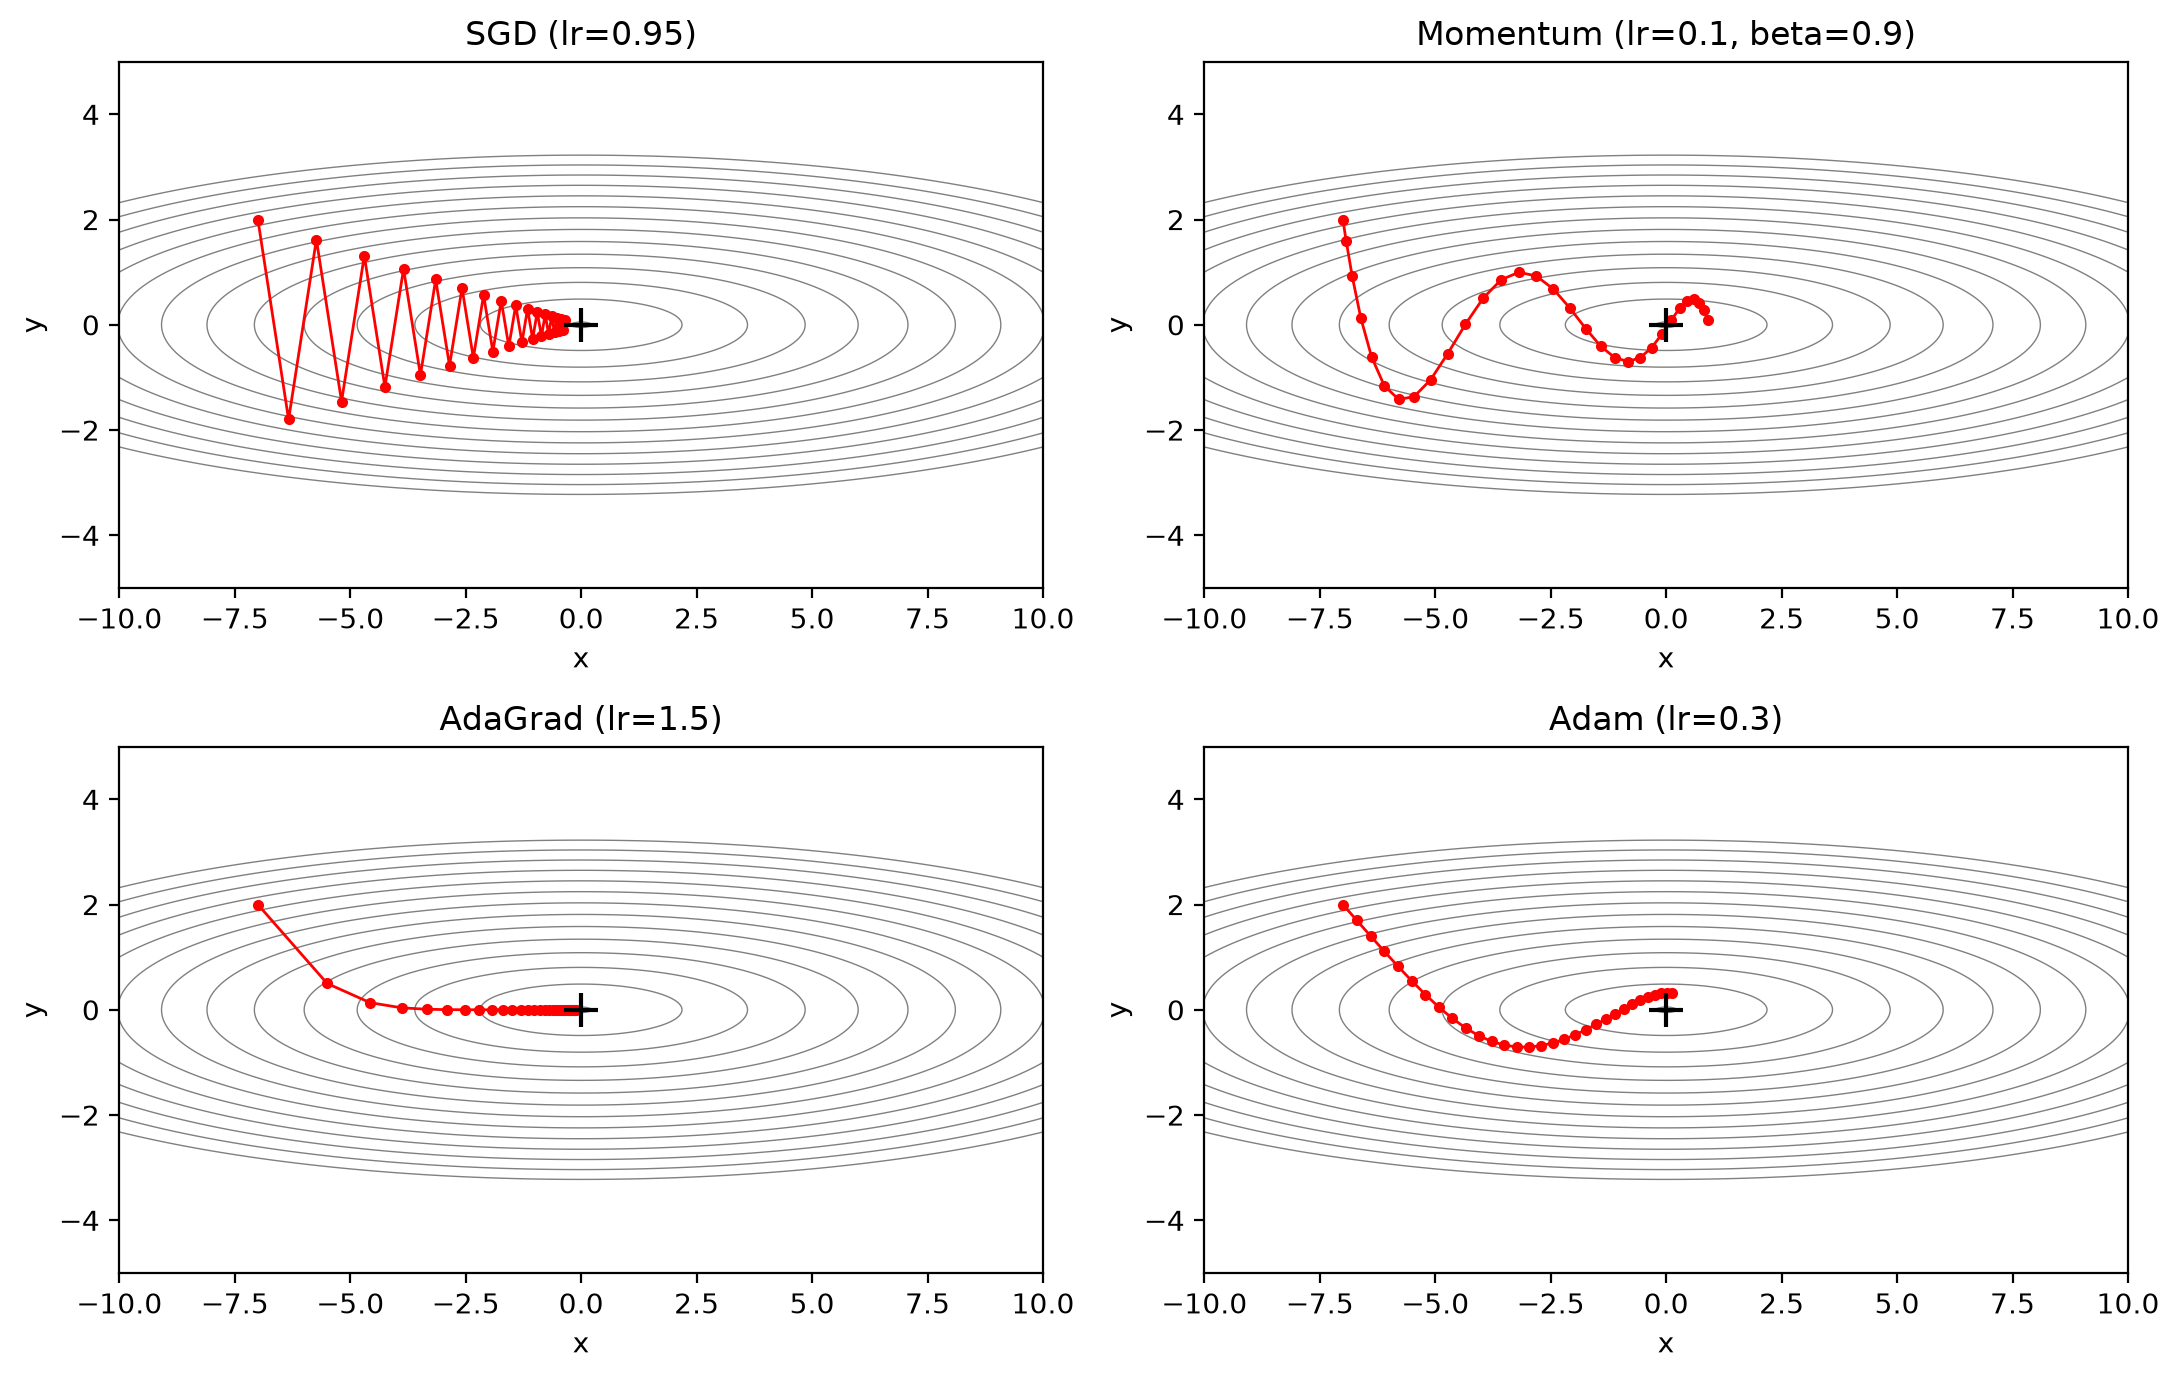
\includegraphics[width=\textwidth]{figures/opt_compare.png}

\small 네 가지 최적화 기법의 경로 ($+$: 최솟값 $(0,0)$)
\end{center}
}{%
\begin{center}
\fbox{\parbox{0.8\textwidth}{\centering\small
[그림 자리] \texttt{figures/opt\_compare.png}\\
\texttt{optimizers\_2d.py}를 실행하면 생성된다.}}
\end{center}
}

\IfFileExists{figures/opt_loss.png}{%
\begin{center}
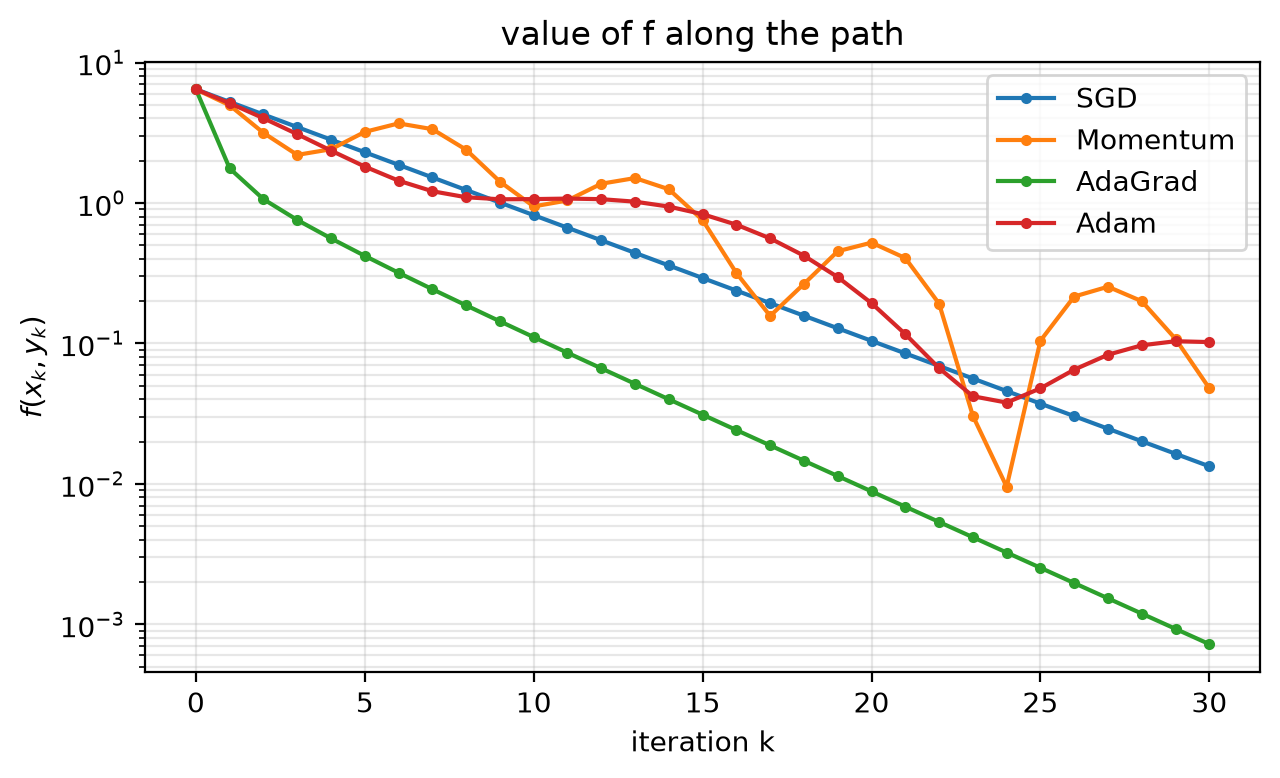
\includegraphics[width=0.7\textwidth]{figures/opt_loss.png}

\small 경로를 따라 계산한 $f(x_k,y_k)$ (세로축은 로그 눈금)
\end{center}
}{%
\begin{center}
\fbox{\parbox{0.8\textwidth}{\centering\small
[그림 자리] \texttt{figures/opt\_loss.png}\\
\texttt{optimizers\_2d.py}를 실행하면 생성된다.}}
\end{center}
}

\begin{center}
\begin{tabular}{@{}llp{0.42\textwidth}@{}}
\toprule
기법 & 첫 두 단계 $(x_1,y_1)$, $(x_2,y_2)$ & 경로의 특징 \\
\midrule
SGD & $(-6.335,\,-1.8)$, $(-5.733,\,1.62)$ & $y$ 방향으로 지그재그, $x$ 방향은 느림 \\
모멘텀 & $(-6.93,\,1.6)$, $(-6.798,\,0.92)$ & 공이 굴러가듯 크게 휘며 가속, 최솟값을 지나쳤다 돌아옴 \\
AdaGrad & $(-5.5,\,0.5)$, $(-4.573,\,0.136)$ & $y$ 진동을 바로 잡고 골짜기 바닥을 따라 곧게 이동 \\
Adam & $(-6.7,\,1.7)$, $(-6.400,\,1.402)$ & 모멘텀처럼 휘지만 진동이 훨씬 작음 \\
\bottomrule
\end{tabular}
\end{center}

\begin{keybox}[매개변수 갱신 기법 정리]
\begin{center}
\begin{tabular}{@{}lll@{}}
\toprule
기법 & 갱신 규칙 & 개선한 점 \\
\midrule
SGD & $W\leftarrow W-\alpha g$ & (기준) \\[3pt]
모멘텀 & $v\leftarrow\beta v-\alpha g,\ \ W\leftarrow W+v$ & 방향: 진동 상쇄, 가속 \\[3pt]
AdaGrad & $h\leftarrow h+g\odot g,\ \ W\leftarrow W-\alpha\,g/\sqrt h$ & 보폭: 매개변수별 학습률 \\[3pt]
RMSProp & $h\leftarrow\rho h+(1-\rho)g\odot g,\ \ W\leftarrow W-\alpha\,g/\sqrt h$ & 학습률이 $0$으로 줄지 않음 \\[3pt]
Adam & $m$, $v$의 지수이동평균 + 편향 보정 & 모멘텀 + RMSProp \\
\bottomrule
\end{tabular}
\end{center}
\end{keybox}

\begin{remarkbox}[어떤 기법이 가장 좋은가?]
이 예제에서는 AdaGrad가 가장 빨리 수렴하였지만, 이것으로 순위를 정할 수는 없다.
결과는 함수의 모양, 시작점, 학습률 같은 hyper-parameter에 따라 크게 달라진다.
실제 딥러닝에서는 Adam이 hyper-parameter에 덜 민감하여 기본값으로 많이 쓰이고,
잘 조정한 SGD (+ 모멘텀)가 최종 성능이 더 좋은 경우도 많다.
PyTorch에서는 \texttt{torch.optim.SGD(..., momentum=0.9)}, \texttt{torch.optim.Adagrad},
\texttt{torch.optim.RMSprop}, \texttt{torch.optim.Adam}으로 제공된다.
\end{remarkbox}

\begin{thinkbox}[생각해 보자]
\begin{itemize}[leftmargin=1.5em]
\item SGD에서 $\alpha=0.5$일 때 $y$는 한 번에 $0$이 되었다. $x$가 한 번에 $0$이 되는 학습률은 얼마인가?
그 학습률로 갱신하면 $y$는 어떻게 되는가?
\item 모멘텀에서 $\beta$를 $0.5$, $0.99$로 바꾸면 경로가 어떻게 달라질까?
(\texttt{optimizers\_2d.py}에서 직접 확인해 보라.)
\item AdaGrad와 Adam은 첫 단계에서 gradient의 크기와 관계없이 각 좌표를 $\alpha$만큼 움직였다.
이것은 장점인가, 단점인가?
\item 함수를 $f(x,y)=x^2+y^2$ (곡률이 같은 경우)로 바꾸면 SGD와 다른 기법의 차이는 어떻게 될까?
\end{itemize}
\end{thinkbox}

% -------------------------------------------------
\subsection{MNIST에서의 비교}\label{sec:mnistopt}
% -------------------------------------------------

2변수 함수에서 본 차이가 실제 신경망 학습에서도 나타날까?
지난주 과제에서 사용한 심층신경망 \texttt{MultiLayerNet}
(은닉층 $4$개, 각 $100$개 node, ReLU, 가중치 초기화 표준편차 $0.05$)을
네 가지 optimizer로 학습시켜 비교하자.
공정한 비교를 위해 \textbf{같은 초기 가중치, 같은 미니배치 순서}를 사용하고,
\textbf{갱신 규칙 한 줄만} 바꾼다.
학습률은 각 기법에서 흔히 쓰는 값으로 정하였다.
\[
\text{SGD }0.01,\quad \text{모멘텀 }0.01,\quad \text{AdaGrad }0.01,\quad \text{Adam }0.001
\]

\begin{lstlisting}
optimizers = {
    "SGD":      SGD(lr=0.01),
    "Momentum": Momentum(lr=0.01, beta=0.9),
    "AdaGrad":  AdaGrad(lr=0.01),
    "Adam":     Adam(lr=0.001),
}
hidden = [100, 100, 100, 100]      # 4 hidden layers, 100 nodes each
epochs = 5
batch_size = 128

N = x_train.shape[0]
iter_per_epoch = N // batch_size

loss_hist = {}
val_hist = {}
for name, optimizer in optimizers.items():
    np.random.seed(1)                                   # the SAME initial weights for every optimizer
    net = MultiLayerNet(784, hidden, 10, activation="relu", loss="ce")
    np.random.seed(2)                                   # the SAME mini-batches for every optimizer
    loss_hist[name], val_hist[name] = [], []
    t0 = time.time()
    for epoch in range(epochs):
        perm = np.random.permutation(N)
        for it in range(iter_per_epoch):
            idx = perm[it * batch_size:(it + 1) * batch_size]
            loss = net.loss(x_train[idx], t_train[idx])
            grads = net.backward()
            optimizer.update(net.params, grads)         # <- the only line that differs
            loss_hist[name].append(loss)
        val_hist[name].append(net.accuracy(x_val, t_val))
\end{lstlisting}

전체 코드는 \texttt{mnist\_optimizer\_compare.py}에 있다.
데이터, network, optimizer는 모듈에서 불러온다.
\begin{lstlisting}
from mnist_data import load_mnist_split
from layers import MultiLayerNet
from optimizers import SGD, Momentum, AdaGrad, Adam
\end{lstlisting}
\texttt{layers.py}의 계층과 \texttt{MultiLayerNet}은 지난주 \texttt{mnist\_mlp.py}와 똑같고,
\texttt{load\_mnist\_split()}은 지난주와 같은 훈련/검증 분할을 돌려준다.

\IfFileExists{figures/mnist_optimizers.png}{%
\begin{center}
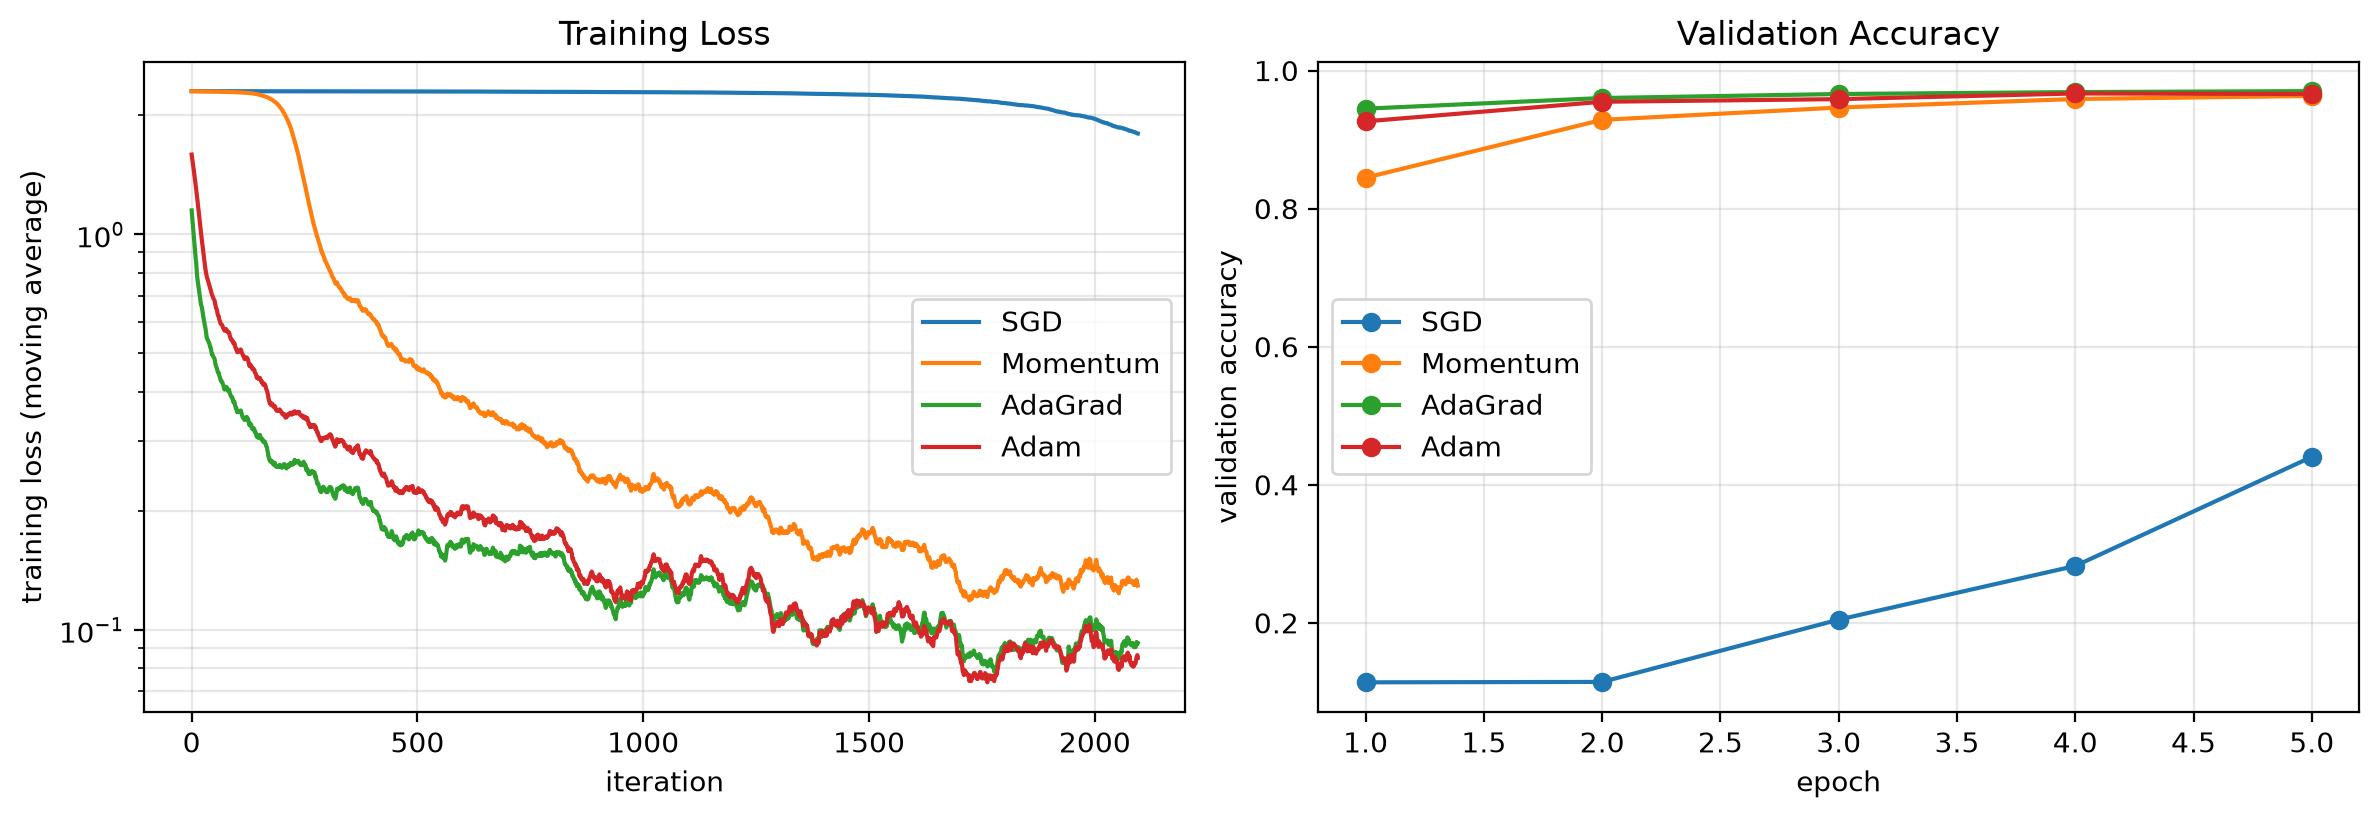
\includegraphics[width=\textwidth]{figures/mnist_optimizers.png}

\small iteration에 따른 훈련 손실 (50 iteration 이동평균, 로그 눈금, 왼쪽)과 epoch별 검증 정확도 (오른쪽)
\end{center}
}{%
\begin{center}
\fbox{\parbox{0.8\textwidth}{\centering\small
[그림 자리] \texttt{figures/mnist\_optimizers.png}\\
\texttt{mnist\_optimizer\_compare.py}를 실행하면 생성된다.}}
\end{center}
}

\begin{center}
\begin{tabular}{@{}lccccc@{}}
\toprule
& \multicolumn{5}{c}{검증 정확도} \\
\cmidrule(l){2-6}
optimizer & 1 epoch & 2 epoch & 3 epoch & 4 epoch & 5 epoch \\
\midrule
SGD ($0.01$) & $11.4\%$ & $11.4\%$ & $20.5\%$ & $28.2\%$ & $44.0\%$ \\
모멘텀 ($0.01$) & $84.5\%$ & $92.9\%$ & $94.6\%$ & $95.9\%$ & $96.3\%$ \\
AdaGrad ($0.01$) & $94.5\%$ & $96.0\%$ & $96.6\%$ & $96.9\%$ & $97.0\%$ \\
Adam ($0.001$) & $92.6\%$ & $95.5\%$ & $95.9\%$ & $96.7\%$ & $96.6\%$ \\
\bottomrule
\end{tabular}
\end{center}

\begin{itemize}[leftmargin=1.8em]
\item \textbf{SGD}: 처음 $1800$ iteration 가까이 손실이 $\log10\approx2.30$ 근처에서 거의 줄지 않는다.
손실이 거의 평평한 구간(\textbf{plateau})에 머물러 gradient가 아주 작기 때문이다.
$10$개 class를 모두 $\frac{1}{10}$의 확률로 찍는 상태가 손실 $\log10$이다.
\item \textbf{모멘텀}: 처음에는 SGD처럼 멈춰 있다가, 약 $200$ iteration 뒤에 plateau를 빠져나온다.
같은 방향의 작은 gradient가 속도에 \textbf{누적}되어 보폭이 점점 커졌기 때문이다
(\ref{sec:momentum}절: 최대 $\frac{1}{1-\beta}=10$배).
\item \textbf{AdaGrad, Adam}: 처음부터 빠르게 내려간다.
gradient를 그 크기로 나누므로, gradient가 아주 작은 plateau에서도 보폭이 대략 $\alpha$ 수준으로 유지된다
(\ref{sec:adagrad}절: 첫 단계에서 각 좌표가 gradient의 크기와 관계없이 $\alpha$만큼 움직였던 것).
\end{itemize}

\begin{remarkbox}[이 결과를 어떻게 읽어야 할까?]
SGD가 느렸던 것은 SGD 자체가 나빠서라기보다,
\textbf{깊은 network와 작은 초기 가중치} 때문에 처음 gradient가 매우 작은 상황에서
학습률 $0.01$이 너무 작았기 때문이다.
학습률을 키우거나(연습문제 5), 가중치를 더 잘 초기화하면 SGD도 잘 학습한다.
초기 가중치가 학습에 주는 영향은 다음 절 \textbf{가중치의 초깃값}에서 자세히 다룬다.
또 $5$ epoch 뒤의 검증 정확도는 모멘텀, AdaGrad, Adam이 모두 $96\sim97\%$로 비슷하다.
optimizer의 차이는 주로 \textbf{얼마나 빨리, 얼마나 안정적으로} 학습하는가에서 나타난다.
\end{remarkbox}

% =================================================
\section{가중치의 초깃값}\label{sec:init}
% =================================================

\ref{sec:mnistopt}절에서 SGD가 처음 $1800$ iteration 가까이 거의 학습하지 못한 것은,
깊은 network의 \textbf{작은 초기 가중치} 때문에 gradient가 아주 작았기 때문이었다.
학습은 초기 가중치에서 출발하므로, \textbf{어디서 출발하느냐}가 학습의 속도와 성패를 크게 좌우한다.
이 절에서는 초기 가중치를 어떻게 정해야 하는지 살펴본다.

\subsection{모든 가중치를 같은 값으로 두면?}

가장 먼저 떠오르는 방법은 모든 가중치를 $0$ (또는 같은 값)으로 두는 것이다.
그런데 은닉층의 가중치가 모두 같으면, 은닉층의 node들은 같은 입력에 같은 가중치를 곱하므로
\textbf{모두 같은 값}을 출력한다.
역전파에서도 이 node들은 대칭적인 위치에 있으므로 \textbf{같은 gradient}를 받고,
같은 양만큼 갱신된다. 그러면 학습이 끝날 때까지 모든 node가 계속 같은 값을 가진다.
\[
W^{(1)}=\begin{pmatrix}c&c&\cdots&c\\ \vdots&&&\vdots\\ c&c&\cdots&c\end{pmatrix}
\ \Longrightarrow\
z_1=z_2=\cdots=z_m
\ \Longrightarrow\
\pd{L}{w_{i1}}=\pd{L}{w_{i2}}=\cdots=\pd{L}{w_{im}}
\]
node를 $100$개 두어도 사실상 \textbf{node 하나}와 같은 network가 되는 것이다.
이 \textbf{대칭성을 깨기 위해} 초기 가중치는 무작위로 정한다.
(편향 $B$는 $0$으로 두어도 가중치가 무작위이면 대칭이 깨지므로 보통 $0$으로 시작한다.)

그렇다면 무작위 값의 \textbf{크기}, 즉 표준편차는 얼마로 해야 할까?

\subsection{은닉층의 활성화값 분포 실험}

다음 실험으로 초기 가중치의 크기가 network 안의 값들에 어떤 영향을 주는지 보자.
\begin{itemize}[leftmargin=1.8em]
\item 입력: 표준정규분포를 따르는 $100$차원 데이터 $1000$개 ($X$: $1000\times100$)
\item network: node가 $100$개인 층 $5$개, 편향은 $0$, \textbf{학습은 하지 않고} 순전파만 한다.
\item 각 층의 활성화값 $Z$ (활성화 함수를 거친 값)의 \textbf{히스토그램}을 그린다.
\end{itemize}

\begin{lstlisting}
def forward_activations(activation, weight_std, n_layers=5, n_nodes=100, n_data=1000, seed=0):
    """Feed 1000 random inputs through n_layers layers; return the list of activations Z of each layer."""
    rng = np.random.default_rng(seed)
    X = rng.standard_normal((n_data, n_nodes))          # input data (1000, 100)
    Z = X
    activations = []
    for i in range(n_layers):
        n_in = Z.shape[1]
        std = weight_std(n_in) if callable(weight_std) else weight_std
        W = std * rng.standard_normal((n_in, n_nodes))  # (input nodes, output nodes)
        A = Z @ W                                       # bias = 0
        Z = activation(A)
        activations.append(Z)
    return activations
\end{lstlisting}
전체 코드는 \texttt{weight\_init\_activation.py}에 있다.

\paragraph{Sigmoid의 경우.}
가중치의 표준편차를 $1$, $0.01$, 그리고 뒤에서 설명할 Xavier 초깃값 $\frac{1}{\sqrt n}$
($n$: 앞 층의 node 수, 여기서는 $100$이므로 $0.1$)로 바꾸어 본다.

\IfFileExists{figures/init_sigmoid.png}{%
\begin{center}
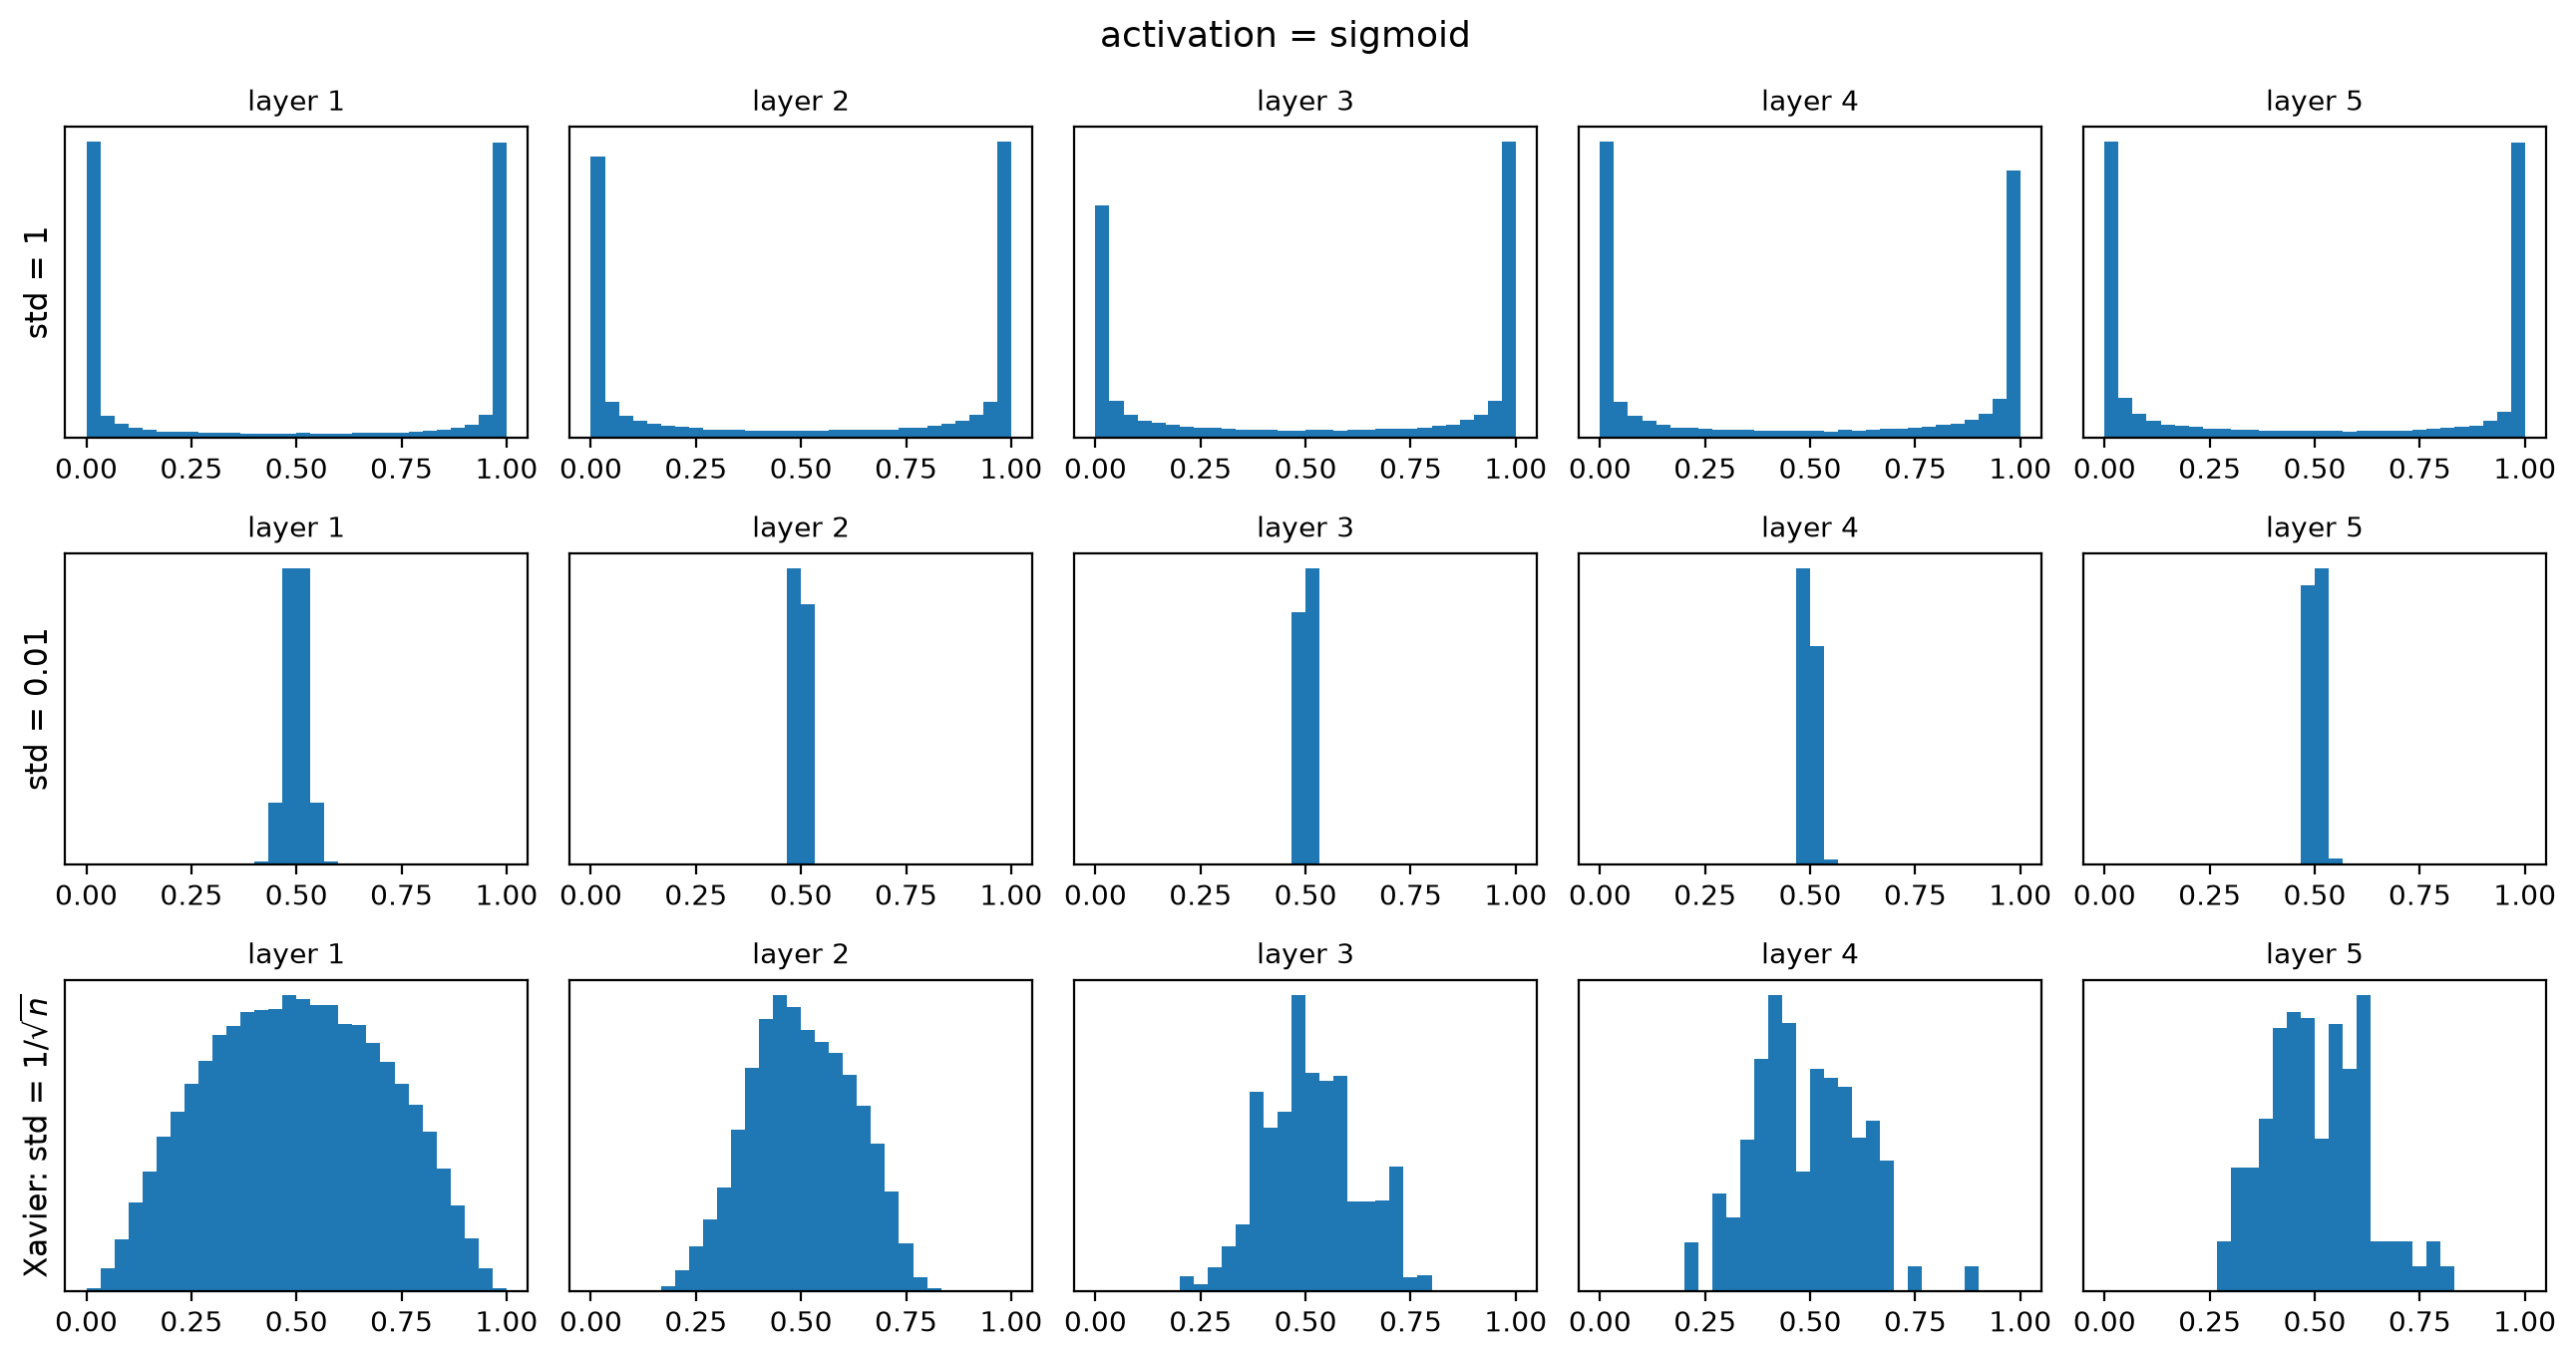
\includegraphics[width=\textwidth]{figures/init_sigmoid.png}

\small sigmoid를 쓴 $5$층 network에서 층별 활성화값의 분포
\end{center}
}{%
\begin{center}
\fbox{\parbox{0.8\textwidth}{\centering\small
[그림 자리] \texttt{figures/init\_sigmoid.png}\\
\texttt{weight\_init\_activation.py}를 실행하면 생성된다.}}
\end{center}
}

\begin{itemize}[leftmargin=1.8em]
\item \textbf{표준편차 $1$}: 활성화값이 $0$과 $1$에 몰려 있다.
가중치가 크면 $A=ZW$의 절댓값이 커져 sigmoid가 양 끝의 평평한 부분에 가기 때문이다.
그곳에서 sigmoid의 미분 $\sigma'(a)=z(1-z)$는 거의 $0$이다.
역전파에서 gradient는 층을 하나 지날 때마다 $\sigma'(a)$를 곱하므로 (지난주 활성화 계층의 역전파)
앞쪽 층으로 갈수록 gradient가 사라진다. 이를 \textbf{기울기 소실(vanishing gradient)}이라 한다.
\item \textbf{표준편차 $0.01$}: 활성화값이 모두 $0.5$ 근처에 모여 있다.
기울기 소실은 덜하지만, $100$개의 node가 거의 \textbf{같은 값}을 출력하므로
앞에서 본 대칭 문제와 비슷하게 node를 많이 둔 의미가 없어진다 (\textbf{표현력 제한}).
또 가중치가 작으면 역전파에서 $W\T$를 곱할 때마다 gradient도 작아진다.
\item \textbf{Xavier ($\frac{1}{\sqrt n}$)}: 층이 깊어져도 활성화값이 \textbf{적당히 퍼진} 분포를 유지한다.
\end{itemize}

뒤쪽 층에서 분포가 조금 좁아지고 울퉁불퉁해지는 것은
sigmoid의 출력이 $0$이 아니라 $0.5$를 중심으로 하기 때문이다.
원점에 대칭인 tanh를 쓰면 같은 Xavier 초깃값에서도 분포가 고르게 유지된다.

\IfFileExists{figures/init_tanh.png}{%
\begin{center}
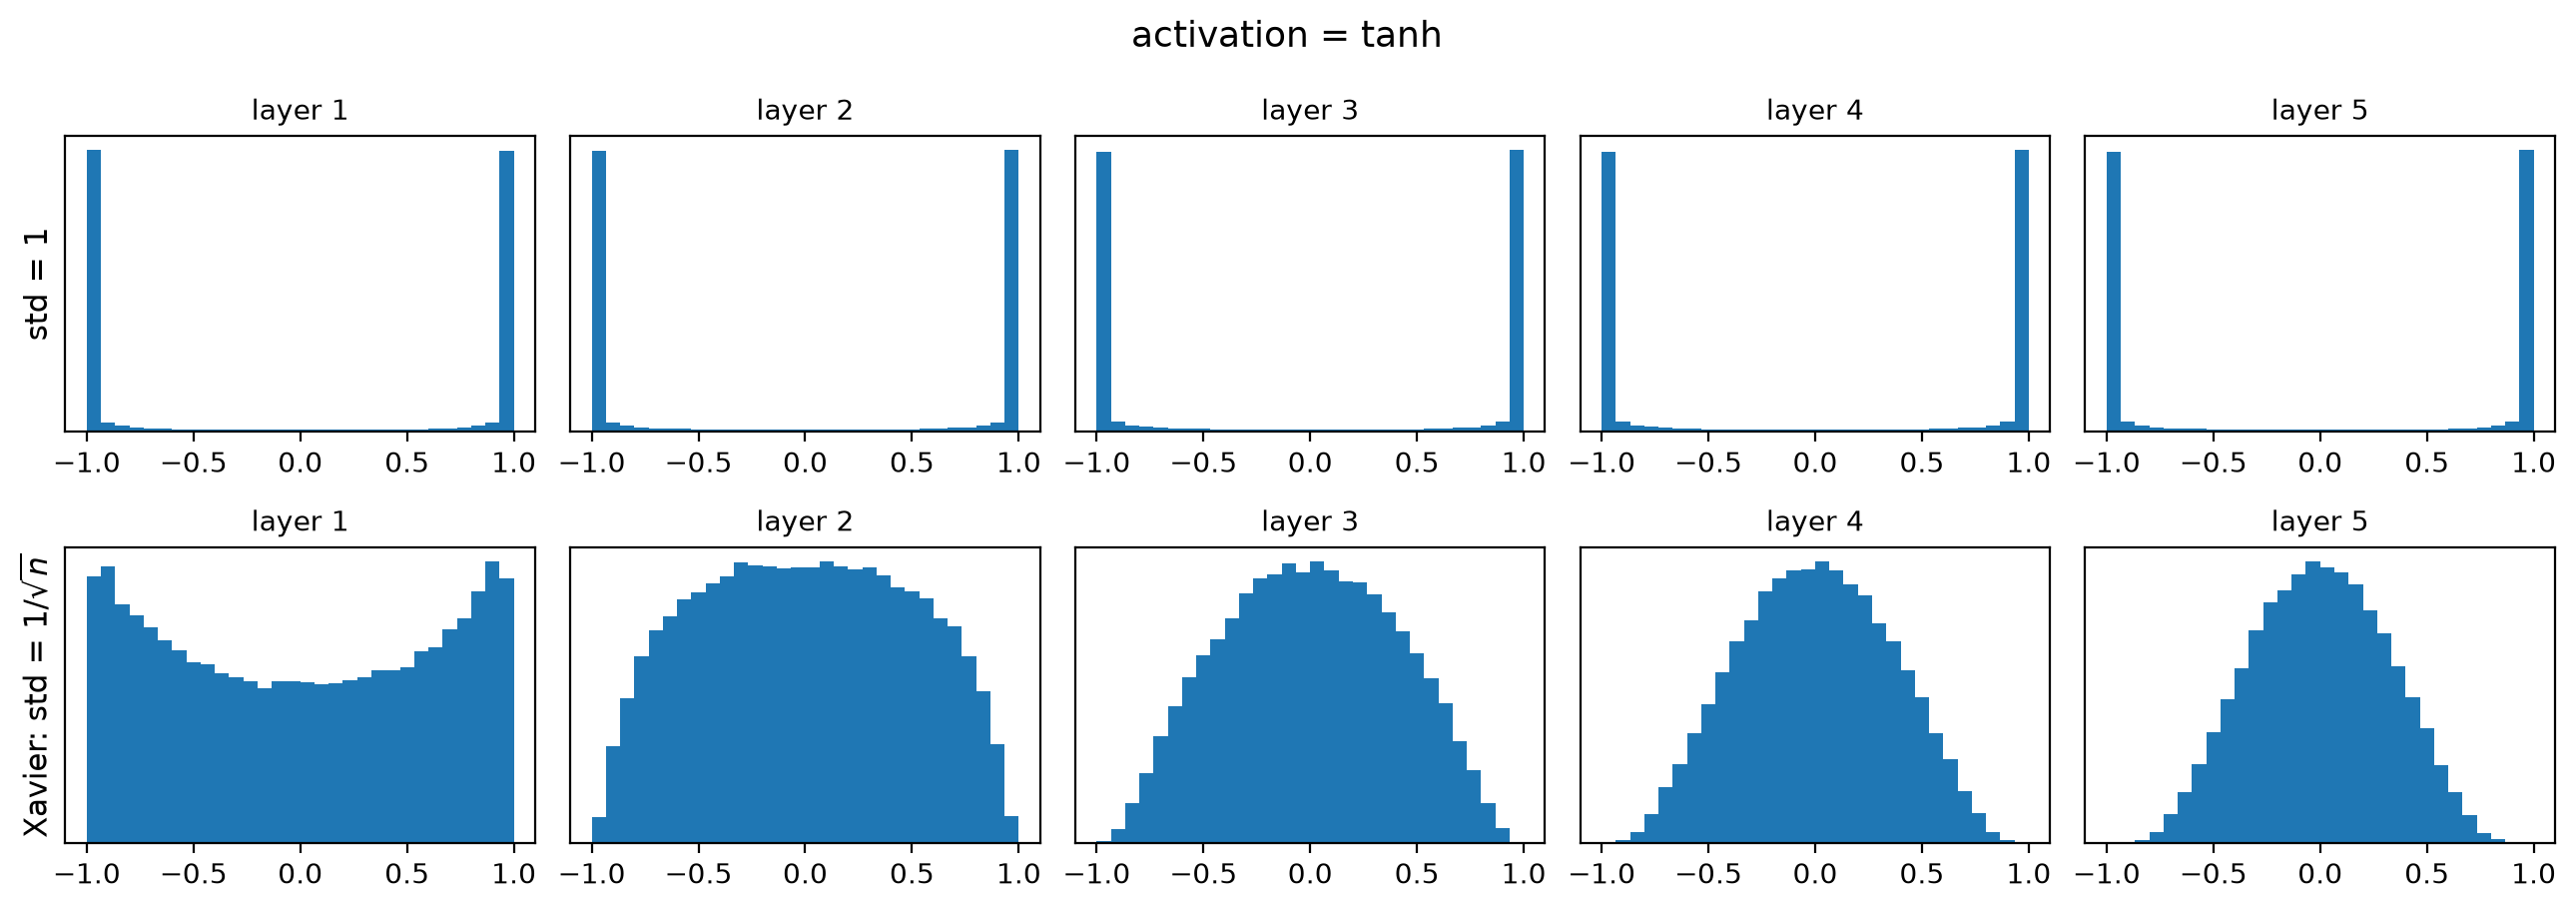
\includegraphics[width=\textwidth]{figures/init_tanh.png}

\small tanh를 쓴 경우: 표준편차 $1$이면 $\pm1$에 몰리고, Xavier 초깃값이면 고르게 퍼진다.
\end{center}
}{%
\begin{center}
\fbox{\parbox{0.8\textwidth}{\centering\small
[그림 자리] \texttt{figures/init\_tanh.png}\\
\texttt{weight\_init\_activation.py}를 실행하면 생성된다.}}
\end{center}
}

\begin{keybox}[활성화값 분포로 보는 좋은 초깃값]
각 층의 활성화값이 \textbf{적당히 퍼져 있어야} 한다.
\begin{itemize}[leftmargin=1.5em]
\item 양 끝에 몰리면 $\Rightarrow$ 활성화 함수의 미분이 $0$에 가까워 \textbf{기울기 소실}
\item 한 값에 몰리면 $\Rightarrow$ node들이 같은 값을 내어 \textbf{표현력 제한}
\end{itemize}
층마다 값의 크기(분산)가 \textbf{일정하게 유지}되도록 가중치의 표준편차를 정하면 된다.
\end{keybox}

\subsection{Xavier 초깃값}\label{sec:xavier}

층을 지날 때 분산이 일정하게 유지되려면 가중치의 분산이 얼마여야 할까?
앞 층의 node가 $n$개이고, 다음 층의 한 node의 입력이
\[
a_j=\sum_{i=1}^{n}z_i\,w_{ij}
\]
라 하자. 다음을 가정한다.
\begin{itemize}[leftmargin=1.8em]
\item $w_{ij}$들은 서로 독립이고 평균이 $0$, 분산이 $\mathrm{Var}(w)$인 같은 분포를 따른다.
\item $z_i$들도 서로 독립이고 평균이 $0$, 분산이 $\mathrm{Var}(z)$이며, 가중치와 독립이다.
\end{itemize}
독립인 확률변수의 합의 분산은 분산의 합이고, 평균이 $0$인 독립 확률변수의 곱은
$\mathrm{Var}(zw)=\mathbb E[z^2]\,\mathbb E[w^2]=\mathrm{Var}(z)\,\mathrm{Var}(w)$이므로
\[
\mathrm{Var}(a_j)=\sum_{i=1}^{n}\mathrm{Var}(z_i\,w_{ij})=n\,\mathrm{Var}(w)\,\mathrm{Var}(z)
\]
이다. 활성화 함수가 원점 근처에서 거의 항등함수라면 (tanh: $\tanh a\approx a$)
다음 층의 활성화값의 분산도 대략 $n\,\mathrm{Var}(w)\,\mathrm{Var}(z)$이다.
층을 지나도 분산이 변하지 않으려면 $n\,\mathrm{Var}(w)=1$, 즉
\[
\boxed{
\mathrm{Var}(w)=\frac{1}{n},
\qquad
\text{표준편차 }\frac{1}{\sqrt n}
\qquad(\text{Xavier 초깃값})
}
\]
이다. 앞 층의 node가 많을수록 가중치를 작게 해야 한다.

\begin{remarkbox}[Glorot와 Bengio의 원래 제안]
Xavier 초깃값은 Xavier Glorot와 Yoshua Bengio(2010)가 제안하여 \textbf{Glorot 초깃값}이라고도 한다.
같은 논리를 역전파에도 적용하면, gradient가 층을 거꾸로 지날 때 분산이 유지되려면
$\mathrm{Var}(w)=\frac{1}{n_{\mathrm{out}}}$ (다음 층의 node 수)이어야 한다.
원래 논문은 두 조건의 절충으로
\[
\mathrm{Var}(w)=\frac{2}{n_{\mathrm{in}}+n_{\mathrm{out}}}
\]
를 제안하였다. 앞뒤 층의 node 수가 같으면 $\frac1n$과 같다.
균등분포로 뽑을 때는 $\mathcal U\!\left(-\sqrt{\frac{6}{n_{\mathrm{in}}+n_{\mathrm{out}}}},\ \sqrt{\frac{6}{n_{\mathrm{in}}+n_{\mathrm{out}}}}\right)$를 쓴다
(구간 $[-r,r]$의 균등분포의 분산은 $\frac{r^2}{3}$).
\end{remarkbox}

\subsection{He 초깃값}\label{sec:he}

Xavier 초깃값은 활성화 함수가 원점 근처에서 선형이고 원점에 대칭이라는 가정에서 나왔다.
ReLU는 이 가정을 만족하지 않는다. ReLU는 \textbf{음수인 입력을 모두 $0$으로} 만들기 때문이다.

$a$가 평균 $0$인 대칭 분포를 따르면 절반은 양수, 절반은 음수이므로, $z=\max(0,a)$에 대해
\[
\mathbb E[z^2]=\frac12\,\mathbb E[a^2]=\frac12\,\mathrm{Var}(a)
\]
이다. ReLU를 지날 때마다 신호의 크기(제곱의 평균)가 \textbf{절반}으로 줄어드는 것이다.
다음 층의 입력은 (가중치의 평균이 $0$이므로)
\[
\mathrm{Var}\bigl(a^{(\ell+1)}\bigr)=n\,\mathrm{Var}(w)\,\mathbb E\bigl[z^2\bigr]
=n\,\mathrm{Var}(w)\cdot\frac12\,\mathrm{Var}\bigl(a^{(\ell)}\bigr)
\]
이다. ($z$의 평균이 $0$이 아니므로 $\mathrm{Var}(z)$ 대신 $\mathbb E[z^2]$가 들어간다.)
분산이 유지되려면 $\frac n2\,\mathrm{Var}(w)=1$, 즉
\[
\boxed{
\mathrm{Var}(w)=\frac{2}{n},
\qquad
\text{표준편차 }\sqrt{\frac{2}{n}}
\qquad(\text{He 초깃값})
}
\]
이다. ReLU가 절반을 버리는 만큼 Xavier 초깃값보다 분산을 \textbf{두 배}로 키운 것이다
(Kaiming He 등, 2015. \textbf{Kaiming 초깃값}이라고도 한다).

\paragraph{ReLU에서의 실험.}
ReLU를 쓴 $5$층 network에서 표준편차 $0.01$, Xavier, He를 비교하면 다음과 같다.
(ReLU는 약 절반의 값이 정확히 $0$이므로, $0$이 아닌 값만 그렸다.)

\IfFileExists{figures/init_relu.png}{%
\begin{center}
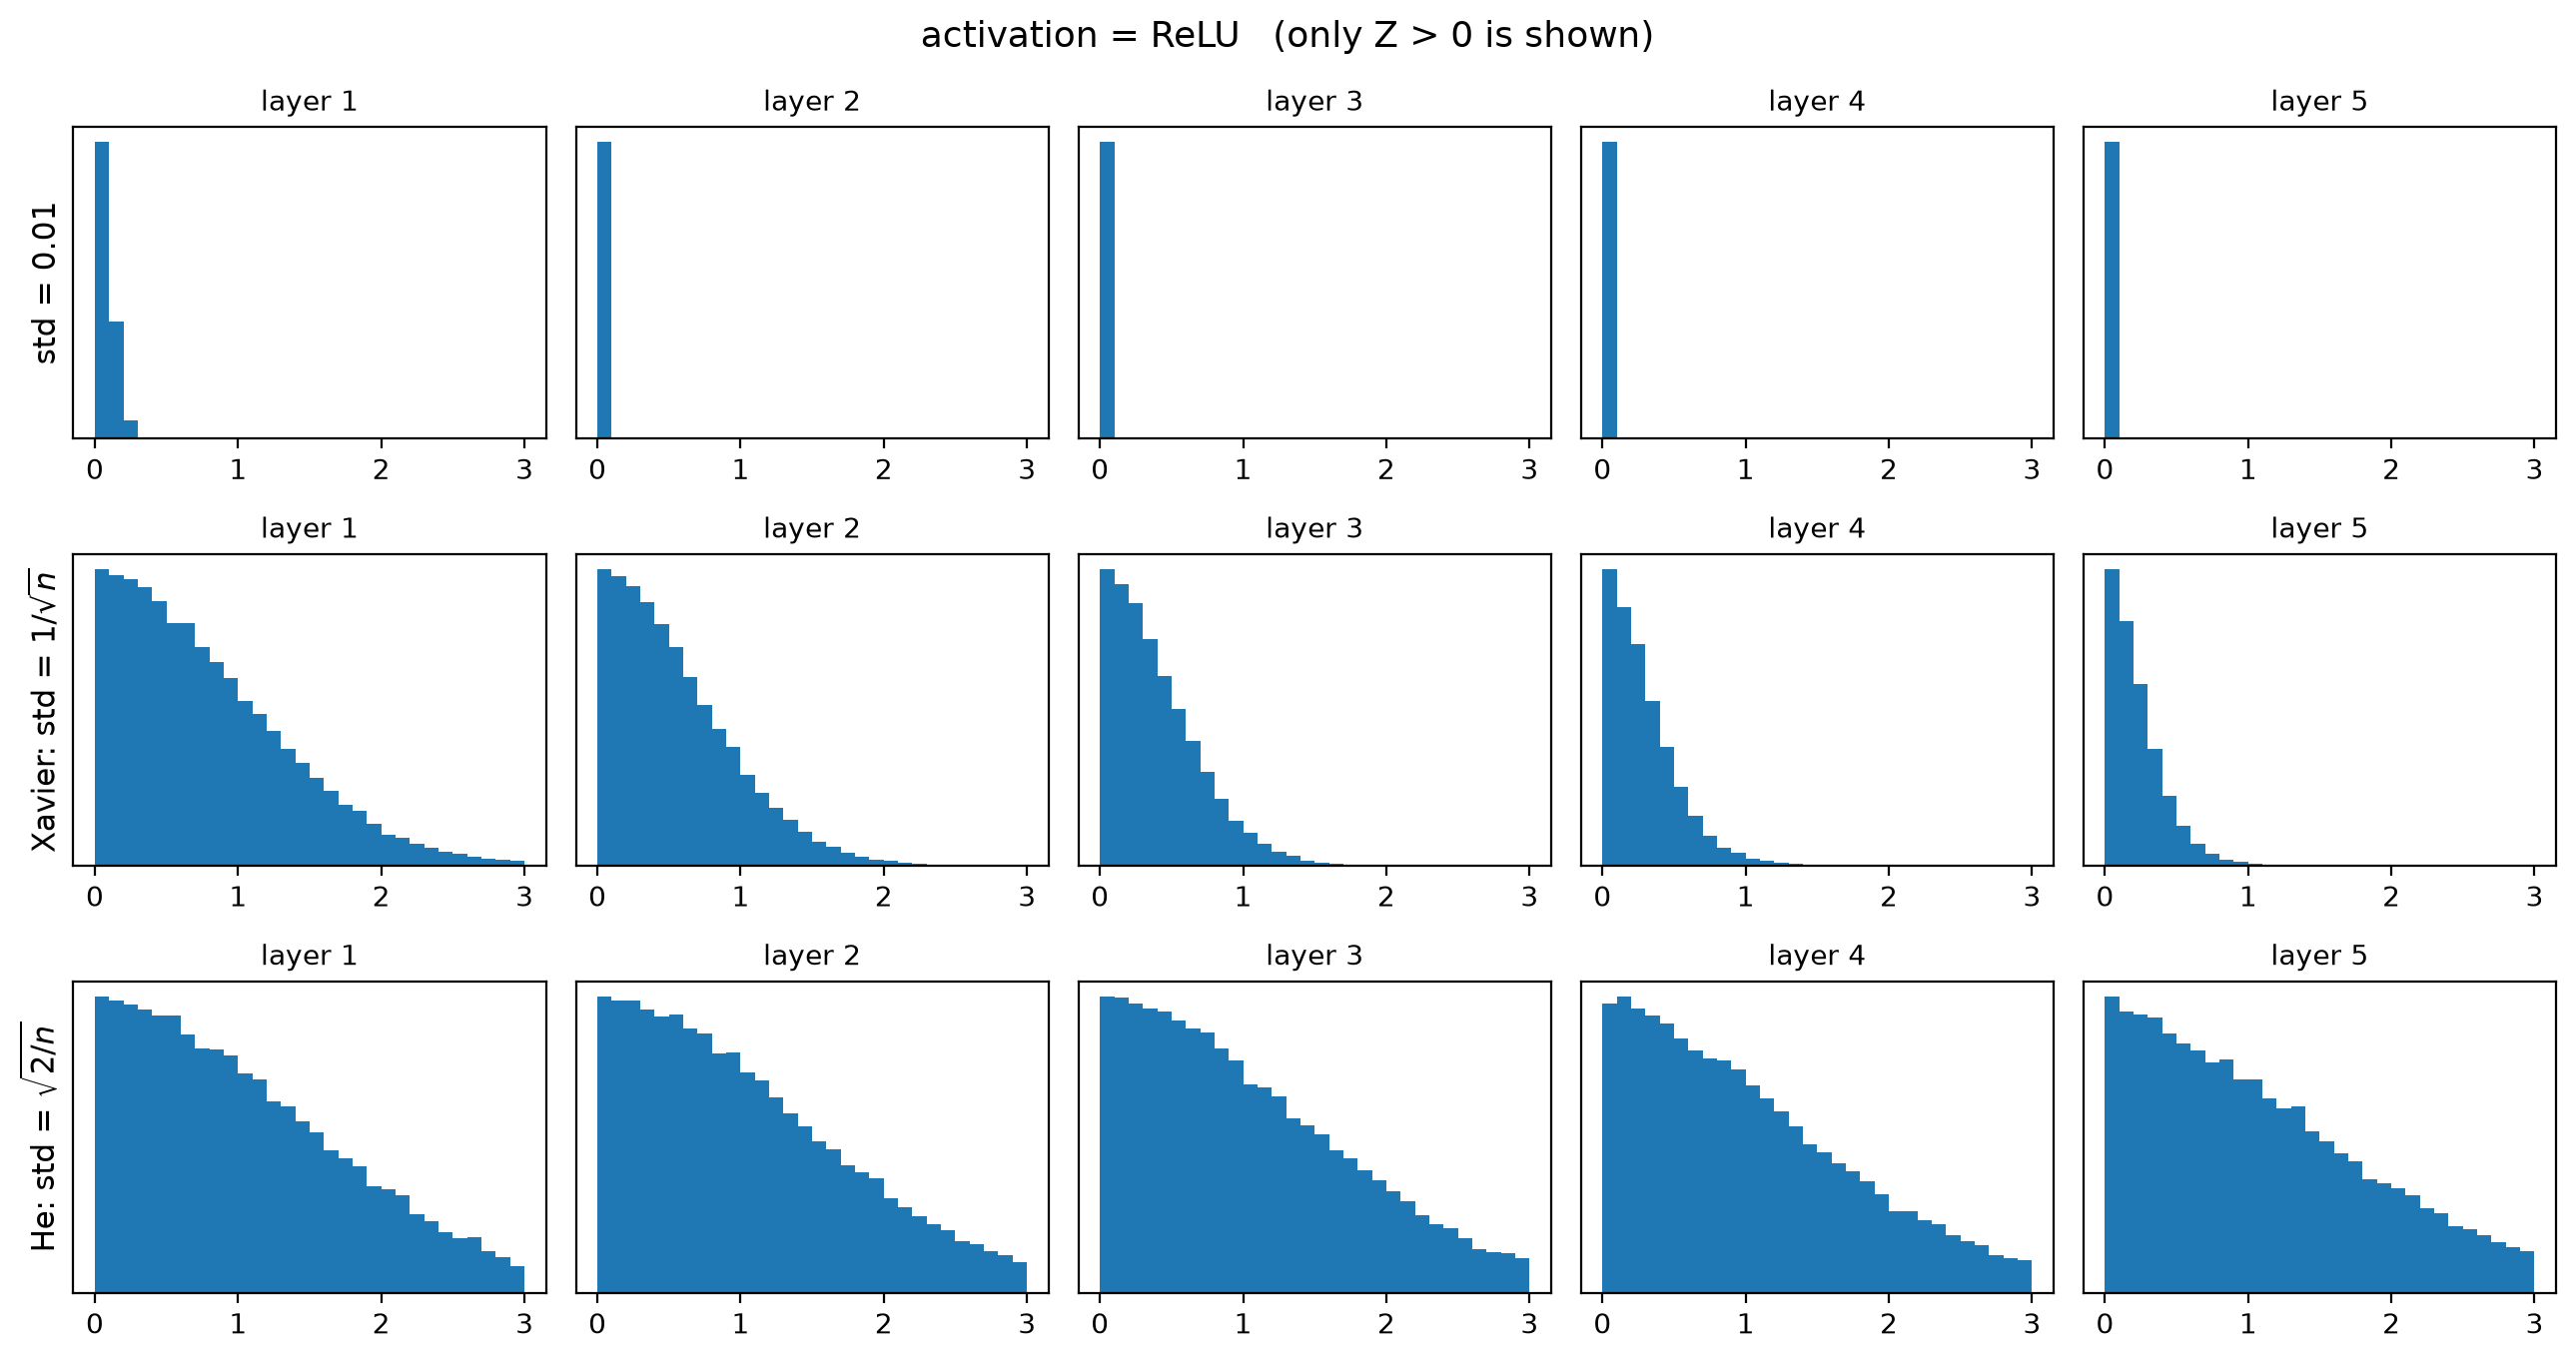
\includegraphics[width=\textwidth]{figures/init_relu.png}

\small ReLU를 쓴 $5$층 network에서 층별 활성화값의 분포 ($Z>0$인 값만)
\end{center}
}{%
\begin{center}
\fbox{\parbox{0.8\textwidth}{\centering\small
[그림 자리] \texttt{figures/init\_relu.png}\\
\texttt{weight\_init\_activation.py}를 실행하면 생성된다.}}
\end{center}
}

\begin{center}
\begin{tabular}{@{}lccccc@{}}
\toprule
& \multicolumn{5}{c}{층별 활성화값의 표준편차} \\
\cmidrule(l){2-6}
초깃값 & 1층 & 2층 & 3층 & 4층 & 5층 \\
\midrule
표준편차 $0.01$ & $0.058$ & $0.004$ & $0.0003$ & $0.0000$ & $0.0000$ \\
Xavier $\frac{1}{\sqrt n}$ & $0.58$ & $0.41$ & $0.30$ & $0.22$ & $0.18$ \\
He $\sqrt{\frac2n}$ & $0.82$ & $0.82$ & $0.86$ & $0.88$ & $1.00$ \\
\bottomrule
\end{tabular}
\end{center}

\begin{itemize}[leftmargin=1.8em]
\item \textbf{표준편차 $0.01$}: 층을 지날 때마다 값이 약 $\frac{1}{14}$로 줄어 $4$층부터는 사실상 $0$이다.
순전파의 신호가 사라지면 역전파의 gradient도 사라진다.
\item \textbf{Xavier}: ReLU가 매번 신호의 절반을 버리므로 층마다 약 $\frac{1}{\sqrt2}\approx0.71$배로 줄어든다.
층이 수십 개가 되면 결국 사라진다.
\item \textbf{He}: 층이 깊어져도 분포가 \textbf{거의 일정하게} 유지된다.
\end{itemize}

\begin{keybox}[초깃값 정리]
\begin{center}
\begin{tabular}{@{}lll@{}}
\toprule
활성화 함수 & 권장 초깃값 & 가중치의 표준편차 \\
\midrule
sigmoid, tanh & Xavier (Glorot) & $\sqrt{1/n}$ \ \ (또는 $\sqrt{2/(n_{\mathrm{in}}+n_{\mathrm{out}})}$) \\
ReLU 계열 & He (Kaiming) & $\sqrt{2/n}$ \\
\bottomrule
\end{tabular}
\end{center}
$n$은 앞 층의 node 수 (가중치 행렬 $W$의 행의 수, 입력 node 수)이다.
\end{keybox}

\subsection{MNIST에서의 비교}\label{sec:mnistinit}

\texttt{layers.py}의 \texttt{MultiLayerNet}이 \texttt{weight\_init\_std}에 숫자뿐 아니라
\texttt{"xavier"}, \texttt{"he"}도 받도록 고쳤다.
\begin{lstlisting}
            if weight_init_std == "xavier":            # Var(W) = 1/n_in  (sigmoid, tanh)
                std = np.sqrt(1.0 / n_in)
            elif weight_init_std == "he":              # Var(W) = 2/n_in  (ReLU)
                std = np.sqrt(2.0 / n_in)
            else:                                      # a fixed number, e.g. 0.01
                std = weight_init_std
            W = std * np.random.randn(n_in, n_out)     # (input nodes, output nodes)
\end{lstlisting}

은닉층 $5$개 (각 $100$개 node, ReLU)인 network를 \textbf{같은 SGD} (학습률 $0.01$)로 학습시키고,
초깃값만 바꾸어 비교한다 (\texttt{mnist\_init\_compare.py}).
\begin{lstlisting}
inits = {
    "std = 0.01": 0.01,
    "Xavier":     "xavier",
    "He":         "he",
}
hidden = [100, 100, 100, 100, 100]      # 5 hidden layers, 100 nodes each
\end{lstlisting}

\IfFileExists{figures/mnist_init.png}{%
\begin{center}
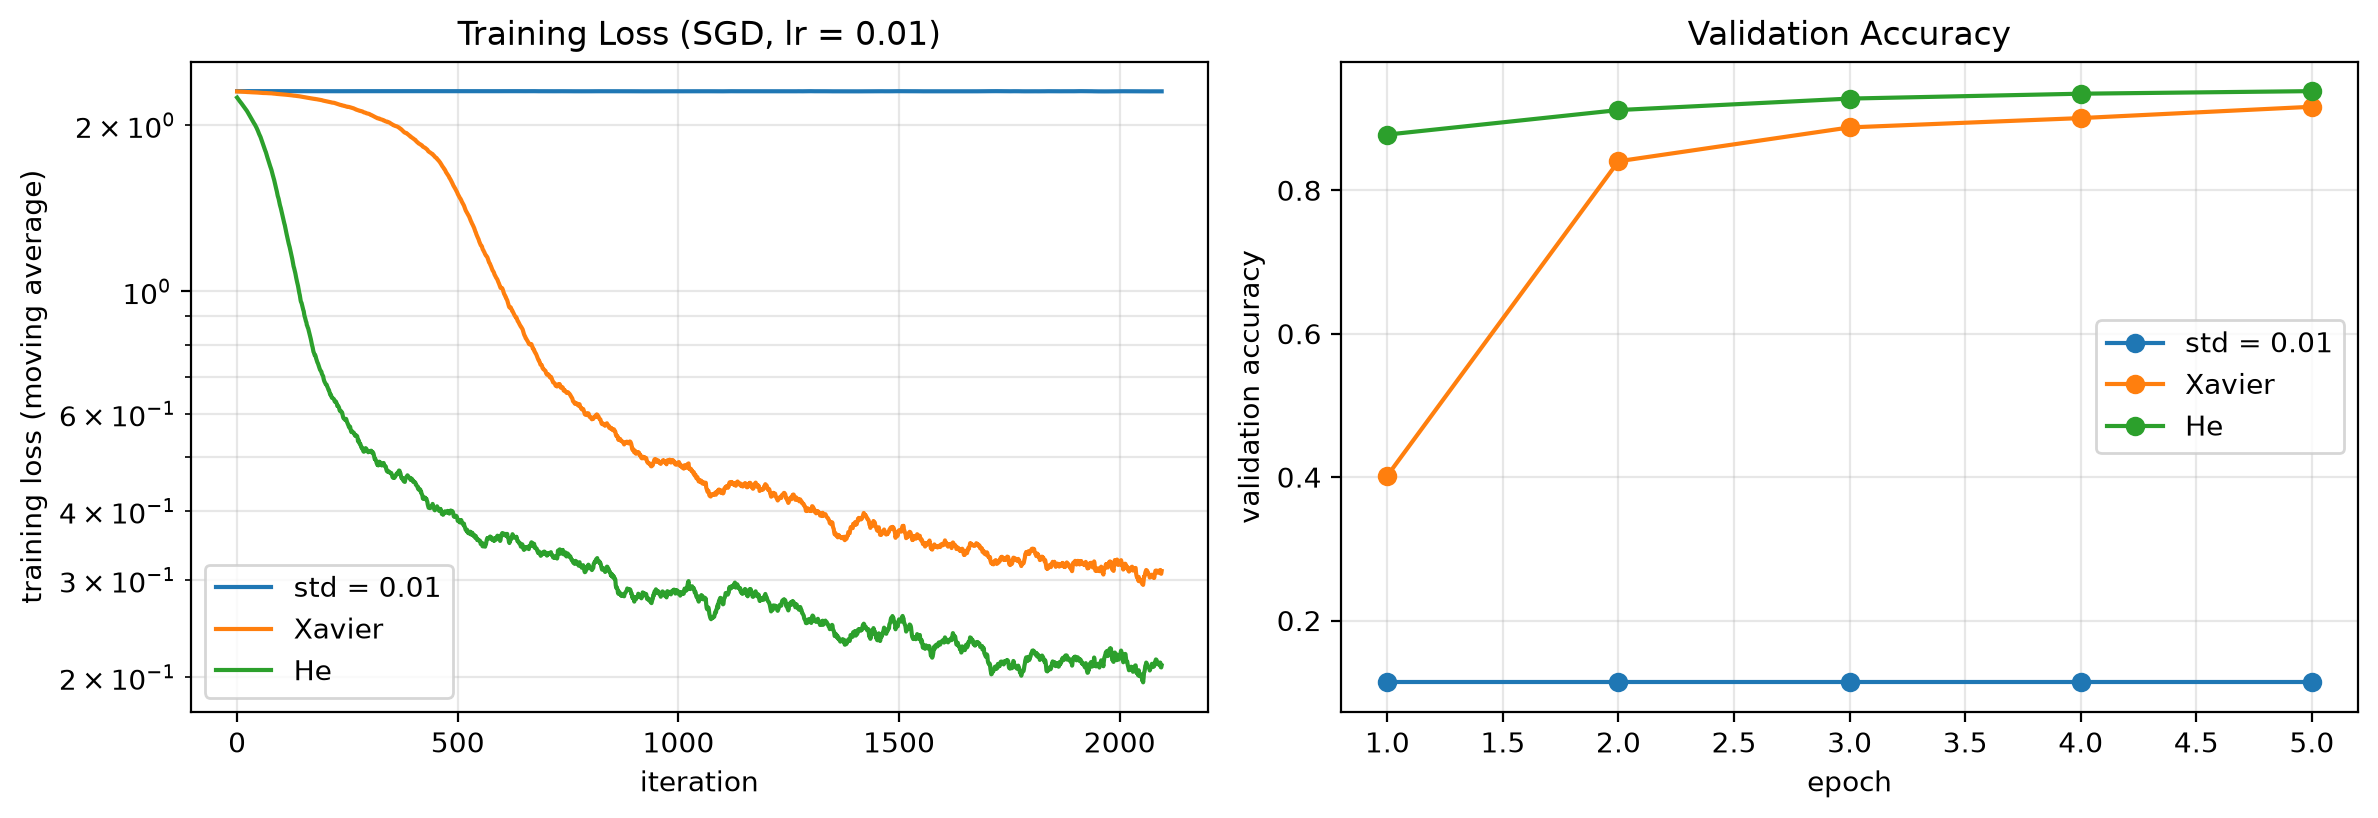
\includegraphics[width=\textwidth]{figures/mnist_init.png}

\small 초깃값에 따른 훈련 손실 (50 iteration 이동평균, 로그 눈금, 왼쪽)과 epoch별 검증 정확도 (오른쪽)
\end{center}
}{%
\begin{center}
\fbox{\parbox{0.8\textwidth}{\centering\small
[그림 자리] \texttt{figures/mnist\_init.png}\\
\texttt{mnist\_init\_compare.py}를 실행하면 생성된다.}}
\end{center}
}

\begin{center}
\begin{tabular}{@{}lccccc@{}}
\toprule
& \multicolumn{5}{c}{검증 정확도} \\
\cmidrule(l){2-6}
초깃값 & 1 epoch & 2 epoch & 3 epoch & 4 epoch & 5 epoch \\
\midrule
표준편차 $0.01$ & $11.4\%$ & $11.4\%$ & $11.4\%$ & $11.4\%$ & $11.4\%$ \\
Xavier & $40.2\%$ & $84.0\%$ & $88.8\%$ & $90.1\%$ & $91.6\%$ \\
He & $87.8\%$ & $91.2\%$ & $92.8\%$ & $93.5\%$ & $93.8\%$ \\
\bottomrule
\end{tabular}
\end{center}

\begin{itemize}[leftmargin=1.8em]
\item \textbf{표준편차 $0.01$}: 손실이 $\log10\approx2.30$에서 전혀 줄지 않는다.
앞의 실험에서 본 것처럼 신호가 층을 지나며 사라져 gradient도 거의 $0$이기 때문이다.
\item \textbf{Xavier}: 학습은 되지만 처음 $500$ iteration 정도는 느리다.
\item \textbf{He}: 처음부터 빠르게 학습한다. ReLU에 맞춘 초깃값이기 때문이다.
\end{itemize}
optimizer는 똑같이 SGD인데도, 초깃값만 바꾸어 학습이 전혀 되지 않던 network가 잘 학습된다.
\ref{sec:mnistopt}절에서 SGD가 느렸던 것도 optimizer보다 \textbf{초깃값의 문제}였음을 알 수 있다.

\begin{remarkbox}[실무에서의 초기화]
\begin{itemize}[leftmargin=1.5em]
\item Xavier와 He는 지금도 가장 기본이 되는 초기화이다.
CNN과 MLP에서는 ReLU면 He, tanh나 sigmoid면 Xavier를 쓰는 것이 표준이다.
\item PyTorch의 \texttt{nn.Linear}, \texttt{nn.Conv2d}는 따로 지정하지 않아도 He(Kaiming) 계열의 균등분포로 초기화된다
(분산이 $\frac{1}{3n}$이 되도록 조정된 값).
직접 지정할 때는 \texttt{torch.nn.init.xavier\_normal\_}, \texttt{torch.nn.init.kaiming\_normal\_} 등을 쓴다.
\item Transformer와 대규모 언어모델에서는 작은 고정 표준편차(예: $0.02$)의 정규분포를 흔히 쓰고,
층이 깊을수록 잔차(residual) 경로의 출력층을 더 작게 초기화하는 방법을 함께 쓴다.
\item 이 밖에 RNN에서의 직교(orthogonal) 초기화, 잔차 블록의 마지막 층을 $0$으로 초기화하는 방법 등이 있다.
\item 다음에 다룰 \textbf{배치 정규화}는 각 층의 활성화값 분포를 학습 중에 직접 맞추어 주므로,
초깃값에 대한 민감도를 크게 줄여 준다.
\end{itemize}
\end{remarkbox}

% =================================================
\section{배치 정규화}\label{sec:bn}
% =================================================

\ref{sec:init}절에서는 각 층의 활성화값이 적당히 퍼진 분포를 가져야 학습이 잘 된다는 것을 보았고,
그런 분포가 나오도록 \textbf{초깃값}을 고르는 방법(Xavier, He)을 배웠다.
그런데 초깃값으로 맞춘 분포는 학습이 시작되어 가중치가 바뀌면 다시 흐트러진다.
그렇다면 아예 \textbf{각 층에서 활성화값의 분포를 강제로 맞추어 주면} 어떨까?
이것이 \textbf{배치 정규화(Batch Normalization)}의 아이디어이다
(Ioffe \& Szegedy, 2015).

\begin{keybox}[배치 정규화의 장점]
\begin{itemize}[leftmargin=1.5em]
\item 학습을 빨리 진행할 수 있다 (더 큰 학습률을 쓸 수 있다).
\item 초깃값에 크게 의존하지 않는다.
\item overfitting을 억제한다 (dropout 등의 필요성이 줄어든다).
\end{itemize}
\end{keybox}

\subsection{배치 정규화 계층을 넣은 신경망}\label{sec:bnnet}

배치 정규화는 \textbf{하나의 계층(BatchNorm 계층)}으로 구현하여 신경망에 끼워 넣는다.
보통 Affine 계층과 활성화 함수 계층 사이에 넣는다.

\begin{center}
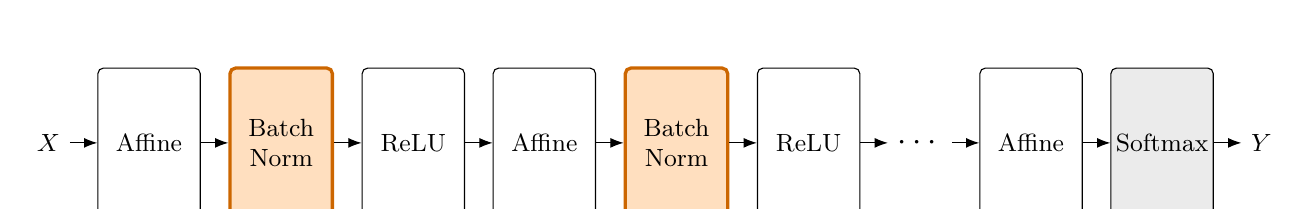
\begin{tikzpicture}[>=Latex,
  lay/.style={draw,rounded corners=2pt,minimum width=13mm,minimum height=19mm,
              font=\small,align=center,inner sep=1pt},
  bn/.style={lay,fill=orange!25,draw=orange!80!black,very thick},
  node distance=3.5mm]
\node[font=\small] (in) {$X$};
\node[lay,right=of in] (a1) {Affine};
\node[bn,right=of a1] (b1) {Batch\\Norm};
\node[lay,right=of b1] (r1) {ReLU};
\node[lay,right=of r1] (a2) {Affine};
\node[bn,right=of a2] (b2) {Batch\\Norm};
\node[lay,right=of b2] (r2) {ReLU};
\node[font=\large,right=of r2] (dots) {$\cdots$};
\node[lay,right=of dots] (a3) {Affine};
\node[lay,right=of a3,fill=black!8] (sm) {Softmax};
\node[font=\small,right=of sm] (out) {$Y$};
\foreach \u/\v in {in/a1,a1/b1,b1/r1,r1/a2,a2/b2,b2/r2,r2/dots,dots/a3,a3/sm,sm/out}
  \draw[->] (\u) -- (\v);
\end{tikzpicture}

\small 배치 정규화를 사용한 신경망의 예 (주황색이 BatchNorm 계층).
마지막 Affine 계층 뒤에는 넣지 않는다.
\end{center}

\subsection{배치 정규화의 순전파}\label{sec:bnforward}

미니배치의 크기를 $h$, 어떤 층의 node 수를 $m$이라 하자.
Affine 계층의 출력 $X$는 $h\times m$ 행렬이고, $i$번째 행은 $i$번째 데이터, $j$번째 열은 $j$번째 node이다.
배치 정규화는 \textbf{node(열)마다 따로}, 미니배치에 들어 있는 $h$개의 데이터에 대하여 평균이 $0$, 분산이 $1$이 되도록 정규화한다.

\begin{center}
\begin{tikzpicture}[x=6mm,y=5mm]
\foreach \i in {0,...,5}{\foreach \j in {0,...,6}{
  \draw[black!40] (\j,-\i) rectangle (\j+1,-\i-1);}}
\fill[orange!25] (3,0) rectangle (4,-6);
\draw[orange!80!black,very thick] (3,0) rectangle (4,-6);
\draw[thick] (0,0) rectangle (7,-6);
\node[above] at (3.5,0.1) {\small $j$번째 열};
\draw[decorate,decoration={brace,amplitude=4pt}] (-0.3,-6) -- (-0.3,0)
  node[midway,left=5pt,font=\small] {$h$개 데이터};
\draw[decorate,decoration={brace,amplitude=4pt,mirror}] (0,-6.3) -- (7,-6.3)
  node[midway,below=5pt,font=\small] {$m$개 node};
\node[right,font=\small,align=left] at (8,-3)
  {$x_{1j},\,x_{2j},\,\ldots,\,x_{hj}$의\\ 평균 $\mu_j$, 분산 $\sigma_j^2$를 구한다\\[2pt]
   $\Rightarrow$ \texttt{np.mean(X, axis=0)}};
\end{tikzpicture}
\end{center}

$j$번째 node에 대하여 (첨자 $j$는 생략한다)
\begin{align}
\mu_B &= \frac1h\sum_{i=1}^{h}x_i
&& \text{(미니배치 평균)}\label{eq:bnmu}\\
\sigma_B^2 &= \frac1h\sum_{i=1}^{h}(x_i-\mu_B)^2
&& \text{(미니배치 분산)}\label{eq:bnvar}\\
\hat x_i &= \frac{x_i-\mu_B}{\sqrt{\sigma_B^2+\varepsilon}}
&& \text{(정규화)}\label{eq:bnhat}\\
y_i &= \gamma\,\hat x_i+\beta
&& \text{(확대 $\gamma$와 이동 $\beta$)}\label{eq:bny}
\end{align}
이다. $\varepsilon$은 $0$으로 나누는 것을 막는 작은 수 ($10^{-7}$)이다.

\begin{itemize}[leftmargin=1.8em]
\item \eqref{eq:bnmu}--\eqref{eq:bnhat}을 거치면 각 node의 값 $\hat x_1,\ldots,\hat x_h$는
평균 $0$, 분산 (거의) $1$이 된다.
\item 그런데 모든 층의 입력을 평균 $0$, 분산 $1$로 고정하면 network의 표현력이 제한될 수 있다.
예를 들어 sigmoid의 입력이 항상 $0$ 근처에만 있으면 sigmoid는 거의 직선처럼 동작한다.
그래서 \eqref{eq:bny}에서 \textbf{학습되는 parameter} $\gamma$(scale)와 $\beta$(shift)로 분포를 다시 조정할 수 있게 한다.
$\gamma=1$, $\beta=0$에서 시작하고, $W$, $B$와 똑같이 gradient로 갱신한다.
\item $\gamma=\sqrt{\sigma_B^2+\varepsilon}$, $\beta=\mu_B$로 학습되면 원래의 $x_i$로 되돌아갈 수도 있다.
즉, 정규화가 필요 없으면 network가 스스로 정규화를 ``취소''할 수 있다.
\end{itemize}

행렬로 쓰면, $X$가 $h\times m$일 때 $\bm\mu_B,\ \bm\sigma_B^2,\ \bm\gamma,\ \bm\beta$는 모두 $1\times m$이고
\[
\hat X=\frac{X-\bm\mu_B}{\sqrt{\bm\sigma_B^2+\varepsilon}},\qquad
Y=\bm\gamma\odot\hat X+\bm\beta
\]
이다. $1\times m$ 행벡터가 $h$개의 행에 broadcast된다는 점은 Affine 계층의 $B$와 같다.

\begin{thinkbox}[Affine 계층의 bias $B$는 필요 없다]
BatchNorm 바로 앞의 Affine 계층의 출력은 $X=X_{\text{in}}W+B$이다.
$B$는 모든 행에 같은 값을 더하므로 평균 $\bm\mu_B$도 정확히 $B$만큼 커지고,
$X-\bm\mu_B$에서 $B$는 사라진다.
즉 BatchNorm 앞의 $B$는 출력에 아무 영향이 없고, 그 역할은 $\bm\beta$가 대신한다.
실제로 아래의 gradient 확인에서 $\pd{L}{B_1}$은 $0$이다.
그래서 PyTorch에서는 보통 \texttt{nn.Linear(n\_in, n\_out, bias=False)} 다음에 \texttt{nn.BatchNorm1d(n\_out)}를 둔다.
이 강의의 코드에서는 구조를 단순하게 하려고 $B$를 그대로 두었다.
\end{thinkbox}

\subsection{배치 정규화의 계산 그래프와 역전파}\label{sec:bngraph}

순전파 \eqref{eq:bnmu}--\eqref{eq:bny}를 작은 계산으로 나누어 변수 노드 기준의 계산 그래프로 그리면 다음과 같다.
중간 변수의 이름은 코드와 같게 하였다.
\[
\bm\mu=\frac1h\sum_{i}X_{i,:},\quad
X_c=X-\bm\mu,\quad
\bm v=\frac1h\sum_{i}(X_c)_{i,:}^2,\quad
\bm s=\sqrt{\bm v+\varepsilon},\quad
\hat X=\frac{X_c}{\bm s},\quad
Y=\bm\gamma\odot\hat X+\bm\beta
\]
($\bm\mu$: \texttt{mu}, $X_c$: \texttt{xc}, $\bm v$: \texttt{var}, $\bm s$: \texttt{std}, $\hat X$: \texttt{xn}).

\begin{center}
\begin{tikzpicture}[>=Latex,
  var/.style={draw,circle,minimum size=13mm,align=center,inner sep=0pt},
  fw/.style={->,thick},
  bl/.style={orange!85!black,font=\normalsize}]
\node[var] (X)  at (0,0)     {$X$\\[-3pt]{\scriptsize $h\times m$}};
\node[var] (mu) at (2.4,2.3) {$\bm\mu$\\[-3pt]{\scriptsize $1\times m$}};
\node[var] (Xc) at (4.8,0)   {$X_c$\\[-3pt]{\scriptsize $h\times m$}};
\node[var] (v)  at (6.6,-2.6){$\bm v$\\[-3pt]{\scriptsize $1\times m$}};
\node[var] (s)  at (9.4,-2.6){$\bm s$\\[-3pt]{\scriptsize $1\times m$}};
\node[var] (Xh) at (11.2,0)  {$\hat X$\\[-3pt]{\scriptsize $h\times m$}};
\node[var] (Y)  at (14.6,0)  {$Y$\\[-3pt]{\scriptsize $h\times m$}};
\draw[fw] (X) -- node[above left,font=\small] {평균} (mu);
\draw[fw] (X) -- node[below,font=\small] {$-$} (Xc);
\draw[fw] (mu) -- node[above right,font=\small] {$-$} (Xc);
\draw[fw] (Xc) -- node[left,font=\small] {제곱의 평균} (v);
\draw[fw] (v) -- node[below,font=\small] {$\sqrt{\,\cdot+\varepsilon}$} (s);
\draw[fw] (Xc) -- node[below,font=\small] {$\div$} (Xh);
\draw[fw] (s) -- node[right,font=\small] {$\div$} (Xh);
\draw[fw] (Xh) -- node[above,font=\small] {$\bm\gamma,\ \bm\beta$} (Y);
% gradients (orange)
\node[bl,anchor=south] at (Y.north) {\ding{172}\ $\pd{L}{Y}$};
\node[bl,anchor=south] at (Xh.north) {\ding{173}\ $\pd{L}{\hat X}$};
\node[bl,anchor=north] at (s.south) {\ding{174}\ $\pd{L}{\bm s}$};
\node[bl,anchor=north] at (v.south) {\ding{175}\ $\pd{L}{\bm v}$};
\node[bl,anchor=south] at ([yshift=1mm]Xc.north) {\ding{176}\ $\pd{L}{X_c}$};
\node[bl,anchor=south] at (mu.north) {\ding{177}\ $\pd{L}{\bm\mu}$};
\node[bl,anchor=north] at ([yshift=-1mm]X.south) {\ding{178}\ $\pd{L}{X}$};
\end{tikzpicture}

\small 배치 정규화의 계산 그래프 (변수 노드 기준).
검은 화살표가 순전파, 주황색 번호는 역전파에서 gradient를 구하는 순서이다.
\end{center}

역전파는 오른쪽에서 왼쪽으로, \ding{172}부터 \ding{178}까지 차례로 gradient를 구한다.
지금까지의 계산 그래프와 다른 점은 \textbf{한 변수에서 화살표가 두 개 이상 나가는 경우}가 있다는 것이다
($X\to\bm\mu,\ X\to X_c$와 $X_c\to\bm v,\ X_c\to\hat X$).
이때 그 변수의 gradient는 \textbf{각 경로로 돌아오는 gradient의 합}이다 (다변수 연쇄법칙).
또 $1\times m$인 변수($\bm\mu$, $\bm v$, $\bm s$, $\bm\gamma$, $\bm\beta$)는 순전파에서 $h$개의 행에 broadcast되었으므로,
역전파에서는 Affine 계층의 $B$와 마찬가지로 \textbf{행 방향으로 합한다} (\texttt{np.sum(..., axis=0)}).

\begin{itemize}[leftmargin=2.2em,itemsep=0.5em]
\item[\ding{173}] $Y=\bm\gamma\odot\hat X+\bm\beta$:
\[
\pd{L}{\bm\beta}=\sum_{i}\Bigl(\pd{L}{Y}\Bigr)_{i,:},\qquad
\pd{L}{\bm\gamma}=\sum_{i}\Bigl(\hat X\odot\pd{L}{Y}\Bigr)_{i,:},\qquad
\pd{L}{\hat X}=\bm\gamma\odot\pd{L}{Y}.
\]
\item[\ding{174}] $\hat X=X_c/\bm s$에서 $\bm s$로 가는 경로:
\[
\pd{L}{\bm s}=-\sum_i\Bigl(\pd{L}{\hat X}\odot\frac{X_c}{\bm s^2}\Bigr)_{i,:}.
\]
\item[\ding{175}] $\bm s=\sqrt{\bm v+\varepsilon}$:
\[
\pd{L}{\bm v}=\pd{L}{\bm s}\cdot\frac{1}{2\sqrt{\bm v+\varepsilon}}=\frac{1}{2\bm s}\pd{L}{\bm s}.
\]
\item[\ding{176}] $X_c$는 $\hat X$와 $\bm v$ 두 곳으로 가므로 두 gradient를 더한다.
$\bm v=\frac1h\sum_i (X_c)_{i,:}^2$에서 $\pd{\bm v}{(X_c)_{i,:}}=\frac2h(X_c)_{i,:}$이므로
\[
\pd{L}{X_c}=\underbrace{\frac{1}{\bm s}\odot\pd{L}{\hat X}}_{\hat X\text{ 경로}}
+\underbrace{\frac2h\,X_c\odot\pd{L}{\bm v}}_{\bm v\text{ 경로}}.
\]
\item[\ding{177}] $X_c=X-\bm\mu$에서 $\bm\mu$ (broadcast되었으므로 합한다):
\[
\pd{L}{\bm\mu}=-\sum_i\Bigl(\pd{L}{X_c}\Bigr)_{i,:}.
\]
\item[\ding{178}] $X$는 $X_c$와 $\bm\mu$ 두 곳으로 간다. $\bm\mu=\frac1h\sum_iX_{i,:}$에서 $\pd{\bm\mu}{X_{i,:}}=\frac1h$이므로
\[
\pd{L}{X}=\pd{L}{X_c}+\frac1h\pd{L}{\bm\mu}
=\pd{L}{X_c}-\frac1h\sum_i\Bigl(\pd{L}{X_c}\Bigr)_{i,:}.
\]
\end{itemize}
\ding{173}에서는 $\pd{L}{\hat X}$와 함께 parameter의 gradient $\pd{L}{\bm\beta}$, $\pd{L}{\bm\gamma}$도 구한다.

\begin{remarkbox}[한 줄로 정리한 $\pd{L}{X}$]
위의 단계를 모두 대입하면 (node 하나에 대하여, $g_i=\pd{L}{\hat x_i}$)
\[
\pd{L}{x_i}=\frac{1}{\sqrt{\sigma_B^2+\varepsilon}}
\Bigl(g_i-\frac1h\sum_{k=1}^{h}g_k-\hat x_i\cdot\frac1h\sum_{k=1}^{h}g_k\hat x_k\Bigr)
\]
이다. $g_i$에서 \textbf{평균 방향 성분}과 \textbf{$\hat x$ 방향 성분}을 빼고 $\sigma_B$로 나눈 것이다.
따라서 $\sum_i\pd{L}{x_i}=0$이다. 입력에 같은 상수를 더해도 정규화된 결과는 그대로이므로,
그 방향으로는 gradient가 없는 것이 당연하다. (BatchNorm 앞의 bias $B$의 gradient가 $0$인 이유이기도 하다.)
\end{remarkbox}

\subsection{학습할 때와 추론할 때}\label{sec:bntest}

학습할 때는 미니배치의 평균과 분산으로 정규화한다.
그런데 학습이 끝난 network로 \textbf{데이터 하나}를 분류할 때는 미니배치 평균을 구할 수 없고,
같은 데이터가 어떤 미니배치에 들어 있느냐에 따라 출력이 달라져서도 안 된다.
그래서 학습하는 동안 미니배치 평균과 분산의 \textbf{지수이동평균}을 기억해 두었다가
\[
\bm\mu_{\text{run}}\leftarrow0.9\,\bm\mu_{\text{run}}+0.1\,\bm\mu_B,\qquad
\bm\sigma^2_{\text{run}}\leftarrow0.9\,\bm\sigma^2_{\text{run}}+0.1\,\bm\sigma^2_B,
\]
추론(검증, 시험)할 때는 이 값으로 정규화한다.
\[
\hat X=\frac{X-\bm\mu_{\text{run}}}{\sqrt{\bm\sigma^2_{\text{run}}+\varepsilon}},\qquad Y=\bm\gamma\odot\hat X+\bm\beta.
\]
이 지수이동평균은 Momentum과 Adam의 $m$, $v$와 같은 방식이다 (\ref{sec:momentum}, \ref{sec:adam}절).
그래서 BatchNorm 계층의 \texttt{forward}는 학습 중인지를 알려 주는 \texttt{train\_flg}를 받는다.
PyTorch에서 \texttt{model.train()}과 \texttt{model.eval()}을 구분해야 하는 가장 큰 이유가 이것이다.

\subsection{BatchNorm 계층의 구현}\label{sec:bncode}

\texttt{layers.py}에 \texttt{BatchNormalization} 계층을 추가하였다.
\texttt{backward}의 각 줄이 위의 \ding{172}--\ding{178}에 그대로 대응한다.
\begin{lstlisting}
class BatchNormalization:
    """Normalize each node (column) over the mini-batch, then scale and shift:
       x_hat = (x - mu) / sqrt(var + eps),   y = gamma * x_hat + beta"""
    def __init__(self, gamma, beta, momentum=0.9, eps=1e-7):
        self.gamma = gamma          # (1, m)
        self.beta = beta            # (1, m)
        self.momentum = momentum
        self.eps = eps
        self.running_mean = None    # used at test time
        self.running_var = None
        self.dgamma = None
        self.dbeta = None

    def forward(self, X, train_flg=True):
        if self.running_mean is None:
            self.running_mean = np.zeros((1, X.shape[1]))
            self.running_var = np.ones((1, X.shape[1]))
        if train_flg:                                     # statistics of THIS mini-batch
            mu = np.mean(X, axis=0, keepdims=True)        # (1, m)
            xc = X - mu                                   # (h, m)
            var = np.mean(xc ** 2, axis=0, keepdims=True) # (1, m)
            std = np.sqrt(var + self.eps)
            xn = xc / std                                 # x_hat (h, m)
            self.h, self.xc, self.std, self.xn = X.shape[0], xc, std, xn
            self.running_mean = self.momentum * self.running_mean + (1 - self.momentum) * mu
            self.running_var = self.momentum * self.running_var + (1 - self.momentum) * var
        else:                                             # test time: running averages
            xn = (X - self.running_mean) / np.sqrt(self.running_var + self.eps)
        return self.gamma * xn + self.beta

    def backward(self, dY):
        self.dbeta = np.sum(dY, axis=0, keepdims=True)              # (1, m)
        self.dgamma = np.sum(self.xn * dY, axis=0, keepdims=True)   # (1, m)
        dxn = self.gamma * dY                                       # (h, m)
        dxc = dxn / self.std
        dstd = -np.sum(dxn * self.xc / (self.std * self.std), axis=0, keepdims=True)
        dvar = 0.5 * dstd / self.std
        dxc += (2.0 / self.h) * self.xc * dvar
        dmu = np.sum(dxc, axis=0, keepdims=True)
        return dxc - dmu / self.h                                   # dL/dX (h, m)
\end{lstlisting}

\begin{center}
\small
\begin{tabular}{@{}cll@{}}
\toprule
단계 & 식 & 코드 \\
\midrule
\ding{173} & $\pd{L}{\bm\beta}$, $\pd{L}{\bm\gamma}$, $\pd{L}{\hat X}$ & \texttt{dbeta}, \texttt{dgamma}, \texttt{dxn} \\
\ding{174} & $\pd{L}{\bm s}$ & \texttt{dstd} \\
\ding{175} & $\pd{L}{\bm v}$ & \texttt{dvar} \\
\ding{176} & $\pd{L}{X_c}$ ($\hat X$ 경로 $+$ $\bm v$ 경로) & \texttt{dxc = dxn / std}, \ \texttt{dxc += ...} \\
\ding{177} & $\pd{L}{\bm\mu}$ (부호를 뺀 값) & \texttt{dmu = np.sum(dxc, ...)} \\
\ding{178} & $\pd{L}{X}=\pd{L}{X_c}-\frac1h\sum_i(\cdot)$ & \texttt{return dxc - dmu / self.h} \\
\bottomrule
\end{tabular}
\end{center}
코드의 \texttt{dmu}는 $\sum_i\bigl(\pd{L}{X_c}\bigr)_{i,:}$, 즉 $-\pd{L}{\bm\mu}$이다.

\texttt{MultiLayerNet}에는 \texttt{use\_batchnorm} 옵션을 추가하였다.
\texttt{True}이면 은닉층마다 Affine $\to$ BatchNorm $\to$ 활성화 함수 순서로 계층을 쌓고,
$\bm\gamma$, $\bm\beta$를 \texttt{params}에 \texttt{gamma1}, \texttt{beta1}, $\ldots$의 이름으로 넣는다.
\texttt{params}에 들어 있으므로 optimizer는 $W$, $B$와 똑같이 $\bm\gamma$, $\bm\beta$도 갱신한다.
\begin{lstlisting}
            if i < len(sizes) - 2:                     # hidden layer
                if use_batchnorm:                      # Affine -> BatchNorm -> activation
                    gamma, beta = np.ones((1, n_out)), np.zeros((1, n_out))
                    self.params[f"gamma{i + 1}"] = gamma
                    self.params[f"beta{i + 1}"] = beta
                    self.layers.append(BatchNormalization(gamma, beta))
                self.layers.append(Relu() if activation == "relu" else Sigmoid())
\end{lstlisting}
순전파는 \texttt{train\_flg}를 BatchNorm 계층 (그리고 \ref{sec:dropout}절의 Dropout 계층)에만 넘긴다.
손실(학습)에서는 미니배치 통계를, 정확도(평가)에서는 이동평균을 쓴다.
\begin{lstlisting}
    def predict(self, X, train_flg=False):    # scores U
        for layer in self.layers:
            if isinstance(layer, (BatchNormalization, Dropout)):   # training and test differ
                X = layer.forward(X, train_flg)
            else:
                X = layer.forward(X)
        return X

    def loss(self, X, T):                     # used for training: batch statistics, dropout
        data_loss = self.last.forward(self.predict(X, train_flg=True), T)
\end{lstlisting}
(\texttt{loss}의 나머지 부분인 가중치 감소는 \ref{sec:weightdecay}절에서 다룬다.)
역전파가 끝나면 각 계층에 저장된 gradient를 모은다.
BatchNorm 계층의 번호는 바로 앞 Affine 계층의 번호를 따른다.
\begin{lstlisting}
        grads, k = {}, 0
        for layer in self.layers:
            if isinstance(layer, Affine):
                k += 1
                grads[f"W{k}"], grads[f"B{k}"] = layer.dW, layer.dB
            elif isinstance(layer, BatchNormalization):
                grads[f"gamma{k}"], grads[f"beta{k}"] = layer.dgamma, layer.dbeta
\end{lstlisting}

\paragraph{gradient 확인.}
계산 그래프로 유도한 역전파가 맞는지, 작은 network에서 수치미분과 비교한다
(\texttt{mnist\_batchnorm.py}의 (1)).
\begin{lstlisting}
np.random.seed(0)
small = MultiLayerNet(4, [5, 5], 3, weight_init_std=1.0, use_batchnorm=True)
X_small = np.random.randn(6, 4)
T_small = np.eye(3)[np.random.randint(0, 3, size=6)]
small.loss(X_small, T_small)
grads = small.backward()
for key in small.params:
    num = numerical_gradient(lambda: small.loss(X_small, T_small), small.params[key])
    print(f"{key:7s}: max |backprop - numerical| = {np.max(np.abs(grads[key] - num)):.2e}")
\end{lstlisting}
\begin{lstlisting}[language={},numbers=none]
W1     : max |backprop - numerical| = 2.48e-11
B1     : max |backprop - numerical| = 2.43e-17
gamma1 : max |backprop - numerical| = 2.48e-11
beta1  : max |backprop - numerical| = 1.64e-11
W2     : max |backprop - numerical| = 2.35e-11
B2     : max |backprop - numerical| = 1.11e-11
gamma2 : max |backprop - numerical| = 1.31e-11
beta2  : max |backprop - numerical| = 1.31e-11
W3     : max |backprop - numerical| = 2.85e-11
B3     : max |backprop - numerical| = 1.41e-11
\end{lstlisting}
모든 parameter에서 오차가 $10^{-11}$ 이하이므로 역전파가 올바르다.
$B_1$, $B_2$는 BatchNorm 바로 앞의 bias이므로 역전파로 구한 gradient가 정확히 $0$이다.
($B_1$의 오차가 특히 작은 것은 수치미분도 정확히 $0$이 나왔기 때문이다.)

\subsection{배치 정규화의 효과}\label{sec:bneffect}

\paragraph{실험 1: 가중치의 초깃값을 바꾸어 가며 (책의 실험).}
MNIST의 훈련 데이터 $1000$장만으로, 은닉층 $5$개 (각 $100$개 node, ReLU)인 network를
SGD (학습률 $0.01$, 미니배치 $100$)로 $20$ epoch 학습시킨다.
가중치의 표준편차를 $1$부터 $0.0001$까지 $16$가지로 바꾸어 가며,
\textbf{같은 초깃값, 같은 미니배치}로 배치 정규화가 있을 때와 없을 때를 비교한다.
\begin{lstlisting}
x_small, t_small = x_train[:1000], t_train[:1000]
hidden = [100, 100, 100, 100, 100]               # 5 hidden layers, 100 nodes each
weight_scales = np.logspace(0, -4, num=16)       # 1, ..., 0.0001
epochs_small = 20

fig, axes = plt.subplots(4, 4, figsize=(13, 10))
t0 = time.time()
for ax, w in zip(axes.ravel(), weight_scales):
    curves = {}
    for use_bn in (True, False):
        np.random.seed(1)                         # the SAME initial weights
        net = MultiLayerNet(784, hidden, 10, weight_init_std=w, use_batchnorm=use_bn)
        _, accs = train(net, x_small, t_small, epochs_small, 100, 0.01, x_small, t_small)
        curves[use_bn] = accs
\end{lstlisting}
\texttt{train}은 SGD로 학습하며 epoch마다 정확도를 기록하는 함수이다 (코드 파일 참고).

\IfFileExists{figures/bn_weight_scales.png}{%
\begin{center}
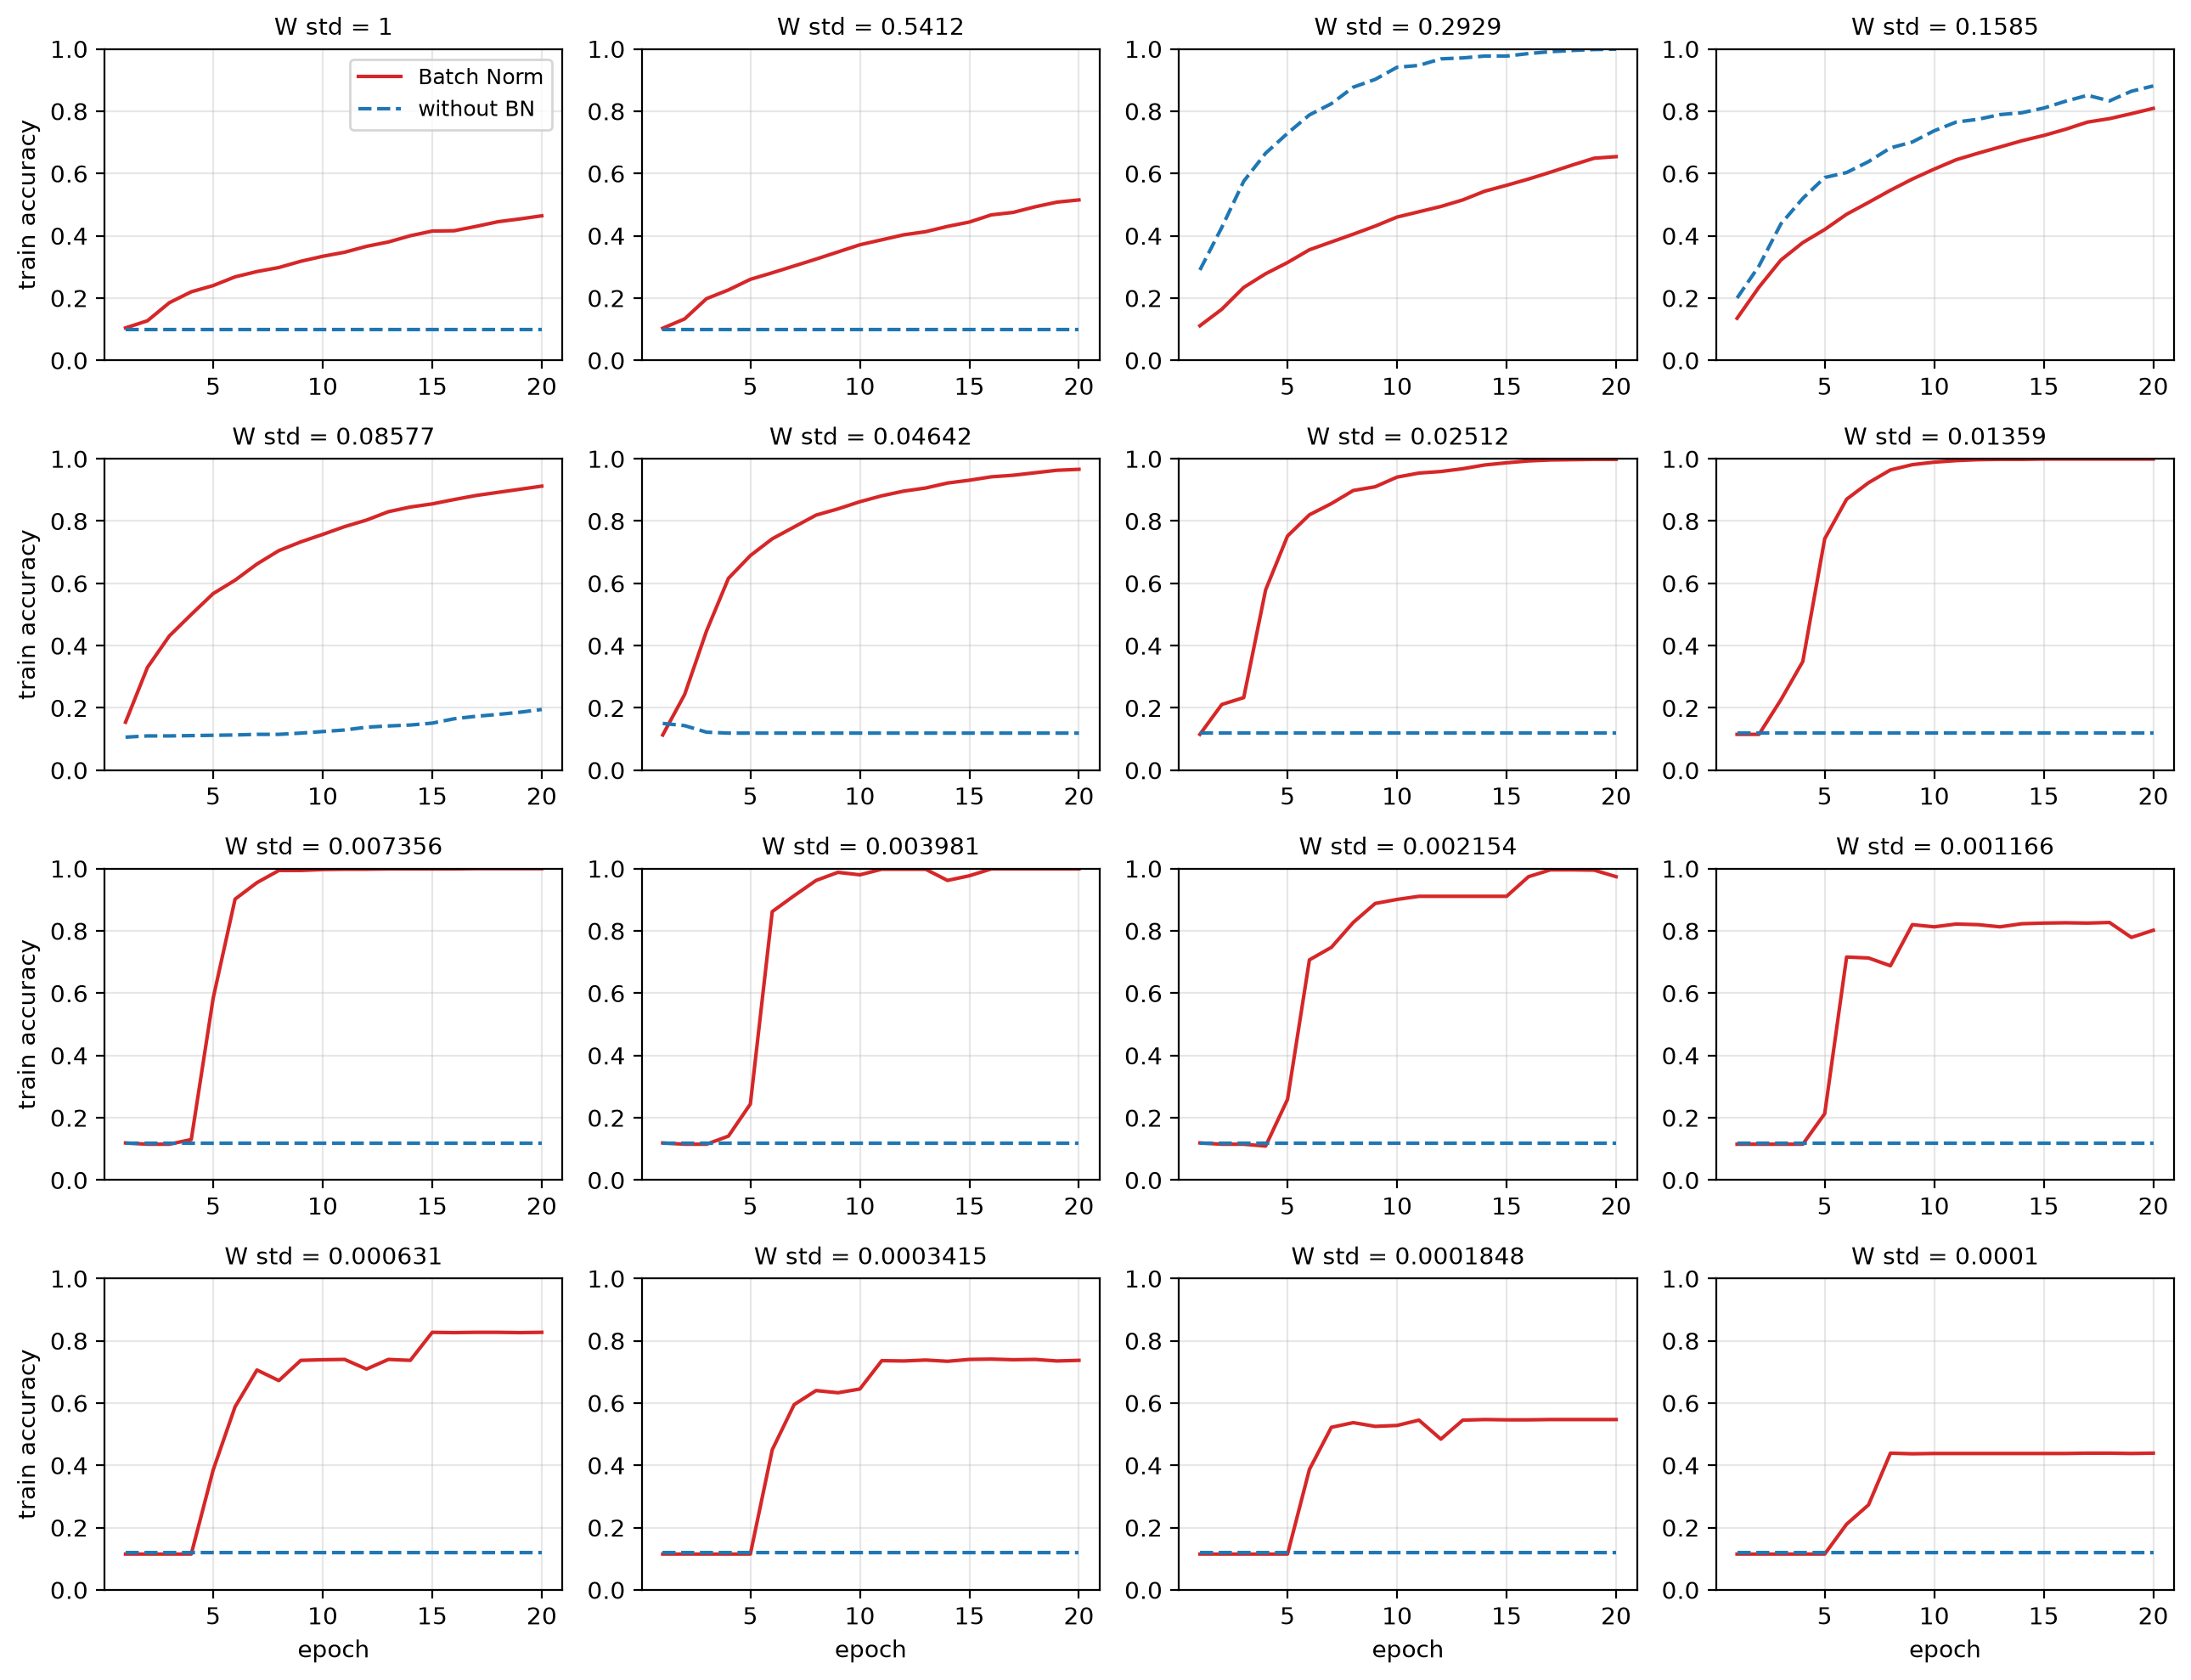
\includegraphics[width=\textwidth]{figures/bn_weight_scales.png}

\small 가중치 초깃값의 표준편차별 훈련 정확도. 실선: 배치 정규화 사용, 점선: 사용하지 않음
\end{center}
}{%
\begin{center}
\fbox{\parbox{0.8\textwidth}{\centering\small
[그림 자리] \texttt{figures/bn\_weight\_scales.png}\\
\texttt{mnist\_batchnorm.py}를 실행하면 생성된다.}}
\end{center}
}

\begin{center}
\small
\begin{tabular}{@{}lcccccccc@{}}
\toprule
가중치 표준편차 & $1$ & $0.29$ & $0.16$ & $0.086$ & $0.025$ & $0.0074$ & $0.0012$ & $0.0001$ \\
\midrule
배치 정규화 사용 & $0.46$ & $0.65$ & $0.81$ & $0.91$ & $\mathbf{1.00}$ & $\mathbf{1.00}$ & $0.80$ & $0.44$ \\
사용하지 않음 & $0.10$ & $\mathbf{1.00}$ & $0.88$ & $0.20$ & $0.12$ & $0.12$ & $0.12$ & $0.12$ \\
\bottomrule
\end{tabular}

$20$ epoch 후의 훈련 정확도 (16가지 중 일부)
\end{center}

\begin{itemize}[leftmargin=1.8em]
\item \textbf{배치 정규화가 없으면} 표준편차가 $0.29$, $0.16$ 근처일 때만 학습이 되고,
그보다 작으면 (\ref{sec:init}절에서 본 것처럼 신호가 사라져) 정확도가 $0.12$ 근처에 머문다.
표준편차가 $1$이면 활성화값이 폭발하여 역시 학습이 되지 않는다.
학습이 되는 초깃값의 범위가 매우 좁다.
\item \textbf{배치 정규화를 쓰면} 거의 모든 초깃값에서 학습이 진행되고,
표준편차 $0.05\sim0.002$에서는 $20$ epoch 안에 훈련 정확도 $96\sim100\%$에 도달한다.
초깃값에 대한 의존성이 크게 줄었다.
\item 표준편차 $0.29$, $0.16$처럼 원래 잘 되는 초깃값에서는 배치 정규화가 오히려 느릴 수도 있다.
배치 정규화가 항상 모든 경우에 더 좋은 것은 아니다.
\end{itemize}

\begin{thinkbox}[왜 초깃값이 너무 크거나 작으면 배치 정규화를 써도 느릴까?]
BatchNorm 앞의 가중치를 $W\to aW$로 $a$배 하면 $X$와 $\bm\mu_B$, $\bm\sigma_B$도 모두 $a$배가 되므로
정규화된 $\hat X$는 \textbf{변하지 않는다}. 즉 손실은 $W$의 크기와 무관하다.
반면 $\pd{L}{(aW)}=\frac1a\pd{L}{W}$이므로 gradient는 $\frac1a$배가 되고,
갱신량을 $W$의 크기에 대한 비율로 보면 $\frac{1}{a^2}$배가 된다.
\begin{itemize}[leftmargin=1.5em]
\item 가중치가 크면 ($a\gg1$) 상대적인 갱신량이 작아서 학습이 \textbf{느리다}
(표준편차 $1$, $0.54$).
\item 가중치가 아주 작으면 ($a\ll1$) 상대적인 갱신량이 매우 커서 학습이 \textbf{불안정}하다.
처음 몇 epoch 동안 정체하다가 갑자기 뛰어오르고, 정확도가 중간에서 멈추기도 한다
(표준편차 $0.001$ 이하).
\end{itemize}
배치 정규화를 쓰면 가중치의 크기가 사실상 \textbf{학습률을 조절하는 역할}을 한다.
그래도 배치 정규화가 없을 때처럼 학습이 완전히 멈추는 경우는 없다.
\end{thinkbox}

\paragraph{실험 2: \ref{sec:mnistopt}절의 network에 배치 정규화를 넣으면.}
\ref{sec:mnistopt}절에서 SGD (학습률 $0.01$)는 은닉층 $4$개 (각 $100$개 node, 표준편차 $0.05$)인 network를
$5$ epoch 동안 거의 학습시키지 못했다 (검증 정확도 $44.0\%$).
같은 network, 같은 초깃값, 같은 SGD에 배치 정규화만 넣어 전체 MNIST로 학습시킨다
(\texttt{mnist\_batchnorm.py}의 (3)).
\begin{lstlisting}
results = {}
for use_bn in (False, True):
    np.random.seed(1)
    net = MultiLayerNet(784, [100, 100, 100, 100], 10, weight_init_std=0.05, use_batchnorm=use_bn)
    results[use_bn] = train(net, x_train, t_train, 5, 128, 0.01, x_val, t_val)
\end{lstlisting}

\IfFileExists{figures/bn_mnist.png}{%
\begin{center}
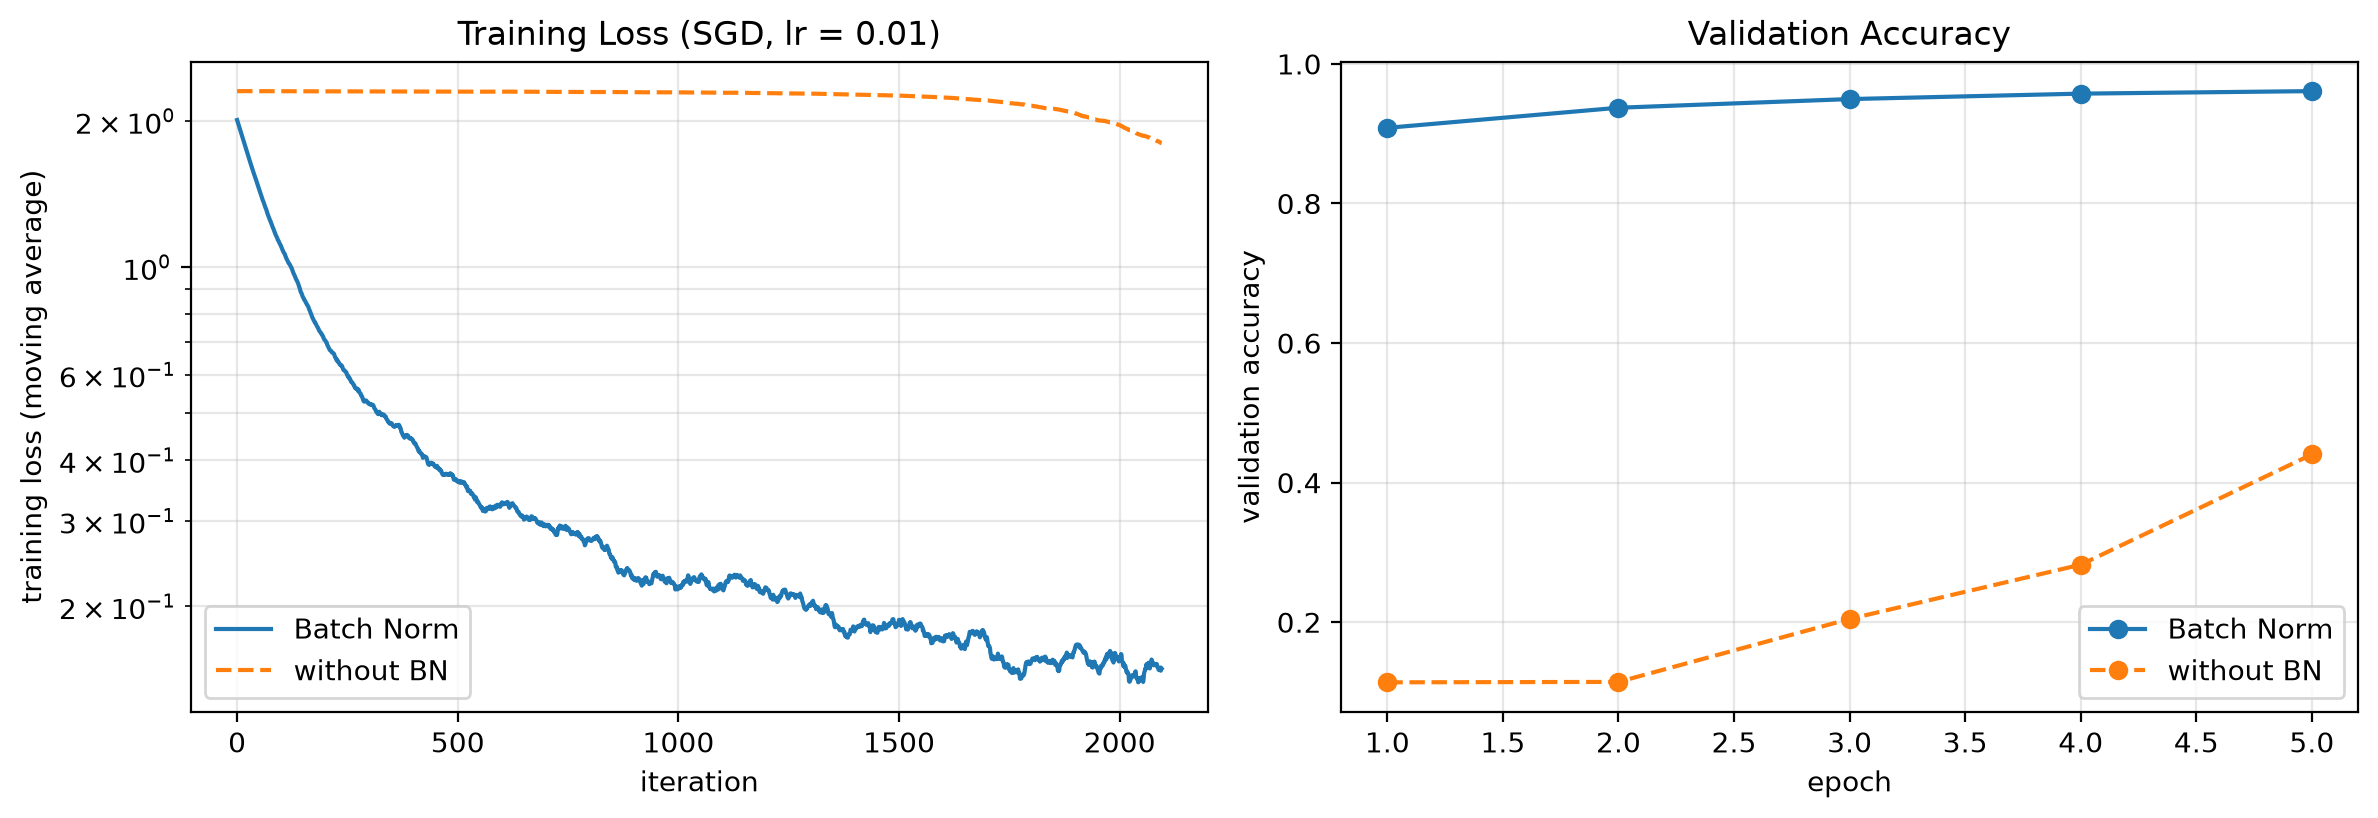
\includegraphics[width=\textwidth]{figures/bn_mnist.png}

\small 배치 정규화 유무에 따른 훈련 손실 (50 iteration 이동평균, 로그 눈금, 왼쪽)과 epoch별 검증 정확도 (오른쪽)
\end{center}
}{%
\begin{center}
\fbox{\parbox{0.8\textwidth}{\centering\small
[그림 자리] \texttt{figures/bn\_mnist.png}\\
\texttt{mnist\_batchnorm.py}를 실행하면 생성된다.}}
\end{center}
}

\begin{center}
\begin{tabular}{@{}lccccc@{}}
\toprule
& \multicolumn{5}{c}{검증 정확도} \\
\cmidrule(l){2-6}
& 1 epoch & 2 epoch & 3 epoch & 4 epoch & 5 epoch \\
\midrule
SGD & $11.4\%$ & $11.4\%$ & $20.5\%$ & $28.2\%$ & $44.0\%$ \\
SGD + 배치 정규화 & $90.8\%$ & $93.7\%$ & $95.0\%$ & $95.7\%$ & $96.1\%$ \\
\bottomrule
\end{tabular}
\end{center}

\begin{itemize}[leftmargin=1.8em]
\item 배치 정규화가 없으면 손실이 $\log10\approx2.30$ 근처의 plateau에서 $1500$ iteration 넘게 벗어나지 못한다.
\item 배치 정규화를 넣으면 \textbf{첫 epoch부터} 검증 정확도가 $90\%$를 넘고,
$5$ epoch 후에는 $96.1\%$로 \ref{sec:mnistopt}절의 Adam ($96.6\%$)에 가깝다.
optimizer는 가장 단순한 SGD 그대로이다.
\item 검증 정확도는 \texttt{train\_flg=False}, 즉 학습 중에 모은 \textbf{이동평균}으로 계산한 것이다.
이동평균으로도 정확도가 높다는 것은 \ref{sec:bntest}절의 추론 방식이 잘 동작한다는 뜻이다.
\end{itemize}

\begin{keybox}[세 가지 해결책의 비교: 같은 문제 / 다른 접근]
\ref{sec:mnistopt}절에서 SGD가 느렸던 network를 세 가지 방법으로 고쳐 보았다.
\begin{itemize}[leftmargin=1.5em]
\item \textbf{optimizer를 바꾼다} (Momentum, AdaGrad, Adam): 작은 gradient도 크게 키워 plateau를 빠져나온다.
\item \textbf{초깃값을 바꾼다} (Xavier, He): 처음부터 신호가 사라지지 않게 한다.
\item \textbf{배치 정규화를 넣는다}: 학습하는 동안 \textbf{계속} 각 층의 분포를 맞춘다.
\end{itemize}
실제로는 세 가지를 \textbf{함께} 쓴다 (예: He 초깃값 $+$ 배치 정규화 $+$ Adam 또는 Momentum SGD).
\end{keybox}

\begin{remarkbox}[배치 정규화는 왜 효과가 있을까? 그리고 그 후]
\begin{itemize}[leftmargin=1.5em]
\item 원래 논문은 앞 층의 가중치가 바뀌면 뒤 층 입력의 분포가 계속 바뀌는 현상
(\textbf{internal covariate shift})을 줄이기 때문이라고 설명하였다.
이후 연구 (Santurkar 등, 2018)에서는 손실 함수의 지형을 \textbf{더 매끄럽게} 만들어
큰 학습률을 쓸 수 있게 하는 효과가 더 중요하다고 보고 있다. 아직 완전히 합의된 설명은 없다.
\item 미니배치마다 평균과 분산이 조금씩 달라지므로 같은 데이터도 매번 약간 다르게 정규화된다.
이 잡음이 \textbf{규제(regularization)} 효과를 낸다.
\item 미니배치가 매우 작으면 ($h=1, 2$) 평균과 분산을 믿을 수 없어 성능이 나빠진다.
그래서 데이터 하나 안에서 정규화하는 \textbf{Layer Normalization}
(Transformer, 대규모 언어모델의 표준), 채널을 묶어 정규화하는 \textbf{Group Normalization} 등이 나왔다.
CNN에서는 지금도 배치 정규화가 기본이다.
\item PyTorch에서는 \texttt{nn.BatchNorm1d} (MLP), \texttt{nn.BatchNorm2d} (CNN), \texttt{nn.LayerNorm}을 쓴다.
PyTorch의 \texttt{momentum=0.1}은 이 노트의 $0.9$와 같은 뜻이다 (새 값의 비율).
\end{itemize}
\end{remarkbox}

% =================================================
\section{바른 학습을 위해: 오버피팅, 가중치 감소, 드롭아웃}\label{sec:reg}
% =================================================

지금까지는 \textbf{훈련 데이터의 손실을 빠르고 안정적으로 줄이는 방법}을 다루었다.
그러나 우리가 정말 원하는 것은 훈련 데이터가 아니라 \textbf{처음 보는 데이터}를 잘 맞히는 network이다.
이 절에서는 훈련 데이터에만 지나치게 맞추어지는 \textbf{오버피팅(overfitting, 과대적합)}과,
이를 억제하는 대표적인 두 방법인 \textbf{가중치 감소(weight decay)}와 \textbf{드롭아웃(dropout)}을 다룬다.
이렇게 오버피팅을 억제하는 기법을 통틀어 \textbf{규제(regularization)}라고 한다.

\subsection{오버피팅}\label{sec:overfit}

오버피팅은 network가 훈련 데이터에만 지나치게 적응하여,
훈련 데이터에 없는 데이터에는 제대로 대응하지 못하는 상태를 말한다.
주로 다음 두 경우에 일어난다.
\begin{itemize}[leftmargin=1.8em]
\item parameter가 많고 표현력이 높은 network
\item 훈련 데이터가 적은 경우
\end{itemize}

\paragraph{실험: 일부러 오버피팅을 일으켜 보자.}
책에서와 같이 MNIST 훈련 데이터 중 \textbf{$300$장만} 사용하고,
은닉층 $6$개 (각 $100$개 node, ReLU, He 초깃값)인 $7$층 network를
SGD (학습률 $0.01$, 미니배치 $100$)로 $300$ epoch 학습시킨다.
parameter는 약 $13$만 개인데 데이터는 $300$개뿐이다.
매 epoch마다 훈련 데이터 $300$장과 시험 데이터 $10000$장의 정확도를 기록한다
(\texttt{mnist\_overfit.py}).
\begin{lstlisting}
x_train, t_train, x_val, t_val, x_test, t_test = load_mnist_split()
x_train, t_train = x_train[:300], t_train[:300]   # only 300 training images -> overfitting

hidden = [100, 100, 100, 100, 100, 100]           # 6 hidden layers (7 Affine layers)
epochs = 300
batch_size = 100
\end{lstlisting}
같은 초깃값, 같은 미니배치로 비교하기 위해 network는 항상 같은 seed로 만든다.
\begin{lstlisting}
def make_net(**options):
    np.random.seed(1)                             # the SAME initial weights
    return MultiLayerNet(784, hidden, 10, weight_init_std="he", **options)
\end{lstlisting}
\begin{lstlisting}
# (1) overfitting
acc = train(make_net(), SGD(lr=0.01))
\end{lstlisting}

\IfFileExists{figures/overfit.png}{%
\begin{center}
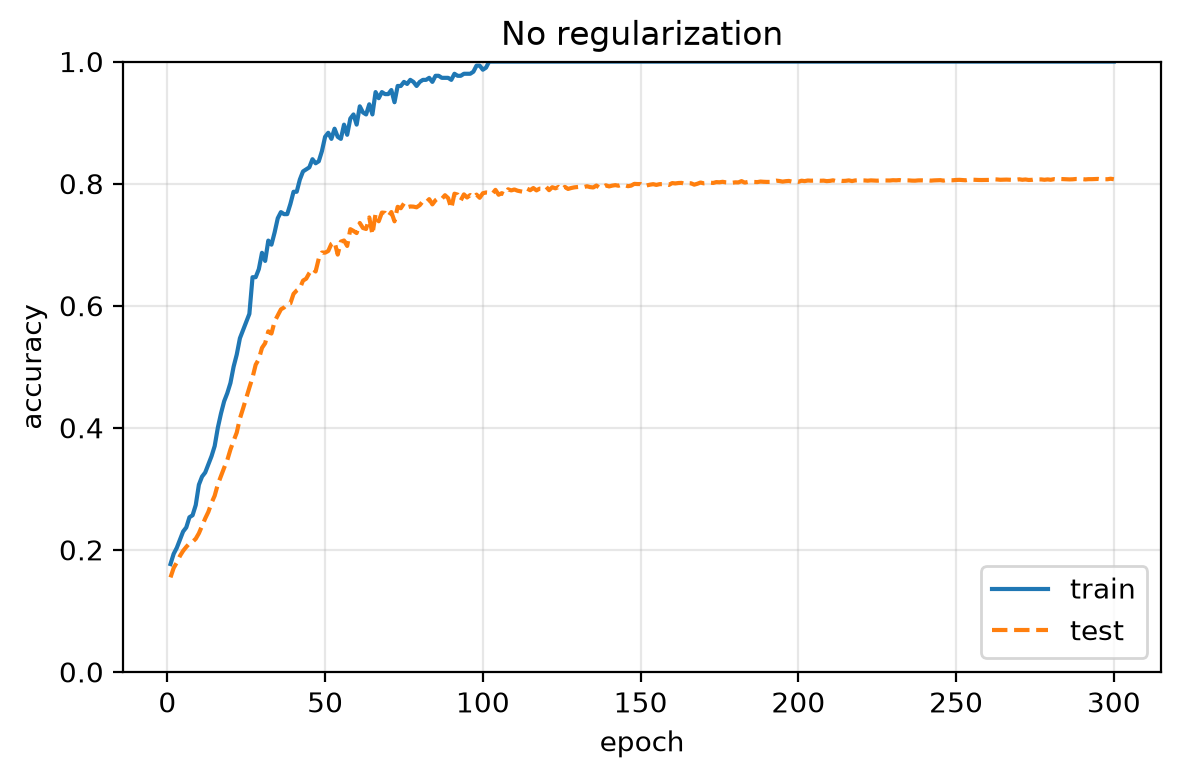
\includegraphics[width=0.62\textwidth]{figures/overfit.png}

\small 규제가 없을 때 훈련 데이터(실선)와 시험 데이터(점선)의 정확도
\end{center}
}{%
\begin{center}
\fbox{\parbox{0.8\textwidth}{\centering\small
[그림 자리] \texttt{figures/overfit.png}\\
\texttt{mnist\_overfit.py}를 실행하면 생성된다.}}
\end{center}
}

약 $100$ epoch 만에 훈련 정확도는 $100\%$가 되지만, 시험 정확도는 $80.7\%$에서 더 오르지 않는다.
이 network는 $300$장의 훈련 데이터를 사실상 \textbf{외워 버린} 것이다.
훈련 정확도가 $100\%$가 된 뒤에는 훈련 데이터에서 더 배울 것이 없으므로 시험 정확도도 그대로이다.
훈련 정확도와 시험 정확도의 차이 ($19.3\%$p)가 오버피팅의 정도를 나타낸다.

\begin{thinkbox}[시험 데이터의 역할]
여기서 시험 데이터는 학습에는 전혀 쓰지 않고, 오버피팅 현상을 보여 주는 데만 썼다.
아래에서 규제의 세기 $\lambda$처럼 사람이 정해야 하는 값을 \textbf{고를} 때는
시험 데이터가 아니라 훈련 데이터에서 떼어 둔 \textbf{검증 데이터}를 쓴다.
그 이유는 \ref{sec:validation}절에서 자세히 다룬다.
\end{thinkbox}

\subsection{가중치 감소}\label{sec:weightdecay}

오버피팅은 가중치 매개변수의 값이 커서 발생하는 경우가 많다.
가중치가 크면 입력이 조금만 달라져도 출력이 크게 바뀌는,
즉 훈련 데이터 하나하나에 날카롭게 맞춘 복잡한 함수가 되기 쉽다.
\textbf{가중치 감소(weight decay)}는 큰 가중치에 벌칙(penalty)을 주어 이를 억제한다.
손실 함수에 모든 가중치의 제곱합(\textbf{L2 norm}의 제곱)을 더한다.
\[
L_{\text{total}}=L+\frac{\lambda}{2}\sum_{k}\lVert W_k\rVert^2,
\qquad \lVert W\rVert^2=\sum_{i,j}w_{ij}^2
\]
$\lambda$는 규제의 세기를 정하는 hyperparameter이다. $\lambda$가 클수록 큰 가중치에 큰 벌칙을 준다.
$\frac12$은 미분을 깔끔하게 하려고 붙인 것이다.

벌칙 항의 미분은 $\pd{}{W}\frac\lambda2\lVert W\rVert^2=\lambda W$이므로,
역전파로 구한 gradient에 $\lambda W$만 더하면 된다.
\[
\pd{L_{\text{total}}}{W}=\pd{L}{W}+\lambda W
\]
이것을 SGD 갱신식에 넣으면
\[
W\leftarrow W-\alpha\Bigl(\pd{L}{W}+\lambda W\Bigr)
=(1-\alpha\lambda)\,W-\alpha\pd{L}{W}
\]
이다. 매 단계마다 가중치를 $(1-\alpha\lambda)$배로 \textbf{줄인(decay)} 뒤 보통의 SGD 갱신을 하는 것과 같다.
그래서 ``가중치 감소''라고 부른다.

\begin{remarkbox}[무엇에 가중치 감소를 적용하는가]
가중치 $W$에만 적용하고, bias $B$와 배치 정규화의 $\bm\gamma$, $\bm\beta$에는 적용하지 않는 것이 보통이다.
bias는 node마다 하나뿐이라 parameter 수가 적고 오버피팅에 거의 기여하지 않으며,
$\bm\gamma$를 $0$ 쪽으로 끌어당기면 오히려 정규화된 신호를 죽이게 되기 때문이다.
코드에서는 이름이 \texttt{"W"}로 시작하는 parameter에만 적용한다.
\end{remarkbox}

\texttt{MultiLayerNet}에 \texttt{weight\_decay\_lambda} 옵션을 추가하였다 (기본값 $0$).
손실에 벌칙 항을 더하고,
\begin{lstlisting}
    def loss(self, X, T):                     # used for training: batch statistics, dropout
        data_loss = self.last.forward(self.predict(X, train_flg=True), T)
        # weight decay: + (lambda/2) * sum of W^2 over all weight matrices (not B, gamma, beta)
        sum_W2 = sum(np.sum(W ** 2) for key, W in self.params.items() if key.startswith("W"))
        return data_loss + 0.5 * self.weight_decay_lambda * sum_W2
\end{lstlisting}
역전파가 끝난 뒤 가중치의 gradient에 $\lambda W$를 더한다.
\begin{lstlisting}
        for key in grads:                     # weight decay: gradient + lambda * W
            if key.startswith("W"):
                grads[key] = grads[key] + self.weight_decay_lambda * self.params[key]
        return grads
\end{lstlisting}
수치미분으로 확인하면 ($\lambda=0.3$) 오차는 $10^{-10}$ 정도로, 벌칙 항의 gradient가 올바르게 구현되었다.

\paragraph{실험.}
앞의 실험과 똑같은 조건에서 $\lambda=0.1$로 가중치 감소를 적용한다.
\begin{lstlisting}
# (2) weight decay
acc = train(make_net(weight_decay_lambda=0.1), SGD(lr=0.01))
\end{lstlisting}

\IfFileExists{figures/overfit_weight_decay.png}{%
\begin{center}
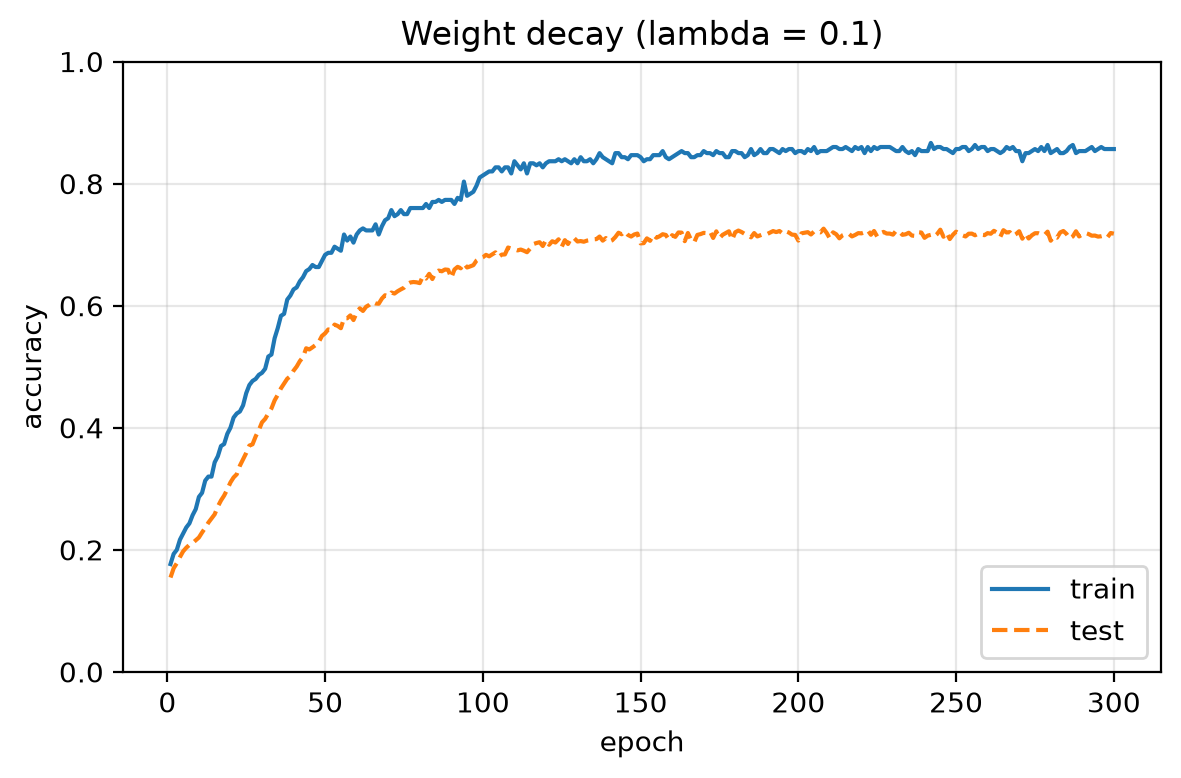
\includegraphics[width=0.62\textwidth]{figures/overfit_weight_decay.png}

\small 가중치 감소 ($\lambda=0.1$)를 적용했을 때의 정확도
\end{center}
}{%
\begin{center}
\fbox{\parbox{0.8\textwidth}{\centering\small
[그림 자리] \texttt{figures/overfit\_weight\_decay.png}\\
\texttt{mnist\_overfit.py}를 실행하면 생성된다.}}
\end{center}
}

훈련 정확도가 $100\%$에 이르지 않고 ($85.7\%$), 훈련과 시험 정확도의 차이가
$19.3\%$p에서 $13.9\%$p로 줄었다. 오버피팅이 억제된 것이다.
다만 이 실험에서는 시험 정확도 자체도 $80.7\%$에서 $71.8\%$로 내려갔다.
$\lambda=0.1$은 이 network에는 \textbf{너무 강한} 규제인 것이다.

\paragraph{$\lambda$는 얼마로 해야 할까?}
$\lambda$를 바꾸어 가며 학습시키고, \textbf{검증 데이터}의 정확도를 비교한다.
\begin{lstlisting}
for lam in (0.0, 0.01, 0.03, 0.1, 0.3):
    net = make_net(weight_decay_lambda=lam)
    train_acc, _ = train(net, SGD(lr=0.01))
    print(f"lambda = {lam:<5}: train {train_acc[-1]:.4f}  validation {net.accuracy(x_val, t_val):.4f}")
\end{lstlisting}

\begin{center}
\begin{tabular}{@{}lccccc@{}}
\toprule
$\lambda$ & $0$ & $0.01$ & $0.03$ & $0.1$ & $0.3$ \\
\midrule
훈련 정확도 & $100\%$ & $100\%$ & $100\%$ & $85.7\%$ & $12.0\%$ \\
검증 정확도 & $80.3\%$ & $80.6\%$ & $\mathbf{80.9\%}$ & $70.8\%$ & $11.4\%$ \\
\bottomrule
\end{tabular}
\end{center}

\begin{itemize}[leftmargin=1.8em]
\item $\lambda$가 너무 크면 ($0.3$) 가중치를 키우지 못하여 훈련 데이터조차 학습하지 못한다.
오버피팅의 반대인 \textbf{과소적합(underfitting)}이다.
\item 적당한 $\lambda$ ($0.03$)에서는 검증 정확도가 조금 오른다.
규제의 세기에는 이처럼 \textbf{적당한 값}이 있고, 그 값은 검증 데이터로 찾는다.
\item 데이터가 $300$장뿐이므로 어떤 규제를 써도 큰 향상은 어렵다.
오버피팅의 가장 확실한 해결책은 \textbf{데이터를 늘리는 것}이다
(전체 $55000$장으로 학습한 \ref{sec:bneffect}절의 network는 검증 정확도가 $96\%$였다).
\end{itemize}

\subsection{Adam과 가중치 감소: AdamW}\label{sec:adamw}

SGD에서는 ``손실에 $\frac\lambda2\lVert W\rVert^2$를 더하는 것(L2 규제)''과
``매 단계 $W$를 $(1-\alpha\lambda)$배로 줄이는 것(가중치 감소)''이 같았다.
그러나 \textbf{Adam에서는 둘이 다르다.}
L2 규제를 쓰면 $\lambda W$가 gradient에 섞여 들어가 $m$, $v$를 거치므로
\[
W\leftarrow W-\alpha\,\frac{\hat m}{\sqrt{\hat v}+\varepsilon},\qquad
\hat m,\ \hat v\text{는 } g=\pd{L}{W}+\lambda W\text{로부터 계산}
\]
감소 항 $\lambda W$도 $\sqrt{\hat v}$로 나누어진다.
그 결과 gradient가 큰 parameter는 거의 감소되지 않고, gradient가 작은 parameter는 지나치게 감소된다.
\textbf{AdamW} (Loshchilov \& Hutter, 2019)는 감소 항을 Adam의 갱신과 \textbf{분리(decouple)}하여 직접 적용한다.
\[
\boxed{\;
W\leftarrow W-\alpha\Bigl(\frac{\hat m}{\sqrt{\hat v}+\varepsilon}+\lambda W\Bigr),
\qquad \hat m,\ \hat v\text{는 } g=\pd{L}{W}\text{만으로 계산}
\;}
\]
즉 모든 가중치가 매 단계 $(1-\alpha\lambda)$배씩 똑같은 비율로 줄어든다.
부록 \ref{app:opt}에서 소개한 것처럼 AdamW는 Transformer와 대규모 언어모델 학습의 사실상 기본 optimizer이다.

\texttt{optimizers.py}에 \texttt{Adam}을 상속하여 \texttt{AdamW}를 추가하였다.
가중치를 먼저 줄이고, 나머지는 Adam과 똑같다 (PyTorch의 \texttt{torch.optim.AdamW}와 같은 순서).
\begin{lstlisting}
class AdamW(Adam):
    """Adam + decoupled weight decay:  W <- W - lr * (m_hat / (sqrt(v_hat) + eps) + wd * W)
       The decay does NOT go through m and v.  Only weights (keys "W1", "W2", ...) are decayed."""
    def __init__(self, lr=0.001, beta1=0.9, beta2=0.999, eps=1e-8, weight_decay=0.01):
        super().__init__(lr, beta1, beta2, eps)
        self.weight_decay = weight_decay

    def update(self, params, grads):
        for key in params:
            if key.startswith("W"):
                params[key] -= self.lr * self.weight_decay * params[key]   # shrink W
        super().update(params, grads)                    # the usual Adam step
\end{lstlisting}
AdamW를 쓸 때는 network에 \texttt{weight\_decay\_lambda}를 주지 않는다 (감소를 optimizer가 맡는다).

같은 오버피팅 실험을 Adam ($\alpha=0.001$)으로 해 보면 다음과 같다.
\begin{lstlisting}
runs = {
    "Adam":             (make_net(), Adam(lr=0.001)),
    "Adam + L2 (0.1)":  (make_net(weight_decay_lambda=0.1), Adam(lr=0.001)),
    "AdamW (wd = 0.1)": (make_net(), AdamW(lr=0.001, weight_decay=0.1)),
}
\end{lstlisting}

\begin{center}
\begin{tabular}{@{}lccc@{}}
\toprule
& 훈련 정확도 & 시험 정확도 & 차이 \\
\midrule
Adam & $100\%$ & $83.3\%$ & $16.7\%$p \\
Adam $+$ L2 ($\lambda=0.1$) & $91.7\%$ & $72.9\%$ & $18.8\%$p \\
AdamW ($\lambda=0.1$) & $100\%$ & $83.1\%$ & $16.9\%$p \\
\bottomrule
\end{tabular}
\end{center}
같은 $\lambda=0.1$인데도 두 방법의 결과가 전혀 다르다.
L2 규제는 $\sqrt{\hat v}$로 나누어지면서 gradient가 작은 가중치를 강하게 눌러 과소적합을 일으켰고,
AdamW의 감소는 한 단계에 $\alpha\lambda=10^{-4}$의 비율이라 $900$번의 갱신 동안
가중치가 모두 합쳐 $(1-10^{-4})^{900}\approx0.91$배로만 줄어 영향이 작았다.
이처럼 \textbf{같은 숫자 $\lambda$라도 방법에 따라 의미가 다르므로}, 실무에서는 AdamW의 \texttt{weight\_decay}를
$0.01\sim0.1$ 정도에서 검증 데이터로 고르며, 수만 단계 이상의 긴 학습에서 효과가 드러난다.

\subsection{드롭아웃}\label{sec:dropout}

가중치 감소는 구현이 간단하고 어느 정도 효과가 있지만,
network가 복잡해지면 가중치 감소만으로는 대응하기 어려워진다.
이럴 때 흔히 쓰는 방법이 \textbf{드롭아웃(dropout)}이다 (Srivastava, Hinton 등, 2014).

드롭아웃은 학습할 때 은닉층의 node를 \textbf{무작위로 골라 삭제}한다.
삭제된 node는 신호를 전달하지 않는다.
미니배치마다 삭제할 node를 새로 고르므로, 매 단계 서로 다른 (더 작은) network를 학습시키는 셈이다.
추론할 때는 모든 node를 사용한다.

\begin{center}
\begin{tikzpicture}[>=Latex,
  nd/.style={draw,circle,minimum size=5mm,inner sep=0pt,fill=white},
  off/.style={nd,fill=black!12,draw=black!40},
  x=1.25cm,y=0.75cm]
\foreach \side/\dx in {0/0, 1/6.0}{
  \foreach \l/\n in {0/4,1/5,2/5,3/2}{
    \foreach \i in {1,...,\n}{
      \coordinate (n\side-\l-\i) at (\dx+\l*1.5,{(\n+1)/2-\i});
    }
  }
}
% left: standard network
\foreach \a/\na/\b/\nb in {0/4/1/5,1/5/2/5,2/5/3/2}{
  \foreach \i in {1,...,\na}{\foreach \j in {1,...,\nb}{
    \draw[black!45] (n0-\a-\i) -- (n0-\b-\j);}}}
\foreach \l/\n in {0/4,1/5,2/5,3/2}{\foreach \i in {1,...,\n}{\node[nd] at (n0-\l-\i) {};}}
% right: dropout (dropped: layer1 node 2,4 ; layer2 node 1,3)
\foreach \a/\na/\b/\nb in {0/4/1/5,1/5/2/5,2/5/3/2}{
  \foreach \i in {1,...,\na}{\foreach \j in {1,...,\nb}{
    \pgfmathtruncatemacro{\da}{(\a==1 && (\i==2 || \i==4)) || (\a==2 && (\i==1 || \i==3))}
    \pgfmathtruncatemacro{\db}{(\b==1 && (\j==2 || \j==4)) || (\b==2 && (\j==1 || \j==3))}
    \ifnum\numexpr\da+\db\relax=0 \draw[black!45] (n1-\a-\i) -- (n1-\b-\j);\fi}}}
\foreach \l/\n in {0/4,1/5,2/5,3/2}{\foreach \i in {1,...,\n}{\node[nd] (m-\l-\i) at (n1-\l-\i) {};}}
\foreach \l/\i in {1/2,1/4,2/1,2/3}{
  \node[off] at (n1-\l-\i) {};
  \draw[red!70!black,thick] ($(n1-\l-\i)+(-0.13,-0.2)$) -- ($(n1-\l-\i)+(0.13,0.2)$);
  \draw[red!70!black,thick] ($(n1-\l-\i)+(-0.13,0.2)$) -- ($(n1-\l-\i)+(0.13,-0.2)$);}
\node[below,font=\small] at (2.25,-3) {(a) 일반 신경망};
\node[below,font=\small] at (8.25,-3) {(b) 드롭아웃을 적용한 신경망};
\end{tikzpicture}

\small 드롭아웃의 개념. (b)에서 $\times$ 표시된 은닉층 node는 이번 미니배치에서 삭제되었다.
\end{center}

\paragraph{순전파와 역전파.}
삭제 비율을 $p$ (\texttt{dropout\_ratio})라 하자.
학습할 때 은닉층의 출력 $Z$ ($h\times m$)와 같은 크기의 \textbf{mask} $M$을 만들어,
각 원소를 확률 $1-p$로 $1$ (통과), 확률 $p$로 $0$ (삭제)으로 정한 뒤 $Z\odot M$을 다음 층으로 보낸다.
역전파는 ReLU와 똑같다. 순전파에서 통과한 원소는 gradient를 그대로 통과시키고, 삭제된 원소는 gradient도 $0$이다.
\[
\text{순전파: } Y=Z\odot M,\qquad \text{역전파: } \pd{L}{Z}=\pd{L}{Y}\odot M.
\]

\paragraph{추론할 때의 크기 보정.}
학습할 때는 평균적으로 $(1-p)$의 비율만 신호를 전달했으므로, 추론할 때 모든 node를 다 쓰면
다음 층으로 가는 신호가 $\frac{1}{1-p}$배로 커진다. 두 가지 보정 방법이 있다.
\begin{itemize}[leftmargin=1.8em]
\item \textbf{책의 방법}: 학습할 때는 $Z\odot M$, 추론할 때는 출력에 $(1-p)$를 곱한다.
\item \textbf{inverted dropout}: 학습할 때 살아남은 값을 $\frac{1}{1-p}$배로 키우고 ($Z\odot M/(1-p)$),
추론할 때는 \textbf{아무것도 하지 않는다}.
\end{itemize}
두 방법 모두 학습할 때 출력의 기댓값이 추론할 때의 출력과 같아지도록 맞춘 것이다.
\[
\mathbb E\Bigl[\frac{z\,M}{1-p}\Bigr]=\frac{z\,(1-p)}{1-p}=z.
\]
PyTorch의 \texttt{nn.Dropout}을 비롯한 프레임워크는 추론 코드를 건드리지 않아도 되는 inverted dropout을 쓴다.
이 강의의 코드도 inverted dropout으로 구현하였다.
\begin{lstlisting}
class Dropout:
    """Inverted dropout (the same as PyTorch nn.Dropout)
       training: erase each node w.p. dropout_ratio, scale the survivors by 1/keep
       test:     use every node as it is"""
    def __init__(self, dropout_ratio=0.5):
        self.dropout_ratio = dropout_ratio
        self.mask = None

    def forward(self, X, train_flg=True):
        if train_flg:
            keep = 1.0 - self.dropout_ratio
            self.mask = (np.random.rand(*X.shape) < keep) / keep   # 0 or 1/keep
            return X * self.mask
        return X

    def backward(self, dY):
        return dY * self.mask              # erased nodes pass no gradient
\end{lstlisting}
mask에 $\frac{1}{1-p}$이 이미 들어 있으므로 역전파도 \texttt{dY * self.mask} 한 줄이다.
\texttt{MultiLayerNet}에서는 \texttt{use\_dropout=True}이면 각 은닉층의 활성화 함수 뒤에 Dropout 계층을 넣는다.
\begin{lstlisting}
                self.layers.append(Relu() if activation == "relu" else Sigmoid())
                if use_dropout:                        # ... -> activation -> Dropout
                    self.layers.append(Dropout(dropout_ratio))
\end{lstlisting}
Dropout 계층도 BatchNorm 계층처럼 \texttt{train\_flg}에 따라 다르게 동작하므로,
\ref{sec:bncode}절의 \texttt{predict}가 두 계층에 \texttt{train\_flg}를 넘긴다.
학습할 때 쓰는 \texttt{loss}는 \texttt{train\_flg=True}, 평가할 때 쓰는 \texttt{accuracy}는 \texttt{train\_flg=False}이다.

\paragraph{실험.}
앞과 같은 조건에서 삭제 비율 $p=0.2$로 드롭아웃을 적용한다.
\begin{lstlisting}
# (3) dropout
acc = train(make_net(use_dropout=True, dropout_ratio=0.2), SGD(lr=0.01))
\end{lstlisting}

\IfFileExists{figures/overfit_dropout.png}{%
\begin{center}
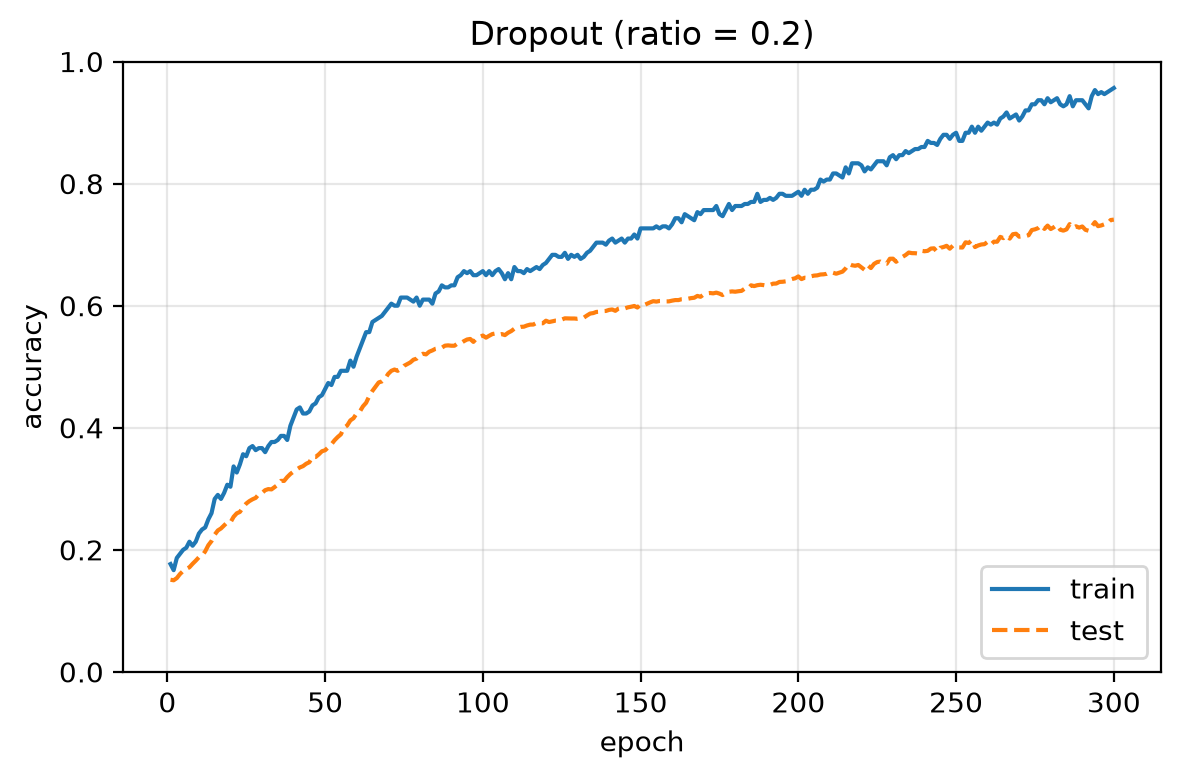
\includegraphics[width=0.62\textwidth]{figures/overfit_dropout.png}

\small 드롭아웃 ($p=0.2$)을 적용했을 때의 정확도
\end{center}
}{%
\begin{center}
\fbox{\parbox{0.8\textwidth}{\centering\small
[그림 자리] \texttt{figures/overfit\_dropout.png}\\
\texttt{mnist\_overfit.py}를 실행하면 생성된다.}}
\end{center}
}

\begin{center}
\begin{tabular}{@{}lcccc@{}}
\toprule
& \multicolumn{2}{c}{$200$ epoch} & \multicolumn{2}{c}{$300$ epoch} \\
\cmidrule(lr){2-3}\cmidrule(l){4-5}
& 훈련 & 시험 & 훈련 & 시험 \\
\midrule
규제 없음 & $100\%$ & $80.3\%$ & $100\%$ & $80.7\%$ \\
가중치 감소 ($\lambda=0.1$) & $85.3\%$ & $70.7\%$ & $85.7\%$ & $71.8\%$ \\
드롭아웃 ($p=0.2$) & $78.7\%$ & $64.8\%$ & $95.7\%$ & $74.1\%$ \\
\bottomrule
\end{tabular}
\end{center}

\begin{itemize}[leftmargin=1.8em]
\item 드롭아웃을 쓰면 훈련 정확도가 훨씬 천천히 올라간다.
매 단계 일부 node가 사라지므로 network가 훈련 데이터를 \textbf{외우기 어렵기} 때문이다.
학습하는 동안 훈련과 시험 정확도의 차이는 규제가 없을 때보다 작다 ($200$ epoch에서 $13.9\%$p).
\item 그러나 학습을 계속하면 결국 훈련 정확도가 $100\%$에 가까워지고 차이도 다시 벌어진다 ($300$ epoch에서 $21.6\%$p).
드롭아웃은 오버피팅을 \textbf{늦추고 억제}하지만, 데이터 $300$장으로 $13$만 개의 parameter를 학습하는 상황 자체를 바꾸지는 못한다.
\item 이 실험처럼 좁고 깊은 network에 데이터가 아주 적을 때는 드롭아웃의 효과가 크지 않다.
드롭아웃은 node가 많은 넓은 network를 충분한 데이터로 오래 학습할 때 효과적이다.
삭제 비율 $p$도 $\lambda$처럼 검증 데이터로 고르는 hyperparameter이다.
\end{itemize}

\begin{thinkbox}[드롭아웃과 앙상블 학습]
\textbf{앙상블 학습(ensemble learning)}은 여러 network를 따로 학습시켜 추론할 때 그 출력의 평균을 내는 방법으로,
성능을 몇 \% 개선하는 것으로 알려져 있다.
드롭아웃은 학습할 때마다 node를 무작위로 삭제하므로 매번 \textbf{다른 network}를 학습시키는 것으로 볼 수 있다.
node가 $n$개면 가능한 network는 $2^n$개이고, 이들은 가중치를 공유한다.
추론할 때 모든 node를 쓰고 크기를 보정하는 것은 이 수많은 network의 출력을 (근사적으로) 평균 내는 효과를 낸다.
즉 드롭아웃은 앙상블 학습을 \textbf{하나의 network로 흉내} 낸 것이다.
또 특정 node에 의존할 수 없으므로 각 node가 다른 node 없이도 쓸모 있는 특징을 배우게 된다.
\end{thinkbox}

\begin{remarkbox}[실무에서의 규제]
\begin{itemize}[leftmargin=1.5em]
\item PyTorch에서는 \texttt{nn.Dropout(p)}를 쓰고, \texttt{model.train()}과 \texttt{model.eval()}로 학습과 추론을 전환한다.
가중치 감소는 optimizer의 인자로 준다.
\begin{center}
\texttt{torch.optim.AdamW(model.parameters(), lr=1e-3, weight\_decay=0.01)}
\end{center}
\texttt{torch.optim.SGD}와 \texttt{torch.optim.Adam}의 \texttt{weight\_decay}는 L2 규제 방식이다.
\item 배치 정규화를 쓰는 CNN에서는 드롭아웃을 마지막 fully-connected 층에만 쓰거나 아예 쓰지 않는 경우가 많다.
배치 정규화 자체에 규제 효과가 있기 때문이다 (\ref{sec:bneffect}절).
\item Transformer에서는 $p=0.1$ 정도의 드롭아웃을 흔히 쓰지만,
데이터가 매우 많은 대규모 언어모델의 사전학습에서는 드롭아웃을 쓰지 않는 ($p=0$) 경우도 많다.
데이터가 충분하면 오버피팅 자체가 잘 일어나지 않기 때문이다.
\item 이 밖의 규제로 \textbf{데이터 증강(data augmentation)} (이미지를 회전, 이동, 반전하여 데이터를 늘림),
\textbf{조기 종료(early stopping)} (검증 정확도가 더 오르지 않으면 학습을 멈춤) 등이 있다.
\end{itemize}
\end{remarkbox}

\begin{keybox}[바른 학습을 위해: 정리]
\begin{itemize}[leftmargin=1.5em]
\item \textbf{오버피팅}: 훈련 데이터에만 맞추어져 처음 보는 데이터에서 성능이 떨어지는 현상.
훈련 정확도와 시험(검증) 정확도의 차이로 확인한다.
\item \textbf{가중치 감소}: 손실에 $\frac\lambda2\sum\lVert W\rVert^2$를 더한다. gradient에 $\lambda W$를 더하면 된다.
Adam에서는 감소를 분리한 \textbf{AdamW}를 쓴다.
\item \textbf{드롭아웃}: 학습할 때 node를 확률 $p$로 무작위 삭제하고, 추론할 때는 모든 node를 쓴다.
\item 규제의 세기 ($\lambda$, $p$)는 hyperparameter이며, \textbf{검증 데이터}로 고른다.
너무 강하면 과소적합이 된다.
\end{itemize}
\end{keybox}

% =================================================
\section{적절한 하이퍼파라미터 값 찾기}\label{sec:hyper}
% =================================================

신경망에는 가중치 $W$와 bias $B$ 말고도 사람이 정해 주어야 하는 값이 많다.
이런 값을 \textbf{하이퍼파라미터(hyperparameter)}라고 한다.

\begin{center}
\begin{tabular}{@{}p{0.2\textwidth}p{0.36\textwidth}p{0.36\textwidth}@{}}
\toprule
& 매개변수 (parameter) & 하이퍼파라미터 (hyperparameter) \\
\midrule
예 & $W$, $B$, 배치 정규화의 $\bm\gamma$, $\bm\beta$ &
학습률 $\alpha$, 가중치 감소 $\lambda$, 드롭아웃 비율 $p$, 미니배치 크기, epoch 수, 층의 수, 각 층의 node 수, 초깃값의 표준편차, optimizer의 $\beta_1$, $\beta_2$, $\ldots$ \\[3pt]
정하는 방법 & 훈련 데이터의 손실을 줄이도록 \textbf{gradient로 자동} 학습 & 학습 \textbf{전에} 사람이 정한다. 여러 값을 시도하여 비교한다. \\
\bottomrule
\end{tabular}
\end{center}

지금까지의 실험에서도 학습률을 $0.01$로 할지 $0.1$로 할지, $\lambda$를 얼마로 할지 계속 골라야 했다.
하이퍼파라미터를 잘못 고르면 같은 network라도 성능이 크게 떨어진다 (\ref{sec:mnistopt}절의 SGD, \ref{sec:weightdecay}절의 $\lambda=0.3$).
이 절에서는 하이퍼파라미터를 \textbf{무엇을 기준으로}, \textbf{어떻게} 고르는지 다룬다.

\subsection{검증 데이터}\label{sec:validation}

지금까지 우리는 데이터를 크게 두 그룹으로 나누어 생각했다.
\begin{itemize}[leftmargin=1.8em]
\item \textbf{훈련 데이터(training data)}: 매개변수 $W$, $B$를 학습하는 데 쓴다.
\item \textbf{시험 데이터(test data)}: 학습이 끝난 network의 \textbf{범용 성능}, 즉 처음 보는 데이터에 대한 성능을 평가하는 데 쓴다.
\end{itemize}
그렇다면 하이퍼파라미터의 좋고 나쁨은 무엇으로 평가해야 할까?

\paragraph{시험 데이터로 하이퍼파라미터를 고르면 안 된다.}
여러 하이퍼파라미터로 학습시킨 뒤 시험 정확도가 가장 높은 것을 고른다고 하자.
그러면 하이퍼파라미터가 \textbf{시험 데이터에 맞추어} 선택된다.
시험 데이터에도 우연한 특징이 있으므로, 그 우연에 잘 맞는 하이퍼파라미터가 뽑히게 되고,
이렇게 고른 network의 시험 정확도는 처음 보는 데이터에 대한 실제 성능보다 \textbf{높게 나온다}.
매개변수가 훈련 데이터에 오버피팅하듯이, 하이퍼파라미터가 시험 데이터에 오버피팅하는 것이다.
그러면 시험 데이터는 더 이상 ``처음 보는 데이터''의 역할을 할 수 없다.

그래서 하이퍼파라미터를 고르기 위한 데이터를 따로 둔다.
이것을 \textbf{검증 데이터(validation data)}라고 한다.

\begin{keybox}[훈련 / 검증 / 시험 데이터]
\begin{itemize}[leftmargin=1.5em]
\item \textbf{훈련 데이터}: 매개변수 ($W$, $B$, $\bm\gamma$, $\bm\beta$) 학습
\item \textbf{검증 데이터}: 하이퍼파라미터의 성능 평가와 선택
\item \textbf{시험 데이터}: 최종 선택한 network의 범용 성능 평가. \textbf{마지막에 단 한 번}만 쓴다.
\end{itemize}
\end{keybox}

시험 공부에 비유하면 훈련 데이터는 교재의 연습문제, 검증 데이터는 공부 방법을 점검하는 모의고사,
시험 데이터는 수능이다. 수능 문제를 미리 보고 공부 방법을 정하면 수능 점수는 실력을 나타내지 못한다.

\paragraph{검증 데이터는 훈련 데이터에서 떼어 낸다.}
MNIST처럼 훈련 데이터와 시험 데이터만 나누어져 있는 데이터셋이 많다.
이때는 훈련 데이터의 일부(보통 $10\sim20\%$)를 무작위로 골라 검증 데이터로 떼어 두고, 나머지만 학습에 쓴다.

\begin{center}
\begin{tikzpicture}[x=1.9mm,y=1mm]
\draw[thick,fill=blue!12] (0,0) rectangle (55,8);
\draw[thick,fill=orange!30] (55,0) rectangle (60,8);
\draw[thick,fill=black!12] (62,0) rectangle (72,8);
\node at (27.5,4) {\small 훈련 데이터 $55000$장};
\node[font=\scriptsize,align=center] at (57.5,4) {검증\\$5000$};
\node[font=\small,align=center] at (67,4) {시험\\$10000$장};
\draw[decorate,decoration={brace,amplitude=4pt}] (0,9.5) -- (60,9.5)
  node[midway,above=5pt,font=\small] {MNIST의 훈련 데이터 $60000$장};
\draw[decorate,decoration={brace,amplitude=4pt}] (62,9.5) -- (72,9.5)
  node[midway,above=5pt,font=\small] {MNIST의 시험 데이터};
\node[font=\scriptsize,anchor=north] at (27.5,-1) {$W$, $B$ 학습};
\node[font=\scriptsize,anchor=north,align=center] at (57.5,-1) {하이퍼파라미터\\선택};
\node[font=\scriptsize,anchor=north,align=center] at (67,-1) {마지막에\\한 번};
\end{tikzpicture}
\end{center}

이 강의의 \texttt{mnist\_data.py}가 바로 이렇게 나눈다.
지난주의 \texttt{mnist\_mlp.py} 과제에서 간단히 소개했던 분할과 같은 것이다.
\begin{lstlisting}
    # hold out n_val training images as a VALIDATION set
    perm = np.random.permutation(x_all.shape[0])
    val_idx, train_idx = perm[:n_val], perm[n_val:]
    return (x_all[train_idx], t_all[train_idx],
            x_all[val_idx], t_all[val_idx],
            x_test, t_test)
\end{lstlisting}
이 노트의 \ref{sec:mnistopt}, \ref{sec:mnistinit}, \ref{sec:bneffect}절에서 optimizer, 초깃값, 배치 정규화를 비교할 때
시험 정확도가 아니라 \textbf{검증 정확도}를 보고한 것도 이 때문이다.
여러 방법 중 무엇이 나은지 \textbf{고르는} 실험이었기 때문이다.
(\ref{sec:overfit}절에서 시험 데이터를 쓴 것은 고르기 위해서가 아니라 오버피팅 현상 자체를 보여 주기 위해서였다.)

\begin{remarkbox}[데이터가 적을 때: 교차 검증]
데이터가 아주 적으면 검증 데이터를 떼어 내기 아깝고, 검증 데이터가 작으면 검증 정확도 자체가 우연에 크게 흔들린다.
이럴 때는 훈련 데이터를 $K$개 묶음으로 나누어, 한 묶음을 검증 데이터로, 나머지를 훈련 데이터로 쓰는 실험을
$K$번 반복하고 검증 정확도를 평균하는 \textbf{$K$-겹 교차 검증($K$-fold cross validation)}을 쓴다.
비용이 $K$배이므로 데이터가 많은 딥러닝에서는 보통 하나의 검증 데이터만 둔다.
\end{remarkbox}

\subsection{하이퍼파라미터 최적화}\label{sec:hpo}

하이퍼파라미터는 gradient로 학습할 수 없으므로, 값을 바꾸어 가며 직접 학습시켜 보고 검증 정확도를 비교하는 수밖에 없다.
핵심은 \textbf{좋은 값이 있을 법한 범위를 점점 좁혀 가는 것}이다.

\begin{keybox}[하이퍼파라미터 최적화의 절차]
\begin{enumerate}[label=\textbf{\arabic*단계}, leftmargin=4.2em, start=0]
\item 하이퍼파라미터의 범위를 대략적으로 정한다 (예: 학습률 $10^{-5}\sim1$).
\item 그 범위에서 하이퍼파라미터 값을 \textbf{무작위로} 뽑는다.
\item 뽑은 값으로 학습하고 \textbf{검증 데이터}로 정확도를 평가한다. 이때 epoch은 작게 한다.
\item 1, 2단계를 일정 횟수 (예: $100$번) 반복하고, 정확도가 좋은 값들이 모인 곳으로 범위를 좁힌다.
\end{enumerate}
범위가 충분히 좁아지면 그 안에서 하나를 골라, 전체 데이터로 오래 학습한 뒤 시험 데이터로 최종 평가한다.
\end{keybox}

\paragraph{로그 눈금(log scale)으로 뽑는다.}
학습률이 $0.001$인지 $0.002$인지보다 $0.001$인지 $0.01$인지가 훨씬 중요하다.
하이퍼파라미터는 대개 \textbf{몇 배}가 차이 나는지가 중요하므로, 지수를 균등하게 뽑는다.
\[
\alpha=10^{u},\qquad u\sim\mathrm{Uniform}(-5,\,0)
\]
$\alpha$를 $10^{-5}$과 $1$ 사이에서 그냥 균등하게 뽑으면 $90\%$가 $0.1$보다 큰 값이 되어
작은 학습률은 거의 시험해 보지 못한다.

\paragraph{격자 탐색보다 무작위 탐색.}
값을 $\{10^{-4},10^{-3},10^{-2}\}$처럼 격자로 정해 모든 조합을 시험하는 \textbf{격자 탐색(grid search)}보다,
무작위로 뽑는 \textbf{무작위 탐색(random search)}이 대개 더 좋은 결과를 낸다 (Bergstra \& Bengio, 2012).
하이퍼파라미터들 중 결과에 큰 영향을 주는 것은 일부뿐이기 때문이다.
아래 그림에서 가로축이 중요한 하이퍼파라미터, 세로축이 거의 영향이 없는 하이퍼파라미터라고 하자.
똑같이 $9$번 시험해도 격자 탐색은 중요한 축에서 $3$가지 값만 보지만, 무작위 탐색은 $9$가지 값을 본다.

\begin{center}
\begin{tikzpicture}[x=3.2cm,y=3.2cm,>=Latex]
\foreach \dx/\name in {0/격자 탐색, 1.45/무작위 탐색}{
  \draw[thick] (\dx,0) rectangle (\dx+1,1);
  \draw[->] (\dx,-0.08) -- (\dx+1,-0.08) node[midway,below,font=\scriptsize] {중요한 하이퍼파라미터};
  \draw[->] (\dx-0.08,0) -- (\dx-0.08,1) node[midway,above,rotate=90,font=\scriptsize] {덜 중요한 하이퍼파라미터};
  \node[font=\small] at (\dx+0.5,1.48) {\name};
  \draw[domain=0:1,samples=60,smooth,thick,deepblue] plot ({\dx+\x},{1.12+0.22*exp(-((\x-0.62)^2)/0.012)});
}
\foreach \i in {1,2,3}{\foreach \j in {1,2,3}{
  \fill[orange!80!black] ({(\i-0.5)/3},{(\j-0.5)/3}) circle (0.025);}}
\foreach \i in {1,2,3}{\draw[orange!80!black,densely dotted] ({(\i-0.5)/3},1) -- ({(\i-0.5)/3},1.12);}
\foreach \x/\y in {0.08/0.62,0.21/0.18,0.33/0.85,0.44/0.41,0.57/0.73,0.64/0.12,0.71/0.53,0.83/0.92,0.93/0.29}{
  \fill[orange!80!black] (1.45+\x,\y) circle (0.025);
  \draw[orange!80!black,densely dotted] (1.45+\x,1) -- (1.45+\x,1.12);}
\end{tikzpicture}

\small 위의 곡선은 중요한 하이퍼파라미터에 따른 성능. 무작위 탐색은 봉우리 근처의 값을 시험할 기회가 많다.
\end{center}

\paragraph{시간을 줄이는 방법.}
하이퍼파라미터 하나를 평가하려면 network를 한 번 학습시켜야 하므로 시간이 많이 걸린다.
그래서 탐색 단계에서는 \textbf{데이터의 일부}와 \textbf{적은 epoch}으로 학습시켜
가망이 없는 값을 빨리 걸러 낸다. 좋은 범위를 찾은 뒤에 전체 데이터로 오래 학습한다.

\subsection{구현: 학습률과 가중치 감소의 무작위 탐색}\label{sec:hpocode}

\texttt{hyperparameter\_search.py}에서는 책에서와 같이 학습률 $\alpha$와 가중치 감소 $\lambda$ 두 가지를 무작위 탐색으로 찾는다.
시간을 줄이려고 훈련 데이터는 $500$장만 쓰고, $50$ epoch만 학습한다.
network는 \ref{sec:overfit}절과 같은 $7$층 network (은닉층 $6$개, 각 $100$개 node, He 초깃값, SGD)이다.
평가는 검증 데이터 $5000$장으로 한다.
\begin{lstlisting}
x_train, t_train, x_val, t_val, x_test, t_test = load_mnist_split()   # 55000 / 5000 / 10000
x_train, t_train = x_train[:500], t_train[:500]   # a small training set -> fast trials
\end{lstlisting}
\begin{lstlisting}
        train_acc.append(net.accuracy(x_train, t_train))
        val_acc.append(net.accuracy(x_val, t_val))   # VALIDATION data, not test data
\end{lstlisting}
학습률은 $10^{-5}\sim1$, 가중치 감소는 $10^{-6}\sim10^{-1}$의 범위에서 로그 눈금으로 $100$번 뽑는다.
\begin{lstlisting}
n_trials = 100
rng = np.random.default_rng(0)                    # separate random numbers for the sampling
results = []
for trial in range(n_trials):
    lr = 10 ** rng.uniform(-5, 0)                 # 1e-5 ~ 1
    weight_decay = 10 ** rng.uniform(-6, -1)      # 1e-6 ~ 0.1
    _, train_acc, val_acc = train(lr, weight_decay)
    results.append({"lr": lr, "wd": weight_decay, "train": train_acc, "val": val_acc})
\end{lstlisting}
모든 시행에서 초깃값과 미니배치 순서는 같게 하여 하이퍼파라미터의 차이만 비교한다.

\paragraph{결과.}
$100$번의 시행을 학습률과 가중치 감소의 평면에 찍고, 검증 정확도로 색을 칠하면 다음과 같다.

\IfFileExists{figures/hyper_scatter.png}{%
\begin{center}
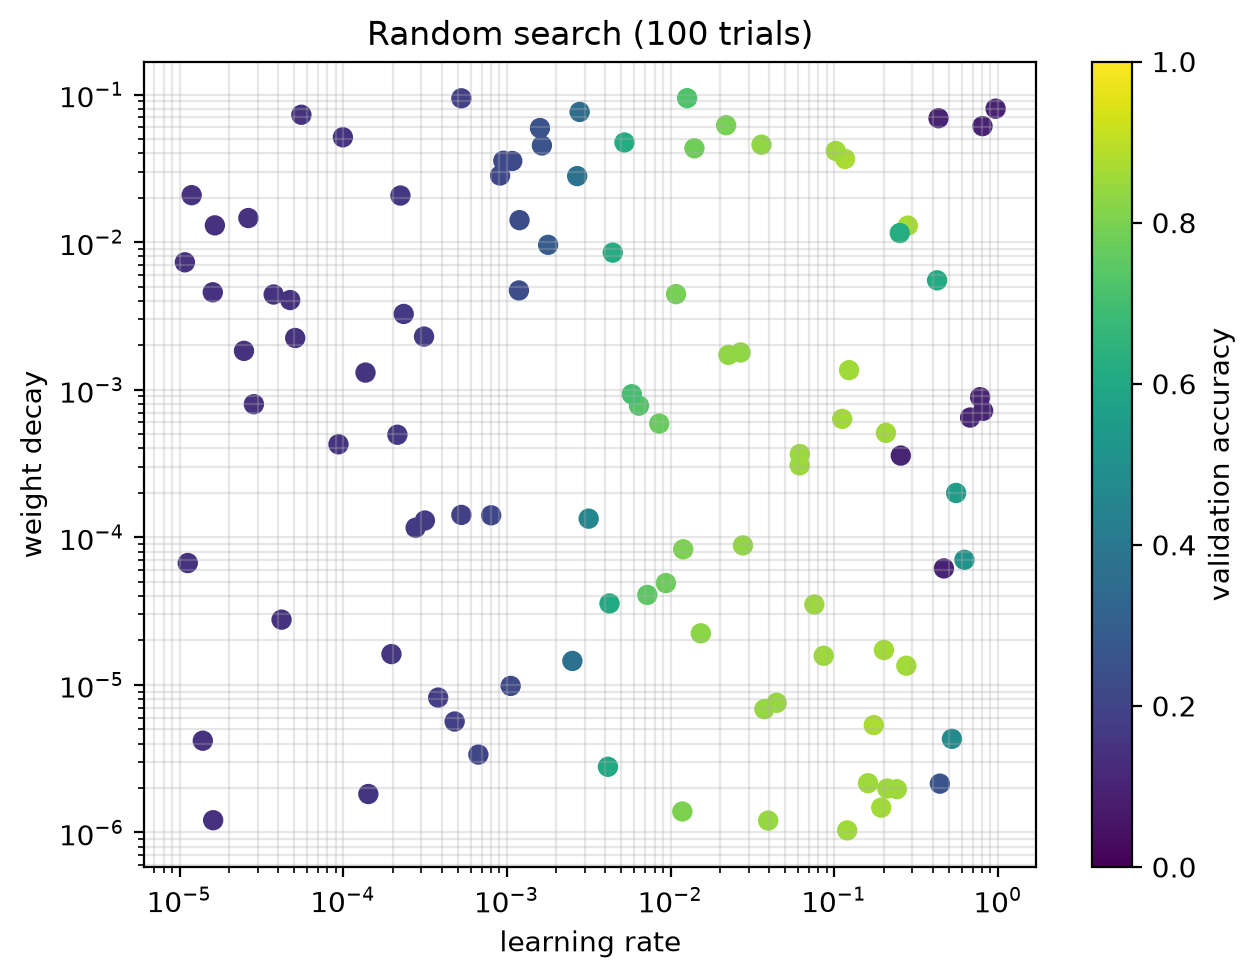
\includegraphics[width=0.66\textwidth]{figures/hyper_scatter.png}

\small 무작위 탐색 $100$번의 결과. 점 하나가 하나의 시행이고, 색이 밝을수록 검증 정확도가 높다.
\end{center}
}{%
\begin{center}
\fbox{\parbox{0.8\textwidth}{\centering\small
[그림 자리] \texttt{figures/hyper\_scatter.png}\\
\texttt{hyperparameter\_search.py}를 실행하면 생성된다.}}
\end{center}
}

학습률 구간별로 정리하면 다음과 같다.
\begin{lstlisting}
print("======= by learning rate =======")
edges = [1e-5, 1e-3, 1e-2, 3e-2, 1e-1, 3e-1, 1.0]
for lo, hi in zip(edges[:-1], edges[1:]):
    accs = [r["val"][-1] for r in results if lo <= r["lr"] < hi]
    print(f"lr {lo:.0e} ~ {hi:.0e}: {len(accs):3d} trials  best {max(accs):.4f}  mean {np.mean(accs):.4f}")
\end{lstlisting}

\begin{center}
\begin{tabular}{@{}lcccccc@{}}
\toprule
학습률 & $10^{-5}\sim10^{-3}$ & $10^{-3}\sim10^{-2}$ & $0.01\sim0.03$ & $0.03\sim0.1$ & $0.1\sim0.3$ & $0.3\sim1$ \\
\midrule
시행 수 & $34$ & $20$ & $10$ & $8$ & $16$ & $12$ \\
최고 검증 정확도 & $22.0\%$ & $77.6\%$ & $83.5\%$ & $85.5\%$ & $\mathbf{87.1\%}$ & $60.6\%$ \\
평균 검증 정확도 & $16.3\%$ & $47.2\%$ & $80.2\%$ & $\mathbf{84.7\%}$ & $79.8\%$ & $25.7\%$ \\
\bottomrule
\end{tabular}
\end{center}

\begin{itemize}[leftmargin=1.8em]
\item \textbf{학습률이 결과를 거의 결정한다.} 그림의 색이 가로 방향(학습률)으로는 크게 변하지만
세로 방향(가중치 감소)으로는 거의 변하지 않는다.
학습률이 $10^{-3}$보다 작으면 $50$ epoch 동안 거의 학습되지 않고,
$0.3$보다 크면 학습이 발산하여 정확도가 $10\%$ 근처로 떨어진다.
\item \textbf{가중치 감소는 $10^{-6}\sim10^{-2}$ 범위에서 거의 영향이 없다.}
이 범위에서는 감소량이 학습률에 비해 너무 작기 때문이다.
$\lambda$가 $5\times10^{-2}$ 이상이 되어야 정확도가 조금씩 떨어지기 시작한다.
앞에서 본 격자 탐색과 무작위 탐색의 그림에서 ``덜 중요한 하이퍼파라미터''가 바로 이런 경우이다.
무작위 탐색 덕분에 $100$번의 시행이 모두 서로 다른 학습률을 시험하였다.
\item 지금까지 SGD의 학습률로 $0.01$을 써 왔는데, 이 network에는 $0.1$ 근처가 더 좋다.
하이퍼파라미터의 좋은 값은 network와 데이터에 따라 다르므로 매번 찾아야 한다.
\end{itemize}

검증 정확도가 높은 상위 $20$개 시행의 학습 곡선은 다음과 같다.

\IfFileExists{figures/hyper_top20.png}{%
\begin{center}
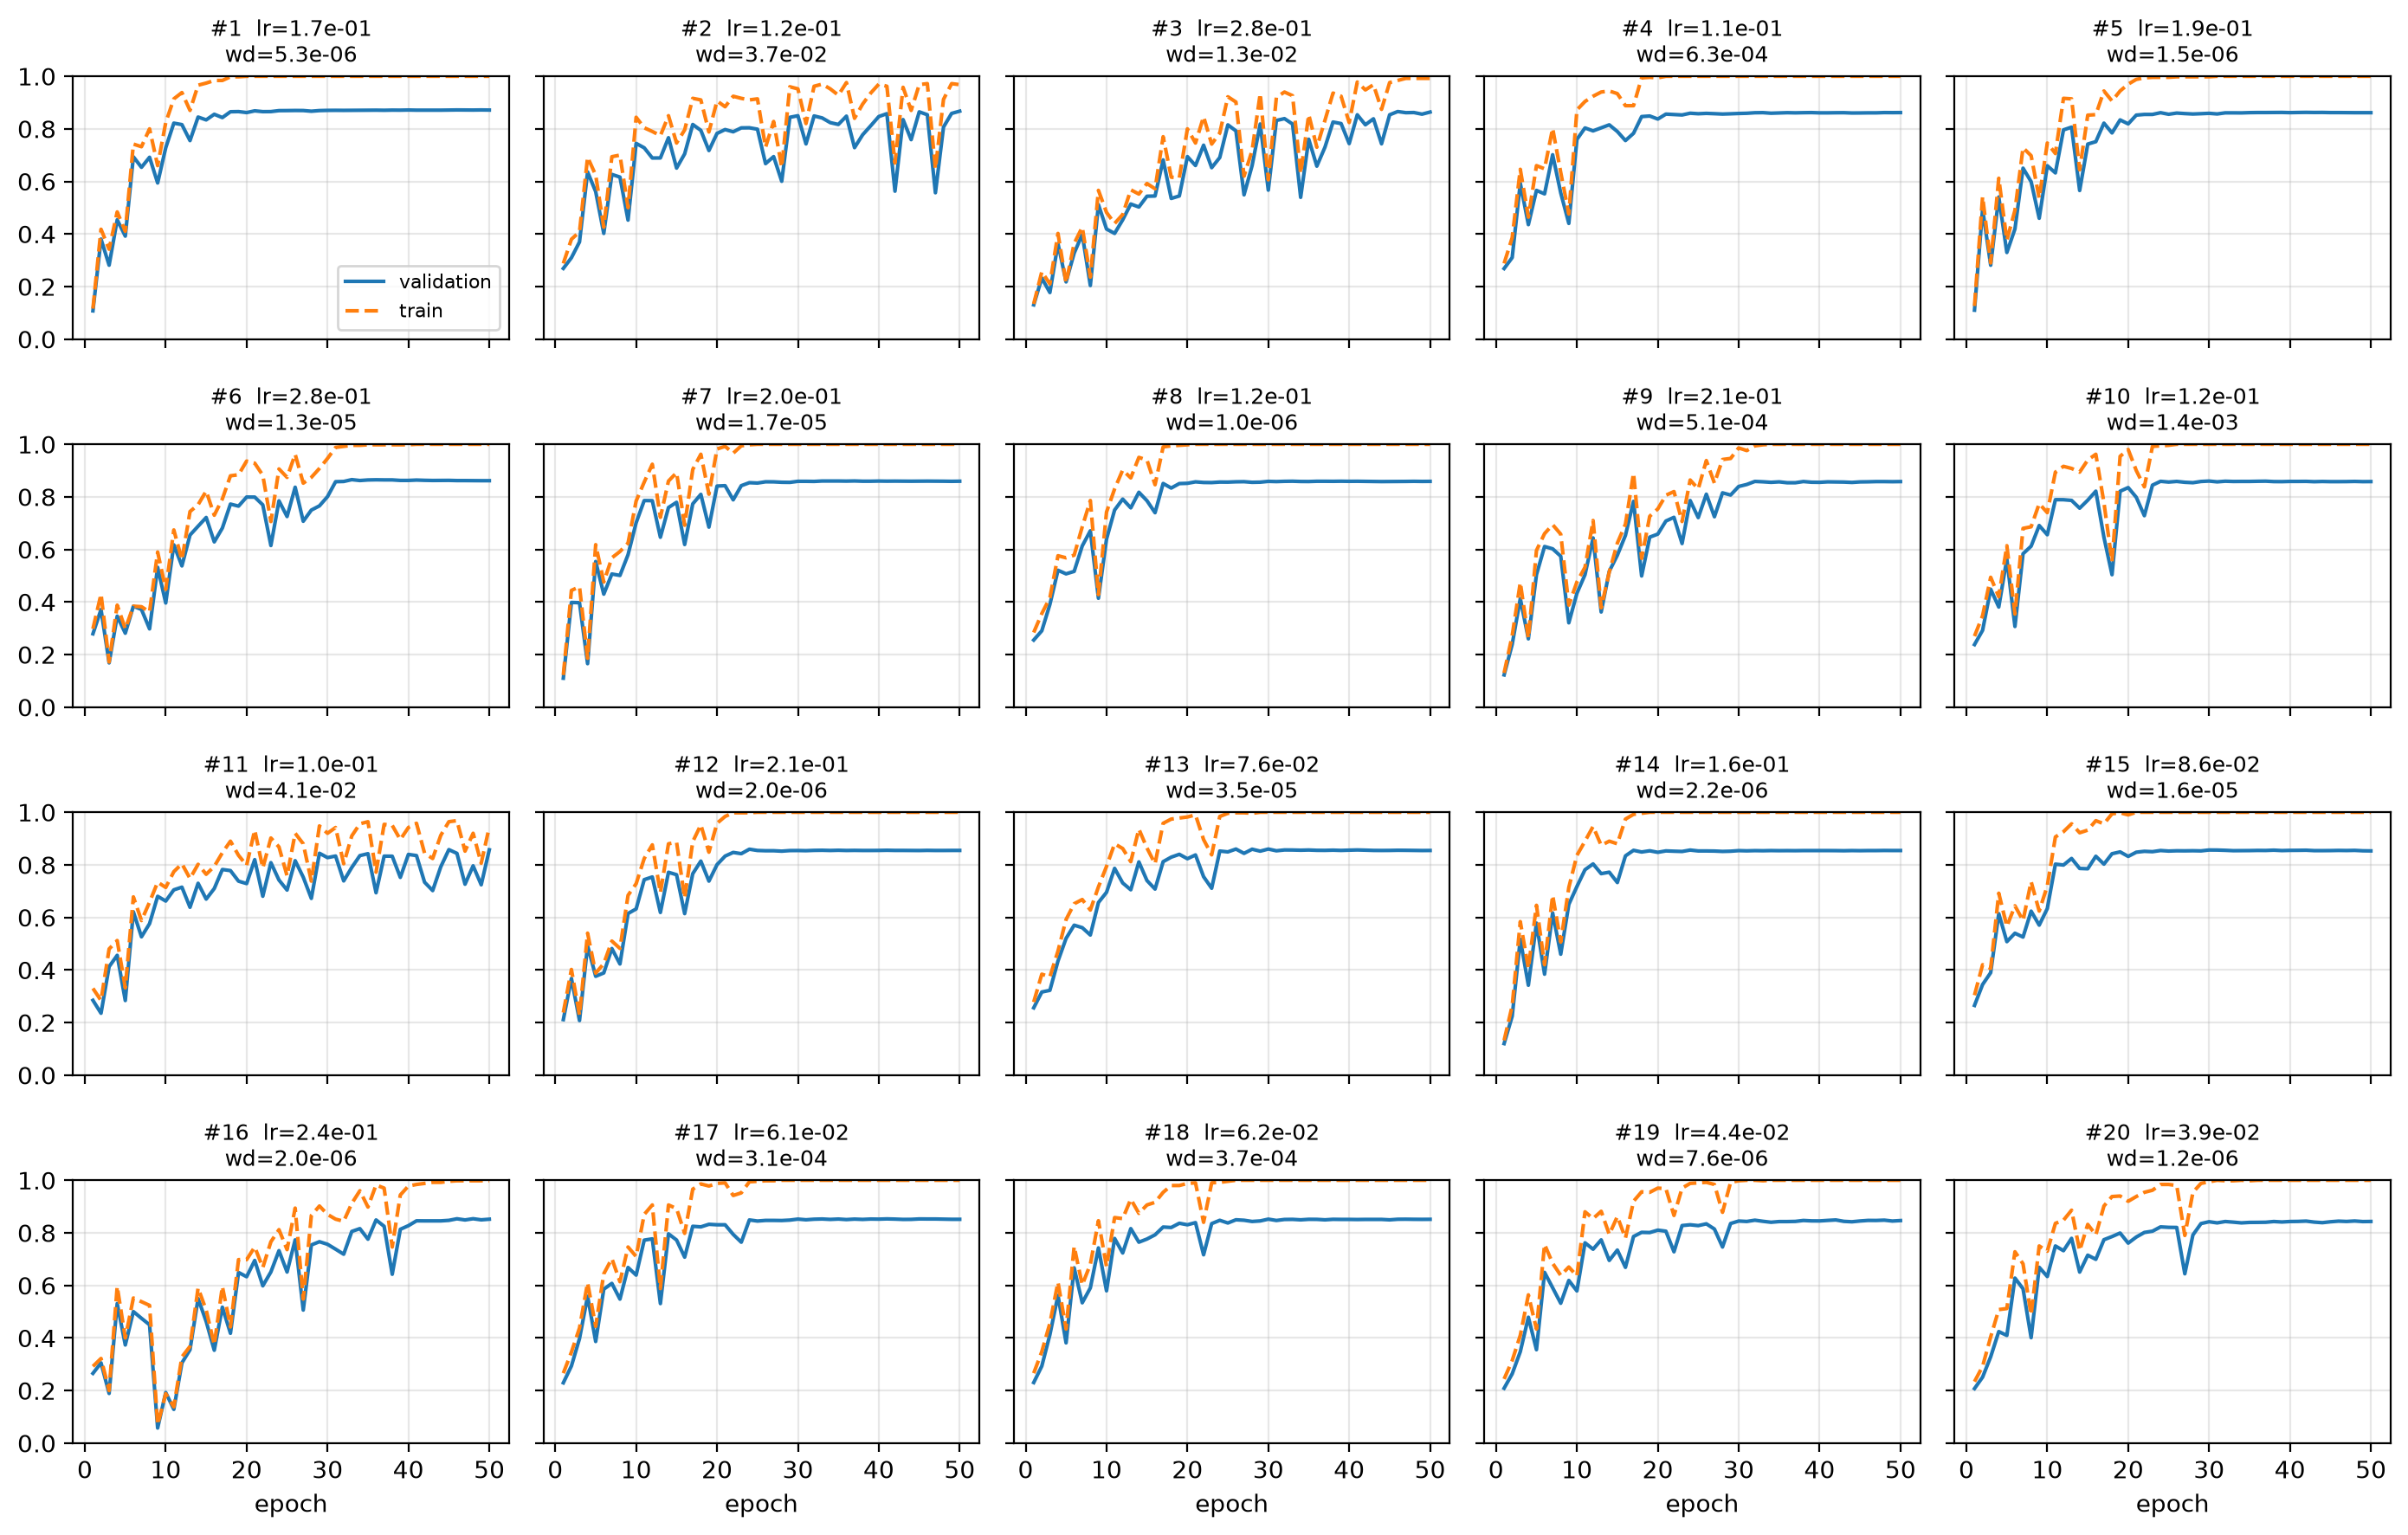
\includegraphics[width=\textwidth]{figures/hyper_top20.png}

\small 검증 정확도 상위 $20$개 시행의 학습 곡선 (실선: 검증, 점선: 훈련)
\end{center}
}{%
\begin{center}
\fbox{\parbox{0.8\textwidth}{\centering\small
[그림 자리] \texttt{figures/hyper\_top20.png}\\
\texttt{hyperparameter\_search.py}를 실행하면 생성된다.}}
\end{center}
}

\begin{center}
\begin{tabular}{@{}ccccc@{}}
\toprule
순위 & 검증 정확도 & 훈련 정확도 & 학습률 & 가중치 감소 \\
\midrule
1 & $87.1\%$ & $100\%$ & $1.7\times10^{-1}$ & $5.3\times10^{-6}$ \\
2 & $86.7\%$ & $96.8\%$ & $1.2\times10^{-1}$ & $3.7\times10^{-2}$ \\
3 & $86.4\%$ & $99.2\%$ & $2.8\times10^{-1}$ & $1.3\times10^{-2}$ \\
4 & $86.2\%$ & $100\%$ & $1.1\times10^{-1}$ & $6.3\times10^{-4}$ \\
5 & $86.1\%$ & $100\%$ & $1.9\times10^{-1}$ & $1.5\times10^{-6}$ \\
\bottomrule
\end{tabular}
\end{center}

\begin{itemize}[leftmargin=1.8em]
\item 상위 $10$개는 모두 학습률이 $0.11\sim0.28$이지만, 가중치 감소는 $10^{-6}$부터 $4\times10^{-2}$까지 흩어져 있다.
\item 학습률이 큰 쪽 ($2$위, $3$위)은 학습 곡선이 크게 흔들린다. 마지막 epoch의 정확도가 우연히 높게 나왔을 수도 있다.
\item 검증 데이터가 $5000$장이면 정확도 $87\%$의 표준오차는 $\sqrt{0.87\times0.13/5000}\approx0.5\%$p이다.
상위권의 $1\%$p 정도의 차이는 우연과 구별하기 어렵다.
그래서 $1$등 하나를 고르기보다 \textbf{좋은 값들이 모여 있는 범위}를 찾는 것이 중요하다.
\end{itemize}

\paragraph{범위 좁히기.}
이 결과로부터 다음 탐색의 범위를 학습률 $0.03\sim0.3$, 가중치 감소 $10^{-6}\sim10^{-2}$ 정도로 좁힐 수 있다.
좁힌 범위에서 다시 무작위 탐색을 하고, 필요하면 훈련 데이터와 epoch을 늘려 가며 이 과정을 반복한다.

\paragraph{마지막에 단 한 번: 시험 데이터.}
하이퍼파라미터를 정한 뒤에야 비로소 시험 데이터를 쓴다.
\begin{lstlisting}
best = results[0]
net, _, _ = train(best["lr"], best["wd"])
print(f"chosen: lr {best['lr']:.2e}, weight decay {best['wd']:.2e}  ->  "
      f"validation {best['val'][-1]:.4f}, test {net.accuracy(x_test, t_test):.4f}")
\end{lstlisting}
\begin{lstlisting}[language={},numbers=none]
chosen: lr 1.74e-01, weight decay 5.34e-06  ->  validation 0.8714, test 0.8701
\end{lstlisting}
검증 정확도 $87.1\%$와 시험 정확도 $87.0\%$가 거의 같다.
여기서는 차이가 작았지만, 일반적으로 $100$개 중 검증 정확도가 \textbf{가장 높은} 것을 골랐으므로
검증 정확도는 실제 성능보다 약간 높게 나오는 경향이 있다.
그래서 최종 성능은 반드시 선택에 쓰지 않은 시험 데이터로 보고한다.
이 시험 정확도를 본 뒤에 다시 하이퍼파라미터를 바꾸면 시험 데이터도 ``검증 데이터''가 되어 버린다.

\begin{remarkbox}[실무에서의 하이퍼파라미터 탐색]
\begin{itemize}[leftmargin=1.5em]
\item 가장 먼저, 가장 꼼꼼하게 찾아야 하는 것은 \textbf{학습률}이다.
그다음이 미니배치 크기, 가중치 감소, 드롭아웃 비율, network의 크기 등이다.
\item 이전 시행의 결과를 보고 다음에 시험할 값을 똑똑하게 고르는 \textbf{베이즈 최적화(Bayesian optimization)},
가망 없는 시행을 일찍 중단하여 시간을 아끼는 \textbf{Hyperband} 같은 방법이 있다.
Python에서는 \texttt{Optuna} 같은 라이브러리로 쉽게 쓸 수 있다.
\item 대규모 모델은 한 번 학습하는 데 며칠이 걸리므로 탐색을 많이 할 수 없다.
그래서 작은 모델에서 찾은 하이퍼파라미터를 큰 모델로 옮기는 방법,
논문과 공개된 설정에서 출발하는 방법을 많이 쓴다.
\item 검증 정확도가 더 오르지 않을 때 학습을 멈추는 \textbf{조기 종료}에서도 epoch 수라는 하이퍼파라미터를 검증 데이터로 정하는 것이다.
\end{itemize}
\end{remarkbox}

\begin{keybox}[하이퍼파라미터 찾기: 정리]
\begin{itemize}[leftmargin=1.5em]
\item 하이퍼파라미터는 \textbf{검증 데이터}로 고른다. 시험 데이터는 마지막에 한 번만 쓴다.
\item 검증 데이터는 훈련 데이터의 일부를 떼어 만든다 (MNIST: $55000$ / $5000$ / $10000$).
\item 범위를 넓게 잡고, \textbf{로그 눈금}으로 \textbf{무작위} 탐색하며, 좋은 값이 모인 곳으로 범위를 좁힌다.
\item 탐색 단계에서는 데이터와 epoch을 줄여 시간을 아낀다.
\end{itemize}
\end{keybox}

% =================================================
\section{연습문제}
% =================================================

\begin{enumerate}[label=\arabic*.]

\item $f(x,y)=\frac{1}{20}x^2+y^2$에서 SGD가 발산하지 않는 학습률 $\alpha$의 범위를 구하라.
또 이 범위 안에서 $x$ 방향의 수렴이 가장 빠른 $\alpha$와 그때 $x$가 한 단계에 몇 배가 되는지 구하라.

\item 모멘텀에서 gradient가 매 단계 같은 값 $g$로 일정하다고 하자.
$v_0=0$일 때 $v_k$를 구하고, $k\to\infty$일 때 $v_k\to-\dfrac{\alpha}{1-\beta}\,g$임을 보이라.

\item 시작점 $(-7,2)$에서 AdaGrad ($\alpha=1.5$)로 두 번째 단계 $(x_2,y_2)$를 손으로 계산하라
($\varepsilon$은 무시한다). 표의 값 $(-4.573,\ 0.136)$과 비교하라.

\item Adam에서 편향 보정을 하지 않으면 첫 단계의 이동량은 얼마가 되는가?
($\beta_1=0.9$, $\beta_2=0.999$, $\varepsilon$은 무시한다.) 편향 보정이 왜 필요한지 설명하라.

\item \texttt{mnist\_optimizer\_compare.py}에서 SGD의 학습률을 $0.01$에서 $0.05$, $0.1$로 바꾸어 보라.
SGD도 plateau를 빠져나오는가? 같은 조건에서 RMSProp ($\alpha=0.001$)을 \texttt{optimizers}에 추가하여
네 기법과 비교하라.

\item 은닉층의 모든 가중치를 같은 값 $c$로 초기화하면 학습이 진행되어도 은닉층의 node들이
계속 같은 값을 가지는 이유를 역전파 식 $\pd{L}{W}=X\T\pd{L}{A}$를 이용하여 설명하라.

\item $a=\sum_{i=1}^{n}z_iw_i$에서 $z_i=\max(0,a_i')$이고 $a_i'$이 평균 $0$인 대칭 분포를 따를 때
$\mathbb E[z_i^2]=\frac12\mathrm{Var}(a_i')$임을 보이고, 이로부터 He 초깃값 $\mathrm{Var}(w)=\frac2n$을 유도하라.

\item \texttt{weight\_init\_activation.py}에서 층의 수를 $5$에서 $20$으로 늘려
ReLU + Xavier와 ReLU + He의 마지막 층 활성화값의 표준편차를 비교하라.
Xavier에서 표준편차가 층마다 약 몇 배씩 줄어드는가?

\item 배치 정규화의 순전파 식 \eqref{eq:bnmu}--\eqref{eq:bny}를 보고,
같은 미니배치에서 Affine 계층의 가중치 $W$를 $a$배 ($a>0$) 하면 BatchNorm 계층의 출력 $Y$가 변하지 않음을 보이라
($\varepsilon$은 무시한다). 이 사실로부터 $\pd{L}{(aW)}=\frac1a\pd{L}{W}$임을 설명하라.

\item \ref{sec:bngraph}절의 단계 \ding{173}--\ding{178}을 모두 대입하여
remarkbox의 식 $\pd{L}{x_i}=\frac{1}{\sqrt{\sigma_B^2+\varepsilon}}\bigl(g_i-\bar g-\hat x_i\,\overline{g\hat x}\bigr)$을 유도하라.
($\bar g$, $\overline{g\hat x}$는 각각 $g_k$, $g_k\hat x_k$의 미니배치 평균이다.)

\item \texttt{mnist\_batchnorm.py}의 실험 2에서 \texttt{accuracy}가 이동평균 대신 미니배치 통계를 쓰도록
(\texttt{train\_flg=True}) 바꾸고, 검증 데이터를 $1$장씩 넣어 정확도를 계산해 보라.
어떤 일이 생기는가? 왜 그런가?

\item 가중치 감소를 적용한 SGD의 갱신식이 $W\leftarrow(1-\alpha\lambda)W-\alpha\pd{L}{W}$임을 보이라.
$\alpha=0.01$, $\lambda=0.1$일 때 gradient가 $0$이라면 $W$가 처음 값의 절반이 되기까지 몇 번의 갱신이 필요한가?

\item 하나의 parameter $w$에 대하여 gradient가 매 단계 $g$로 일정하다고 하자 ($g\neq0$, $\varepsilon$은 무시).
Adam에 L2 규제를 쓰면 감소 항 $\lambda w$가 실제 갱신량에 주는 영향이 $|g|$에 따라 어떻게 달라지는지,
AdamW와 비교하여 설명하라.

\item inverted dropout에서 학습할 때의 출력 $y=z\,M/(1-p)$의 기댓값이 $z$임을 보이라
($M$은 확률 $1-p$로 $1$, 확률 $p$로 $0$).
책의 방법 (학습할 때 $z\,M$, 추론할 때 $(1-p)z$)과 inverted dropout이 같은 network를 학습시킴을 설명하라.

\item \texttt{mnist\_overfit.py}에서 은닉층을 $[100]\times6$ 대신 $[500, 500]$으로 바꾸고,
드롭아웃의 삭제 비율 $p=0,\ 0.2,\ 0.5$를 \textbf{검증 데이터}로 비교하라.
어떤 $p$를 고르겠는가? 그 $p$로 학습한 network의 시험 정확도를 보고하라.

\item 하이퍼파라미터 $10$개를 시험하여 시험 정확도가 가장 높은 것을 골랐더니 시험 정확도가 $98\%$였다.
이 $98\%$를 처음 보는 데이터에 대한 성능이라고 보고해도 되는가? 왜 그런가? 어떻게 해야 하는가?

\item 학습률 $\alpha$를 $[10^{-5},\,1]$에서 (a) 그냥 균등하게, (b) $\alpha=10^{u}$, $u\sim\mathrm{Uniform}(-5,0)$으로 뽑을 때,
$\alpha<10^{-2}$일 확률을 각각 구하라.

\item \texttt{hyperparameter\_search.py}의 결과를 보고 학습률과 가중치 감소의 범위를 좁혀
($100$번 대신 $30$번) 다시 탐색하라. 좁힌 범위와 그 근거, 가장 좋은 검증 정확도를 표로 정리하라.

\end{enumerate}

% =================================================
\appendix
\section{부록: 실제 딥러닝의 optimizer와 2차 미분을 쓰는 방법}\label{app:opt}
% =================================================

본문에서는 SGD, 모멘텀, AdaGrad, RMSProp, Adam의 원리를 살펴보았다.
이 부록에서는 두 가지 질문을 다룬다.
\begin{enumerate}[label=(\arabic*)]
\item 요즘 실제 딥러닝에서는 어떤 optimizer가 쓰이는가?
\item ``Gradient Descent와 Newton's method'' 시간에 본 Newton 방법처럼
\textbf{2차 미분(곡률) 정보}를 쓰는 방법은 딥러닝에서 어떻게 되는가?
\end{enumerate}
이 부록에서는 매개변수 전체를 한 줄로 펼친 열벡터 $\theta\in\R^n$으로 쓰고,
$g_k=\nabla L(\theta_k)$, Hessian을 $H=\nabla^2L$로 쓴다.

\begin{remarkbox}[이 부록을 읽는 방법]
이 부록은 시험 범위가 아니라 \textbf{읽을거리}이다.
Armijo $\cdot$ Wolfe 조건, BFGS 갱신식, two-loop recursion 같은 세부 수식은
최적화 이론(수치최적화) 과목에서 자세히 다루는 내용이므로 지금 모두 이해하지 않아도 된다.
대신 다음 두 가지에 집중해서 읽자.
\begin{itemize}[leftmargin=1.5em]
\item 각 방법이 \textbf{무엇을 근사하려고 하는가} (대부분 Hessian, 즉 곡률 정보이다)
\item 그 방법이 딥러닝에서 \textbf{왜 잘 쓰이는가, 또는 왜 잘 쓰이지 않는가}
\end{itemize}
이번 주에 배운 SGD와 Adam 너머에 어떤 최적화 이론이 있고,
그것이 지금도 딥러닝 연구에 어떻게 적용되고 있는지 감을 잡는 것이 목표이다.
\end{remarkbox}

% -------------------------------------------------
\subsection{요즘 실제로 쓰이는 optimizer}
% -------------------------------------------------

본문의 기법들이 모두 같은 비중으로 쓰이는 것은 아니다.
대략적인 경향은 다음과 같다.

\begin{center}
\begin{tabular}{@{}lp{0.68\textwidth}@{}}
\toprule
optimizer & 주로 쓰이는 곳 \\
\midrule
\textbf{AdamW} & 사실상의 기본값. Transformer, 대규모 언어모델(LLM), 확산(diffusion) 모델 등 최신 모델 대부분 \\[3pt]
\textbf{SGD + 모멘텀} & 이미지 분류 CNN (ResNet 등). 잘 조정하면 일반화 성능이 Adam보다 좋은 경우가 많다.
Nesterov 모멘텀을 함께 쓰기도 한다. \\[3pt]
Adam & AdamW 이전의 표준. 작은 모델과 실습에서는 여전히 많이 쓰인다. \\[3pt]
RMSProp & 예전에 강화학습(DQN 등)과 RNN에서 많이 쓰였으나 비중이 줄었다. \\[3pt]
AdaGrad & 추천 시스템처럼 희소한(sparse) 특징이 많은 문제 정도에서 쓰인다. \\
\bottomrule
\end{tabular}
\end{center}

\paragraph{AdaGrad는 왜 배우는가?}
AdaGrad는 지금 거의 쓰이지 않지만, ``\textbf{매개변수마다 학습률을 다르게}''라는 아이디어의 출발점이다.
그 약점을 고친 것이 RMSProp이고, RMSProp에 모멘텀을 합친 것이 Adam이다.
즉 AdaGrad $\rightarrow$ RMSProp $\rightarrow$ Adam $\rightarrow$ AdamW로 이어지는 흐름을 이해하기 위해 배운다.

\paragraph{AdamW.}
Adam에 \textbf{weight decay(가중치 감소)}를 올바르게 붙인 방법이다 (Loshchilov \& Hutter, 2019).
Adam의 손실에 L2 정규화 항을 그냥 더하면 그 항의 gradient도 $\sqrt{\hat v}$로 나뉘어,
정규화의 세기가 매개변수마다 들쭉날쭉해진다.
AdamW는 감소 항을 갱신식에서 따로 떼어 적용한다.
갱신식과 코드는 \ref{sec:adamw}절에서 살펴보았다.

\paragraph{최근에 연구되고 쓰이는 방법들.}
아직 AdamW만큼 표준은 아니지만 다음과 같은 방법들이 있다.
\begin{itemize}[leftmargin=1.8em]
\item \textbf{Lion} (2023): gradient의 \textbf{부호}만 사용해 갱신하여 메모리를 아낀다.
\item \textbf{Adafactor}: Adam의 2차 moment $v$를 행과 열의 통계로 압축해 메모리를 아낀다. 큰 언어모델 학습에 쓰였다.
\item \textbf{LAMB, LARS}: 층마다 갱신량의 크기를 조절하여 \textbf{아주 큰 미니배치}로 학습할 때 쓴다.
\item \textbf{Shampoo, Muon}: 가중치 행렬의 구조를 이용해 곡률을 근사하는 방법 (\ref{app:largescale}절).
\end{itemize}

\paragraph{optimizer보다 중요할 때가 많은 것: 학습률 스케줄.}
실무에서는 어떤 optimizer를 고르느냐보다 \textbf{학습률을 단계에 따라 어떻게 바꾸느냐}가
성능에 더 큰 영향을 주는 경우가 많다. 대표적인 것은
처음 $K_w$단계 동안 학습률을 $0$에서 서서히 올리는 \textbf{warmup}과,
그 뒤 남은 $K$단계 동안 학습률을 코사인 곡선을 따라 줄이는 \textbf{cosine 감소}이다.
\[
\alpha_k=
\begin{cases}
\alpha_{\max}\,\dfrac{k}{K_w}, & 0\le k<K_w\\[10pt]
\alpha_{\min}+\dfrac12\bigl(\alpha_{\max}-\alpha_{\min}\bigr)\Bigl(1+\cos\dfrac{\pi\,(k-K_w)}{K}\Bigr), & K_w\le k\le K_w+K
\end{cases}
\]
처음에는 아직 $m$, $v$ 같은 통계가 불안정하므로 작은 보폭으로 시작하고,
마지막에는 보폭을 줄여 최솟값 근처에서 흔들리지 않게 한다
(본문의 RMSProp 그림에서 최솟값 근처의 흔들림을 떠올려 보자).
weight decay의 세기와 함께 이 스케줄이 최종 성능을 크게 좌우한다.

% -------------------------------------------------
\subsection{SGD는 언제 수렴하는가?}\label{app:sgdconv}
% -------------------------------------------------

``Gradient Descent와 Newton's method'' 시간에는 정확한 gradient를 쓰는 경사하강법이
$|1-\alpha f''|<1$이면 수렴함을 보았고, 본문 \ref{sec:sgd}절에서도 같은 조건을 확인하였다.
그런데 실제 SGD는 \textbf{미니배치}로 gradient를 계산하므로 gradient에 \textbf{잡음}이 섞인다.
잡음이 있어도 수렴할까? 학습률은 어떻게 정해야 할까?

\paragraph{1. 가정: 잡음이 섞인 gradient.}
$k$번째 단계에서 실제로 쓰는 gradient를
\[
\hat g_k=\nabla L(\theta_k)+\xi_k
\]
라 하자. 잡음 $\xi_k$에 대해 다음을 가정한다.
\[
\mathbb E[\xi_k\mid\theta_k]=0\quad(\text{평균적으로 정확한 gradient}),
\qquad
\mathbb E\bigl[\|\xi_k\|^2\mid\theta_k\bigr]\le\sigma^2\quad(\text{잡음의 크기는 유한}).
\]
미니배치 gradient는 데이터별 gradient의 평균이므로 첫 번째 조건을 만족하고,
미니배치 크기가 $h$이면 평균의 분산이므로 대략 $\sigma^2\propto\frac1h$이다
(미니배치가 클수록 잡음이 작다).

또 손실함수의 \textbf{곡률이 어디서나 $M$ 이하}라고 가정한다
(정확히는 $\|\nabla L(a)-\nabla L(b)\|\le M\|a-b\|$, 이를 $M$-smooth라 한다).
2차 함수에서 $M$은 Hessian의 가장 큰 고유값이고, 본문의 예제에서는 $M=2$이다.
이 가정에서 Taylor 전개의 상한
\[
L(\theta')\le L(\theta)+\nabla L(\theta)\T(\theta'-\theta)+\frac M2\|\theta'-\theta\|^2
\tag{A.1}
\]
가 성립한다.

\paragraph{2. 잡음이 없을 때: $\alpha<2/M$.}
(A.1)에 $\theta'=\theta_k-\alpha\nabla L(\theta_k)$를 넣으면
\[
L(\theta_{k+1})\le L(\theta_k)-\alpha\Bigl(1-\frac{M\alpha}{2}\Bigr)\|\nabla L(\theta_k)\|^2
\]
이다. 따라서 $0<\alpha<\frac2M$이면 매 단계 손실이 줄어든다.
예제에서는 $M=2$이므로 $\alpha<1$, 본문의 SGD 분석 결과($y$ 방향이 발산하지 않을 조건)와 같다.

\paragraph{3. 잡음이 있을 때: 한 단계의 기댓값.}
(A.1)에 $\theta'=\theta_k-\alpha\hat g_k$를 넣고 $\theta_k$가 주어졌을 때의 기댓값을 취하면,
$\mathbb E[\hat g_k]=\nabla L(\theta_k)$와
$\mathbb E\|\hat g_k\|^2=\|\nabla L(\theta_k)\|^2+\mathbb E\|\xi_k\|^2\le\|\nabla L(\theta_k)\|^2+\sigma^2$에서
\[
\boxed{
\mathbb E\bigl[L(\theta_{k+1})\mid\theta_k\bigr]
\le L(\theta_k)
-\underbrace{\alpha\Bigl(1-\frac{M\alpha}{2}\Bigr)\|\nabla L(\theta_k)\|^2}_{\text{gradient에 의한 감소}}
+\underbrace{\frac{M\alpha^2\sigma^2}{2}}_{\text{잡음에 의한 증가}}
}
\]
를 얻는다.
최솟값에 가까워지면 $\|\nabla L\|$이 작아져 첫 항의 감소가 줄어드는데,
둘째 항 $\frac{M\alpha^2\sigma^2}{2}$는 학습률이 일정하면 \textbf{줄어들지 않는다}.
그래서 어느 지점부터는 감소와 증가가 균형을 이루어 더 내려가지 못한다.

\paragraph{4. 학습률이 일정하면: 잡음의 바닥(noise floor).}
위 부등식을 $k=0,\ldots,K-1$에 대해 더하면 ($\alpha\le\frac1M$이면 $1-\frac{M\alpha}{2}\ge\frac12$이므로)
\[
\frac1K\sum_{k=0}^{K-1}\mathbb E\|\nabla L(\theta_k)\|^2
\le\frac{2\bigl(L(\theta_0)-L^*\bigr)}{\alpha K}+M\alpha\sigma^2
\]
이다 ($L^*$: 손실의 최솟값).
$K\to\infty$이면 첫 항은 $0$으로 가지만 둘째 항 $M\alpha\sigma^2$는 남는다.
즉 학습률을 고정한 SGD는 최솟값 \textbf{근처}의 영역까지는 가지만,
그 영역의 크기는 $\alpha\sigma^2$에 비례하여 \textbf{더 작아지지 않는다}.
학습률을 줄이면 바닥은 낮아지지만 첫 항 때문에 그만큼 느려진다.

\paragraph{5. 예제에서의 정확한 계산.}
예제 함수에 잡음 $\xi_k\sim N(0,\sigma^2I)$를 섞은 gradient를 쓰면, 좌표별로
(곡률을 $\lambda$, 좌표를 $z$라 하면)
\[
z_{k+1}=(1-\alpha\lambda)\,z_k-\alpha\,\xi_k
\]
이다. $v_k=\mathbb E[z_k^2]$로 두면 $v_{k+1}=(1-\alpha\lambda)^2v_k+\alpha^2\sigma^2$이고,
$|1-\alpha\lambda|<1$이면 $v_k$는
\[
v_\infty=\frac{\alpha^2\sigma^2}{1-(1-\alpha\lambda)^2}=\frac{\alpha\sigma^2}{\lambda\,(2-\alpha\lambda)}
\]
로 수렴한다. 이 좌표가 $f$에 기여하는 양은 $\frac\lambda2 v_\infty=\frac{\alpha\sigma^2}{2(2-\alpha\lambda)}$이므로
\[
\lim_{k\to\infty}\mathbb E\bigl[f(\theta_k)\bigr]
=\frac{\alpha\sigma^2}{2(2-\alpha/10)}+\frac{\alpha\sigma^2}{2(2-2\alpha)}
\approx\frac{\alpha\sigma^2}{2}\quad(\alpha\text{가 작을 때})
\]
이다. \textbf{바닥의 높이가 학습률 $\alpha$에 비례한다}는 것을 정확히 확인할 수 있다.

\texttt{sgd\_noise\_2d.py}는 $\sigma=1$인 잡음을 넣어 $5000$단계씩 $50$번 반복하고 $f$의 평균을 그린다.
\begin{lstlisting}
for r in range(runs):
    theta = np.array([-7.0, 2.0])
    F[r, 0] = f(*theta)
    for k in range(steps):
        g = grad_f(*theta) + sigma * rng.standard_normal(2)    # noisy gradient
        theta = theta - lr(k) * g
        F[r, k + 1] = f(*theta)
\end{lstlisting}

\IfFileExists{figures/sgd_noise.png}{%
\begin{center}
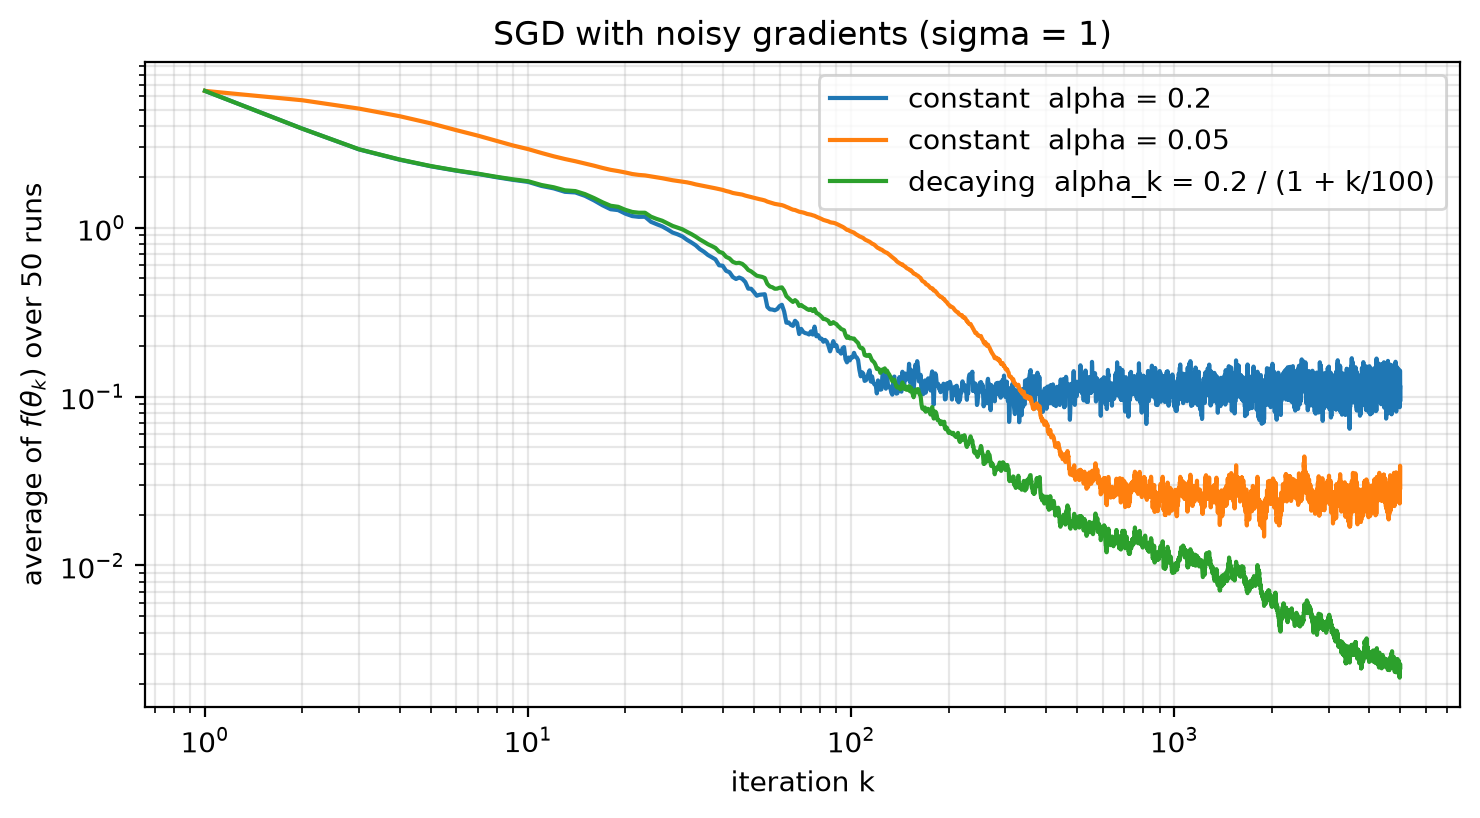
\includegraphics[width=0.78\textwidth]{figures/sgd_noise.png}

\small 잡음이 있는 gradient로 SGD를 했을 때 $f(\theta_k)$의 평균 ($50$번 반복, 로그-로그 눈금)
\end{center}
}{%
\begin{center}
\fbox{\parbox{0.8\textwidth}{\centering\small
[그림 자리] \texttt{figures/sgd\_noise.png}\\
\texttt{sgd\_noise\_2d.py}를 실행하면 생성된다.}}
\end{center}
}

\begin{center}
\begin{tabular}{@{}lcc@{}}
\toprule
학습률 & 이론값 $\lim\mathbb E[f]$ & 실험값 (마지막 $500$단계 평균) \\
\midrule
$\alpha=0.2$ (일정) & $0.113$ & $0.114$ \\
$\alpha=0.05$ (일정) & $0.026$ & $0.027$ \\
$\alpha_k=0.2/(1+k/100)$ (감소) & $0$으로 감소 & $0.0026$ (계속 감소 중) \\
\bottomrule
\end{tabular}
\end{center}

\paragraph{6. 학습률을 줄여 가면: Robbins--Monro 조건.}
잡음의 바닥을 없애려면 학습률을 점점 줄여야 한다. 얼마나 빨리 줄여야 할까?
Robbins와 Monro(1951)의 조건은
\[
\boxed{
\sum_{k=0}^{\infty}\alpha_k=\infty,
\qquad
\sum_{k=0}^{\infty}\alpha_k^2<\infty
}
\]
이다.
\begin{itemize}[leftmargin=1.8em]
\item $\sum\alpha_k=\infty$: 갈 수 있는 \textbf{총 거리}가 무한해야 한다.
학습률을 너무 빨리 줄이면 (예: $\alpha_k=\frac{1}{(k+1)^2}$, 합이 유한) 최솟값에 닿기 전에 멈춰 버릴 수 있다.
\item $\sum\alpha_k^2<\infty$: 3에서 잡음이 매 단계 더하는 양은 $\frac{M\alpha_k^2\sigma^2}{2}$이므로,
그 \textbf{총합이 유한}해야 잡음이 계속 쌓이지 않는다. 학습률이 일정하면 이 합이 무한이다.
\end{itemize}

\begin{center}
\begin{tabular}{@{}lccl@{}}
\toprule
학습률 $\alpha_k$ & $\sum\alpha_k$ & $\sum\alpha_k^2$ & 판정 \\
\midrule
$\alpha$ (일정) & $\infty$ & $\infty$ & 바닥에서 멈춤 \\
$\alpha_0/(1+k/k_0)$ ($\propto\frac1k$) & $\infty$ & 유한 & 조건 만족 \\
$\alpha_0/\sqrt{k+1}$ & $\infty$ & $\infty$ & 경계 (둘째 조건 불만족) \\
$\alpha_0/(k+1)^2$ & 유한 & 유한 & 너무 빨리 줄어듦 \\
\bottomrule
\end{tabular}
\end{center}

이 조건 아래에서 대표적으로 다음이 알려져 있다 (증명은 생략한다).
\begin{itemize}[leftmargin=1.8em]
\item 손실이 볼록(convex)하면 SGD는 최솟값으로 수렴한다.
\item 손실이 볼록하지 않으면 (신경망) gradient의 크기가 $0$으로 가는 점, 즉 \textbf{정류점(stationary point)}으로 수렴한다.
정류점은 극소점일 수도 있지만 안장점일 수도 있다.
\item 강볼록(strongly convex, 가장 작은 곡률이 $\mu>0$)인 경우 $\alpha_k\propto\frac1k$로 잡으면
$\mathbb E[L(\theta_k)]-L^*=O\!\left(\frac1k\right)$이다.
그림의 초록색 곡선이 로그-로그 눈금에서 기울기 약 $-1$인 직선처럼 내려가는 것이 이것이다.
잡음이 없는 경사하강법은 $(1-\alpha\mu)^k$처럼 \textbf{지수적으로} 빨리 줄어드는 것과 비교된다.
\end{itemize}

\paragraph{7. 실무와의 연결.}
\begin{itemize}[leftmargin=1.8em]
\item 실제 학습은 단계 수가 정해져 있으므로 Robbins--Monro 조건을 문자 그대로 따르지는 않지만,
\textbf{학습률 스케줄}(\ref{app:opt}.1절의 cosine 감소, 일정 epoch마다 $\frac1{10}$로 줄이는 step decay 등)은
모두 ``처음에는 크게 움직이고, 나중에는 잡음의 바닥을 낮추기 위해 학습률을 줄인다''는 같은 생각에서 나왔다.
\item 미니배치 크기 $h$를 키우면 $\sigma^2\propto\frac1h$가 작아져 바닥이 낮아진다.
학습률을 줄이는 것과 배치를 키우는 것이 비슷한 효과를 내는 이유이다.
\item 본문의 RMSProp 그림에서 최솟값 근처의 흔들림, \ref{sec:mnistopt}절의 MNIST 손실이 들쭉날쭉한 것도
같은 원리로 이해할 수 있다.
\item Adam 같은 적응적 방법도 이론적인 수렴 보장에는 주의가 필요하다.
볼록한 문제에서도 원래의 Adam이 수렴하지 않는 예가 알려져 있으며 (Reddi 등, 2018),
이를 고친 변형(AMSGrad 등)이 제안되었다. 실무에서는 대개 학습률 스케줄과 함께 사용한다.
\end{itemize}

% -------------------------------------------------
\subsection{Newton 방법을 그대로 쓸 수 없는 이유}
% -------------------------------------------------

``Gradient Descent와 Newton's method'' 시간에 본 Newton 방법은
\[
\theta_{k+1}=\theta_k-H_k^{-1}g_k
\]
였다. $H_k^{-1}$이 곡률이 큰 방향의 보폭은 줄이고 작은 방향의 보폭은 키워 주므로,
2차 함수에서는 \textbf{한 번에} 최솟값에 도달한다.
본문의 예제 $f(x,y)=\frac{1}{20}x^2+y^2$에서는 $H=\operatorname{diag}\bigl(\frac{1}{10},\,2\bigr)$이므로
\[
\theta_1=\begin{pmatrix}-7\\2\end{pmatrix}-\begin{pmatrix}10&0\\0&\tfrac12\end{pmatrix}\begin{pmatrix}-0.7\\4\end{pmatrix}
=\begin{pmatrix}0\\0\end{pmatrix}
\]
로 바로 최솟값이다. 그런데 신경망에서는 이것을 쓸 수 없다.

매개변수가 $n$개이면 $H$는 $n\times n$ 행렬이다.
\begin{itemize}[leftmargin=1.8em]
\item 지난주 MNIST의 작은 network만 해도 $n\approx8\times10^4$이므로 $H$의 원소는 약 $6.3\times10^9$개,
실수 하나에 8바이트이면 약 $50$GB이다.
\item 역행렬(또는 연립방정식 $Hp=-g$의 풀이)에는 $O(n^3)$의 계산이 든다.
\item 언어모델은 $n$이 수십억 이상이므로 아예 불가능하다.
\end{itemize}

\begin{center}
\begin{tabular}{@{}lll@{}}
\toprule
방법 & 메모리 & 한 단계의 계산량 \\
\midrule
SGD & $O(n)$ & $O(n)$ \\
모멘텀, Adam & $O(n)$ (상태 $1\sim2$개) & $O(n)$ \\
Newton & $O(n^2)$ & $O(n^3)$ \\
BFGS & $O(n^2)$ & $O(n^2)$ \\
L-BFGS & $O(mn)$ & $O(mn)$ \\
\bottomrule
\end{tabular}
\end{center}
(gradient 자체를 구하는 역전파의 비용은 모든 방법에 공통이므로 제외하였다. $m$은 L-BFGS가 기억하는 쌍의 개수.)

% -------------------------------------------------
\subsection{Quasi-Newton 방법: BFGS}
% -------------------------------------------------

\paragraph{아이디어: gradient의 변화로 곡률을 추정한다.}
Hessian을 직접 계산하지 않고, \textbf{이미 계산한 gradient들의 변화}로부터 곡률을 추정할 수 있다.
1변수라면
\[
f''(x_k)\approx\frac{f'(x_{k+1})-f'(x_k)}{x_{k+1}-x_k}
\]
인 것과 같은 생각이다.
연속한 두 단계에서
\[
s_k=\theta_{k+1}-\theta_k,
\qquad
y_k=g_{k+1}-g_k
\]
라 하면, 2차 함수 $L(\theta)=\frac12\theta\T A\theta$에서는 $g=A\theta$이므로 정확히 $y_k=As_k$이다.
일반적인 함수에서도 근사적으로
\[
\boxed{
H_{k+1}s_k\approx y_k
}
\qquad\text{(secant 조건)}
\]
가 성립한다.

\paragraph{BFGS의 갱신식.}
BFGS(Broyden--Fletcher--Goldfarb--Shanno)는 Hessian의 역행렬의 근사 $B_k\approx H_k^{-1}$을 직접 갱신한다.
새 근사 $B_{k+1}$이 secant 조건 $B_{k+1}y_k=s_k$를 만족하면서 $B_k$와 가장 가깝도록 정하면
\[
\boxed{
B_{k+1}=\bigl(I-\rho_k s_ky_k\T\bigr)\,B_k\,\bigl(I-\rho_k y_ks_k\T\bigr)+\rho_k s_ks_k\T,
\qquad
\rho_k=\frac{1}{y_k\T s_k}
}
\]
를 얻는다. 그리고 Newton 방향 대신
\[
p_k=-B_kg_k,
\qquad
\theta_{k+1}=\theta_k+t_k\,p_k
\]
로 움직인다. 이동 거리 $t_k$는 \textbf{line search}로 정한다.
\begin{itemize}[leftmargin=1.8em]
\item $y_k\T s_k>0$ (\textbf{곡률 조건})이면 $B_k$가 양의 정부호이면 $B_{k+1}$도 양의 정부호로 유지되어,
$p_k$가 항상 함수값이 줄어드는 방향($g_k\T p_k<0$)이 된다.
\item 2차 함수에서 정확한 line search를 쓰면 BFGS는 최대 $n$번 만에 최솟값에 도달한다.
\end{itemize}

\paragraph{Line search란?}
지금까지의 방법들은 학습률 $\alpha$라는 \textbf{정해진 보폭}으로 움직였다.
line search는 보폭을 미리 정하지 않는다.
먼저 갈 방향 $p_k$를 정한 뒤, 그 방향의 직선 $\theta_k+t\,p_k$ 위에서
\textbf{얼마나 갈지} $t$를 몇 번 시험해 보며 고른다.
예를 들어 $t=1$을 먼저 해 보고, 함수값이 충분히 줄지 않으면 $t$를 줄여서 다시 해 보는 식이다.
이때 확인하는 것은 두 가지이다.
\begin{itemize}[leftmargin=1.8em]
\item \textbf{너무 멀리 가지 않았는가}: 함수값이 충분히 줄었는가 (Armijo 조건)
\item \textbf{너무 덜 가지 않았는가}: 그 방향으로 아직 가파르게 내려가는 중은 아닌가 (곡률 조건)
\end{itemize}
좋은 보폭을 자동으로 찾아 주는 대신,
$t$를 하나 시험할 때마다 \textbf{함수값과 gradient를 다시 계산}해야 한다는 비용이 든다.

\paragraph{Line search: Wolfe 조건.}
수식으로는 $t_k$를 보통 다음 두 조건을 만족하는 값으로 정한다 ($0<c_1<c_2<1$, 예: $c_1=10^{-4}$, $c_2=0.9$).
\[
\begin{aligned}
&L(\theta_k+t\,p_k)\le L(\theta_k)+c_1\,t\,g_k\T p_k
&&\text{(충분히 감소: Armijo 조건)}\\
&\bigl|\nabla L(\theta_k+t\,p_k)\T p_k\bigr|\le c_2\,\bigl|g_k\T p_k\bigr|
&&\text{(기울기가 충분히 완만해짐: strong Wolfe 조건)}
\end{aligned}
\]
두 번째 조건이 곡률 조건 $y_k\T s_k>0$을 보장한다.
line search는 조건을 만족하는 $t$를 찾을 때까지 \textbf{함수값과 gradient를 여러 번 계산}한다는 점에 주목하자.

BFGS도 $B_k$라는 $n\times n$ 행렬을 저장해야 하므로 신경망에는 여전히 너무 크다.

% -------------------------------------------------
\subsection{L-BFGS: 최근 $m$개의 쌍만 기억한다}
% -------------------------------------------------

\textbf{L-BFGS}(Limited-memory BFGS)는 $B_k$를 저장하지 않는다.
대신 최근 $m$개(보통 $5\sim20$개)의 쌍 $(s_i,y_i)$만 기억하고,
BFGS 갱신식을 $m$번 적용했을 때의 $B_kg_k$를 다음 \textbf{two-loop recursion}으로 바로 계산한다.

\begin{remarkbox}[L-BFGS의 two-loop recursion: $r\approx B_kg_k$ 계산]
\begin{enumerate}[leftmargin=1.8em]
\item $q\leftarrow g_k$
\item $i=k-1,\ k-2,\ \ldots,\ k-m$에 대하여:\quad
$a_i\leftarrow\rho_i\,s_i\T q,\qquad q\leftarrow q-a_i\,y_i$
\item $r\leftarrow\gamma_k\,q$,\quad $\gamma_k=\dfrac{s_{k-1}\T y_{k-1}}{y_{k-1}\T y_{k-1}}$
\quad (처음 근사 $B_k^{(0)}=\gamma_kI$)
\item $i=k-m,\ \ldots,\ k-1$에 대하여:\quad
$b\leftarrow\rho_i\,y_i\T r,\qquad r\leftarrow r+s_i\,(a_i-b)$
\item 방향 $p_k=-r$
\end{enumerate}
벡터의 내적과 덧셈만 쓰므로 메모리와 계산량이 모두 $O(mn)$이다.
\end{remarkbox}

\paragraph{예제 함수에서의 L-BFGS.}
본문의 예제는 2차 함수이므로 Hessian이 상수이고, 앞에서 보았듯이 Newton 방법이면 \textbf{한 번}에 끝난다.
그런데도 L-BFGS를 적용해 보는 것은, 실제 신경망에서는 Newton 방법을 쓸 수 없고
실무에서 쓸 수 있는 2차 방법이 Hessian을 gradient의 변화로 근사하는 quasi-Newton 방법,
특히 L-BFGS이기 때문이다.
\textbf{Hessian을 한 번도 계산하지 않고도} 1차 방법보다 훨씬 빨리 수렴하는 모습을 확인해 보자.
PyTorch에는 \texttt{torch.optim.LBFGS}로 구현되어 있다.
L-BFGS는 line search 도중 함수값을 여러 번 다시 계산해야 하므로,
\textbf{손실을 다시 계산하는 함수(\texttt{closure})}를 \texttt{step}에 넘겨 준다.
이것이 다른 optimizer와 다른 점이다.

\begin{lstlisting}
import torch

w = torch.tensor([-7.0, 2.0], requires_grad=True)       # (x, y), start point

def f(w):
    return w[0] ** 2 / 20.0 + w[1] ** 2

# max_iter=1: one L-BFGS iteration per optimizer.step() (the default is 20)
optimizer = torch.optim.LBFGS([w], lr=1.0, max_iter=1, history_size=10,
                              line_search_fn="strong_wolfe")

n_eval = 0
def closure():                  # L-BFGS may evaluate f several times per step
    global n_eval
    n_eval += 1
    optimizer.zero_grad()
    loss = f(w)
    loss.backward()
    return loss

for k in range(1, 9):
    optimizer.step(closure)
    print(f"iteration {k}: (x, y) = ({w[0].item():9.6f}, {w[1].item():9.6f}),  "
          f"f = {f(w).item():.3e},  evaluations so far = {n_eval}")
\end{lstlisting}

\begin{center}
\begin{minipage}[c]{0.5\textwidth}
\centering
\begin{tabular}{@{}crrc@{}}
\toprule
반복 & \multicolumn{1}{c}{$x$} & \multicolumn{1}{c}{$y$} & $f$ \\
\midrule
1 & $-6.8511$ & $1.1489$ & $3.7\times10^{0}$ \\
2 & $-6.2977$ & $-0.0551$ & $2.0\times10^{0}$ \\
3 & $-5.9080$ & $-0.1358$ & $1.8\times10^{0}$ \\
4 & $-1.5216$ & $-0.3675$ & $2.5\times10^{-1}$ \\
5 & $-0.0928$ & $-0.0878$ & $8.1\times10^{-3}$ \\
6 & $0.0197$ & $-0.0050$ & $4.5\times10^{-5}$ \\
7 & $0.0024$ & $-0.0002$ & $3.1\times10^{-7}$ \\
8 & $0.0000$ & $0.0000$ & $9.3\times10^{-11}$ \\
\bottomrule
\end{tabular}
\end{minipage}%
\begin{minipage}[c]{0.48\textwidth}
\centering
\IfFileExists{figures/opt_lbfgs.png}{%
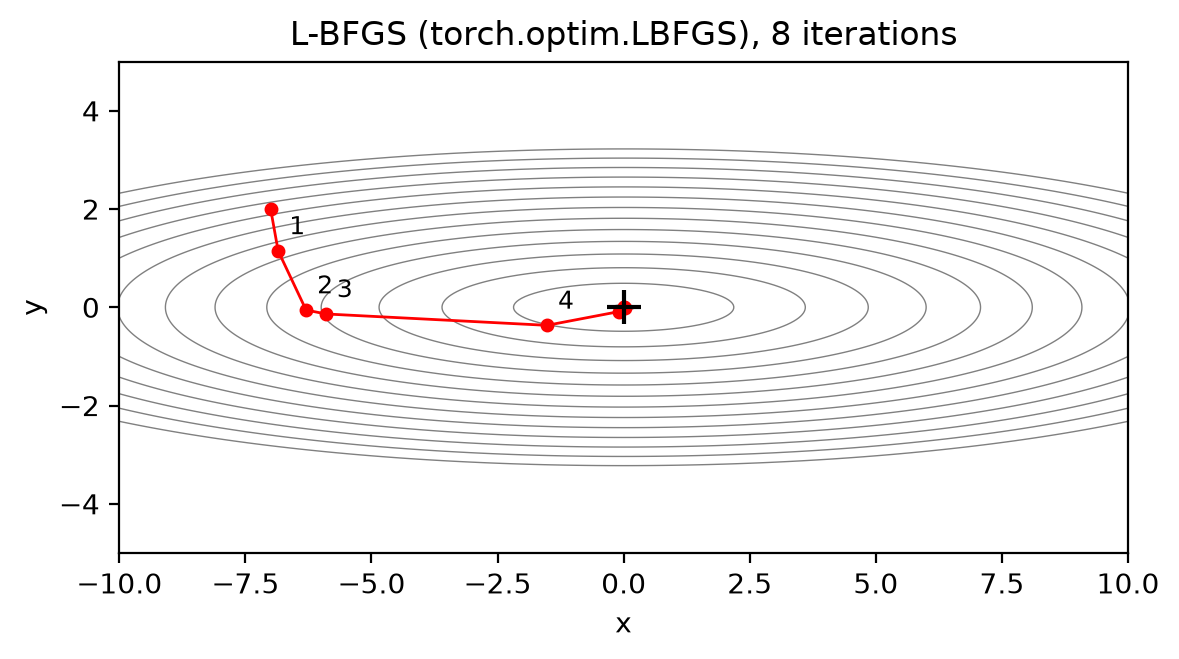
\includegraphics[width=\textwidth]{figures/opt_lbfgs.png}
}{%
\fbox{\parbox{0.9\textwidth}{\centering\small
[그림 자리] \texttt{figures/opt\_lbfgs.png}}}
}
\end{minipage}
\end{center}

\begin{itemize}[leftmargin=1.8em]
\item 첫 반복에서는 아직 쌍 $(s,y)$가 없으므로 gradient 방향으로 움직인다.
쌍이 쌓이면서 곡률을 반영한 방향으로 바뀌고, 4번째 반복부터 최솟값을 향해 크게 이동한다.
\item $8$번의 반복(함수값 계산 $16$번)만에 $f\approx10^{-10}$에 도달하였다.
본문에서 $30$번 갱신한 SGD, 모멘텀, AdaGrad, Adam은 $f\approx10^{-1}\sim10^{-3}$이었다.
\item 이론적으로 2차 함수에서는 $n=2$번 만에 끝나야 하지만,
PyTorch의 line search는 Wolfe 조건만 만족하면 멈추는 근사적인 방법이라 조금 더 걸린다.
\end{itemize}

% -------------------------------------------------
\subsection{L-BFGS가 딥러닝에서 잘 쓰이지 않는 이유}
% -------------------------------------------------

예제에서는 훨씬 빨랐는데, 왜 신경망 학습에는 Adam이나 SGD를 쓸까?

\paragraph{1. 미니배치 잡음.}
L-BFGS는 정확한 gradient를 가정한다.
그런데 미니배치 학습에서는 단계마다 다른 데이터 $\mathcal B_k$로 gradient를 계산한다.
미니배치 gradient를 $\nabla L_{\mathcal B}(\theta)=\nabla L(\theta)+\xi_{\mathcal B}$ (잡음 $\xi$)로 쓰면
\[
y_k=\nabla L_{\mathcal B_{k+1}}(\theta_{k+1})-\nabla L_{\mathcal B_k}(\theta_k)
=\underbrace{\nabla L(\theta_{k+1})-\nabla L(\theta_k)}_{\approx H s_k}
+\underbrace{\xi_{\mathcal B_{k+1}}-\xi_{\mathcal B_k}}_{\text{잡음}}
\]
이다. 보폭 $s_k$가 작아지면 첫 항은 $s_k$에 비례해 작아지지만 잡음 항은 줄지 않는다.
그래서 $y_k$와 $s_k$로 추정한 곡률이 \textbf{곡률이 아니라 데이터의 차이}를 반영하게 되어 근사가 무너진다
(곡률 조건 $y_k\T s_k>0$도 깨질 수 있다).
두 gradient를 같은 미니배치로 계산하는 변형들이 연구되었지만 널리 쓰이지는 않는다.

\paragraph{2. Line search의 비용.}
한 단계마다 함수값과 gradient를 여러 번 계산해야 한다.
큰 network에서 순전파와 역전파 한 번은 비싸므로,
그 계산으로 SGD나 Adam을 여러 걸음 가는 편이 대개 더 효율적이다.
게다가 미니배치 손실로 하는 line search 자체도 잡음 때문에 불안정하다.

\paragraph{3. 비볼록성.}
신경망의 손실함수는 볼록하지 않아 Hessian이 양의 정부호가 아닐 수 있다.
안장점(saddle point) 근처에서는 Hessian의 고유값이 음수인 방향이 있어서,
Newton 방향 $-H^{-1}g$가 오히려 함수값이 \textbf{올라가는} 방향일 수 있다.
quasi-Newton 방법은 곡률 조건을 만족하는 쌍만 쓰는 등의 장치로 이를 피하지만, 그만큼 곡률 정보가 부정확해진다.

\paragraph{4. 메모리.}
$m$개의 쌍만 저장해도 매개변수 전체를 $2m$번 복사해 두는 것과 같다.
$m=10$이면 매개변수의 $20$배이므로, 큰 모델에서는 상태를 $2$개만 가지는 Adam보다 훨씬 무겁다.

% -------------------------------------------------
\subsection{L-BFGS가 실제로 쓰이는 곳}
% -------------------------------------------------

반대로 위의 약점이 문제가 되지 않는 곳, 즉
\textbf{데이터 전체로 정확한 gradient를 계산할 수 있고, 높은 정밀도가 중요한} 문제에서는 L-BFGS가 매우 강력하다.

\begin{itemize}[leftmargin=1.8em]
\item \textbf{작은 문제의 full-batch 학습.}
scikit-learn의 로지스틱 회귀(\texttt{LogisticRegression})는 기본 solver가 \texttt{"lbfgs"}이다.
\item \textbf{PINN (Physics-Informed Neural Network).}
신경망 $u_\theta(x,t)$로 편미분방정식의 해를 근사하는 과학계산 방법이다.
예를 들어 방정식 $\mathcal N[u]=0$과 경계조건 $u=h$가 주어지면
\[
L(\theta)=\frac{1}{N_r}\sum_{i=1}^{N_r}\bigl|\mathcal N[u_\theta](x_i)\bigr|^2
+\frac{1}{N_b}\sum_{j=1}^{N_b}\bigl|u_\theta(x_j)-h(x_j)\bigr|^2
\]
을 최소화한다 (첫 항: 방정식의 잔차, 둘째 항: 경계조건).
점 $x_i$, $x_j$를 전체 배치로 쓸 수 있고 해의 정밀도가 중요하므로,
\textbf{Adam으로 먼저 대략 학습한 뒤 L-BFGS로 마무리}하는 방식이 표준처럼 쓰인다.
\item \textbf{신경 스타일 전이 (neural style transfer).}
network의 가중치가 아니라 \textbf{이미지 한 장}을 최적화하는 문제라 full-batch이므로 L-BFGS를 썼다 (Gatys 등).
\end{itemize}

\begin{thinkbox}[데이터 계산 과학과 L-BFGS]
수치해석과 과학계산에서는 L-BFGS가 오래전부터 표준적인 최적화 방법이었다.
딥러닝이 과학계산 문제(PINN, 역문제, 대리 모델 등)에 쓰이면서,
``미니배치 + Adam''과 ``full-batch + L-BFGS''를 상황에 맞게 함께 쓰는 일이 많아졌다.
어떤 경우에 어느 쪽이 유리한지는 위의 네 가지 이유로 판단할 수 있다.
\end{thinkbox}

% -------------------------------------------------
\subsection{대규모 딥러닝에서의 ``곡률 근사''}\label{app:largescale}
% -------------------------------------------------

Hessian을 통째로 다룰 수는 없지만, 곡률 정보를 \textbf{구조를 단순화하여} 근사하는 방법들이 있다.
모두 다음과 같은 \textbf{preconditioning}의 형태로 볼 수 있다.
\[
\boxed{
\theta_{k+1}=\theta_k-\alpha\,P_k^{-1}g_k
}
\]
\begin{center}
\begin{tabular}{@{}ll@{}}
\toprule
방법 & preconditioner $P_k$ \\
\midrule
SGD & $I$ \\
Newton & $H_k$ (전체 Hessian) \\
AdaGrad, RMSProp, Adam & $\operatorname{diag}(\sqrt{h_k})$ 또는 $\operatorname{diag}(\sqrt{\hat v_k})$ (대각 행렬) \\
K-FAC, Shampoo & 층마다 (작은 행렬) $\otimes$ (작은 행렬) 꼴 \\
\bottomrule
\end{tabular}
\end{center}

\paragraph{Adam은 대각 근사이다.}
Adam이 $\sqrt{\hat v}$로 나누는 것은 매개변수마다(대각 성분마다) 보폭을 조절하는 것이다.
$\hat v$는 Hessian 자체는 아니지만 gradient 제곱의 평균으로 곡률의 크기를 대신하는 역할을 하며,
본문에서 ``AdaGrad가 Newton의 곡률 보정과 비슷한 효과''라고 한 것이 이 뜻이다.
그러나 대각 행렬은 매개변수 \textbf{사이의} 관계(Hessian의 비대각 성분)를 반영하지 못한다.

\paragraph{Hessian-free 방법.}
Newton 방향은 연립방정식 $H_kp=-g_k$의 해이다.
$H_k$를 만들지 않고도 \textbf{Hessian과 벡터의 곱} $H_kv$는
\[
H_kv=\nabla_\theta\bigl(\nabla_\theta L(\theta)\T v\bigr)
\]
로, 역전파를 한 번 더 하는 정도의 비용으로 계산할 수 있다.
켤레기울기법(conjugate gradient)은 행렬 대신 이 곱만 사용하여 $H_kp=-g_k$를 근사적으로 푸므로,
$H_k$를 저장하지 않고 Newton 방향을 근사할 수 있다 (Martens, 2010).

\paragraph{K-FAC.}
한 affine 계층 $A=XW$ ($X$: $h\times l$, $W$: $l\times m$)에서
지난주에 $\pd{L}{W}=X\T\delta$ ($\delta=\pd{L}{A}$, $h\times m$)를 얻었다.
K-FAC은 이 층의 곡률 행렬(정확히는 Fisher 정보 행렬)을 입력 쪽 통계
$\bar A=\frac1h X\T X$ ($l\times l$)와 출력 쪽 통계 $\bar G=\frac1h\delta\T\delta$ ($m\times m$)의
\textbf{크로네커 곱}으로 근사한다. 그러면 $(lm)\times(lm)$ 행렬 대신 작은 두 행렬의 역행렬만 있으면 되고,
갱신 방향은
\[
\Delta W=-\alpha\,\bar A^{-1}\,\pd{L}{W}\,\bar G^{-1}
\]
꼴이 된다 (실제로는 역행렬이 잘 정의되도록 작은 값을 더한다).

\paragraph{Shampoo.}
층의 gradient 행렬 $G_k=\pd{L}{W}$ ($l\times m$)에 대해 양쪽 통계를 누적하여
\[
L_k=\sum_{j\le k}G_jG_j\T\ (l\times l),
\qquad
R_k=\sum_{j\le k}G_j\T G_j\ (m\times m),
\qquad
W_{k+1}=W_k-\alpha\,L_k^{-1/4}\,G_k\,R_k^{-1/4}
\]
로 갱신한다. 매개변수가 하나뿐이면 $L_k=R_k=\sum g_j^2$이므로 $G_k/\sqrt{\sum g_j^2}$,
즉 AdaGrad와 같아진다. Shampoo는 \textbf{AdaGrad를 행렬로 확장}한 방법이다.

\paragraph{Muon.}
층의 gradient로 모멘텀 $M_k=\beta M_{k-1}+G_k$를 만든 뒤,
$M_k$의 특이값 분해 $M_k=U\Sigma V\T$에서 특이값을 모두 $1$로 바꾼 행렬 $UV\T$
(가장 가까운 직교 행렬)의 방향으로 갱신한다.
\[
W_{k+1}=W_k-\alpha\,\operatorname{orth}(M_k),
\qquad
\operatorname{orth}(M)=UV\T
\]
특이값 분해는 비싸므로 실제로는 행렬곱만 쓰는 Newton--Schulz 반복으로 $UV\T$를 근사한다.
모든 방향의 크기를 고르게 맞춘다는 점에서 역시 곡률 보정의 한 형태로 볼 수 있다.
Shampoo와 Muon은 최근 대규모 모델 학습에서 실제로 쓰이기 시작했지만,
아직 AdamW만큼 표준은 아니다.

\begin{keybox}[부록 정리]
\begin{itemize}[leftmargin=1.5em]
\item 요즘 실무의 기본은 \textbf{AdamW}, 이미지 분류 CNN에서는 \textbf{SGD + 모멘텀}이다.
AdaGrad는 RMSProp, Adam으로 이어지는 아이디어의 출발점으로 배운다.
\item optimizer만큼, 때로는 그보다 \textbf{학습률 스케줄}과 weight decay가 중요하다.
\item 잡음이 있는 gradient로 학습률을 고정하면 SGD는 $\alpha\sigma^2$에 비례하는 \textbf{잡음의 바닥}에서 멈춘다.
$\sum\alpha_k=\infty$, $\sum\alpha_k^2<\infty$ (Robbins--Monro)를 만족하도록 학습률을 줄이면 수렴한다.
\item Newton 방법은 $O(n^2)$ 메모리, $O(n^3)$ 계산 때문에 신경망에 쓸 수 없다.
\item L-BFGS는 gradient의 변화로 곡률을 근사하여 $O(mn)$로 줄인다.
full-batch로 정밀하게 풀어야 하는 문제(PINN, 작은 모델)에서는 강력하지만,
미니배치 잡음, line search 비용, 비볼록성, 메모리 때문에 대규모 딥러닝에서는 잘 쓰이지 않는다.
\item 대규모 딥러닝의 곡률 활용은 \textbf{구조를 단순화한 preconditioner}로 이루어진다:
Adam(대각), K-FAC과 Shampoo(층별 크로네커 곱), Muon(직교화).
\end{itemize}
\end{keybox}


\end{document}
